% -*- program: xelatex -*-

\documentclass[10pt
	]{beamer}

% -----------------------------------------------------------------------------
% theming
\usetheme[numbering=fraction,
	progressbar=frametitle,
	% background=dark
	]{metropolis}


% % use a heavier font for large room/underpowered projector
% \setsansfont[BoldFont={Fira Sans SemiBold}]{Fira Sans Book}

% % can use every beamer color theme!
% \usecolortheme{crane}
% \useoutertheme{metropolis}
% \useinnertheme{metropolis}
% \usefonttheme{metropolis}

% % or set colors by hand
\definecolor{myblue}{rgb}{0.047, 0.298, 0.435}
\definecolor{myalert}{rgb}{0.847, 0.510, 0.106}

% change header color
\setbeamercolor{frametitle}{bg=myblue}
% \setbeamercolor{...}{fg=...,bg=...}
% \setbeamercolor{progress bar}{...}
% \setbeamercolor{title separator}{...}
% \setbeamercolor{progress bar in head/foot}{...}
% \setbeamercolor{progress bar in section page}{...}

% slightly darker organce
\setbeamercolor{alerted text}{fg=myalert}



% change width of title separator, section page separator % progress
%https://github.com/matze/mtheme/issues/237
\makeatletter
\setlength{\metropolis@titleseparator@linewidth}{1pt}
\setlength{\metropolis@progressonsectionpage@linewidth}{1.5pt}
\setlength{\metropolis@progressinheadfoot@linewidth}{1.5pt}
\makeatother


% environment for alerts (=colored bullet)
% http://tex.stackexchange.com/questions/14319/beamer-change-individual-bullet-color-in-itemize-list
\newenvironment{aleenv}{\only{\setbeamercolor{local structure}{fg=myalert}}}{}

% Put graphic anywhere on slide using Put(x, y){}
% with x, y in pt
% http://tex.stackexchange.com/questions/34921/how-to-overlap-images-in-a-beamer-slide
\def\Put(#1,#2)#3{\leavevmode\makebox(0,0){\put(#1,#2){#3}}}


% -----------------------------------------------------------------------------
% do not count appendix slides, use \appendix to indicate 
\usepackage{appendixnumberbeamer}  
% creative commons icons
\usepackage[scale=2
	]{ccicons} 
% fontawesome font/icons
\usepackage{fontspec}
\usepackage{fontawesome}      %
\usepackage{pifont}
% Graphics
\usepackage{graphicx}
\usepackage{tikz}
\usetikzlibrary{shapes, arrows, positioning, calc, arrows.meta, snakes}
\usepackage{adjustbox}

% use speaker notes
\usepackage{pgfpages}
\setbeameroption{hide notes} % Only slides
%\setbeameroption{show only notes} % Only notes
% \setbeameroption{show notes on second screen=right} % Both


% for overview.tikz figure
\newlength\yearposx


%%% ---------------------------------------------------------------------------
\title{Statistical Eco(-toxico)logy}
\subtitle{Improving the Utilisation of Data for\\Environmental Risk Assessment}
\date{25\textsuperscript{th} January 2017}
\author{Eduard Sz\"{o}cs}



%%% ---------------------------------------------------------------------------
\begin{document}

%%% ------------------------------
\maketitle

\begin{frame}{Table of contents}
  \setbeamertemplate{section in toc}[sections numbered]
  \tableofcontents[hideallsubsections]
\end{frame}


%%% ---------------------------------------------------------------------------
{%
\setbeamertemplate{frame footer}{WWF (2016), Living Planet Report; Vörösmarty (2010). Nature.
}
\begin{frame}[t]
\frametitle{Freshwater biodiversity is strongly declining}
	\begin{columns}[T]
	\column{.66\textwidth}
		\onslide<1->{
			\resizebox{\textwidth}{!}{%
						% Created by tikzDevice version 0.10.1 on 2017-01-20 09:42:50
% !TEX encoding = UTF-8 Unicode
\begin{tikzpicture}[x=1pt,y=1pt]
\definecolor{fillColor}{RGB}{255,255,255}
\path[use as bounding box,fill=fillColor,fill opacity=0.00] (0,0) rectangle (505.89,405.01);
\begin{scope}
\path[clip] (  0.00,  0.00) rectangle (505.89,405.01);
\definecolor{drawColor}{RGB}{255,255,255}
\definecolor{fillColor}{RGB}{255,255,255}

\path[draw=drawColor,line width= 0.6pt,line join=round,line cap=round,fill=fillColor] (  0.00,  0.00) rectangle (505.89,405.01);
\end{scope}
\begin{scope}
\path[clip] ( 58.39, 81.11) rectangle (498.89,376.10);
\definecolor{fillColor}{RGB}{255,255,255}

\path[fill=fillColor] ( 58.39, 81.11) rectangle (498.89,376.10);
\definecolor{drawColor}{RGB}{70,130,180}

\path[draw=drawColor,line width= 1.7pt,line join=round] ( 80.80,274.77) --
	( 86.76,266.71) --
	( 96.30,264.51) --
	(106.43,265.24) --
	(122.52,257.91) --
	(137.41,246.92) --
	(154.69,242.53) --
	(175.55,235.93) --
	(191.04,227.14) --
	(201.77,222.74) --
	(211.90,211.02) --
	(226.20,206.63) --
	(238.72,194.90) --
	(248.85,178.05) --
	(269.70,174.39) --
	(277.45,167.06) --
	(292.94,165.59) --
	(307.25,159.00) --
	(316.78,159.00) --
	(337.64,151.67) --
	(358.49,142.88) --
	(385.91,135.55) --
	(403.78,135.55) --
	(416.89,130.42) --
	(431.19,128.96) --
	(444.90,135.55) --
	(452.05,140.68) --
	(468.14,131.89) --
	(478.87,128.23);
\definecolor{drawColor}{RGB}{0,0,139}

\path[draw=drawColor,line width= 1.7pt,line join=round] ( 78.42,274.03) --
	( 95.08,263.81) --
	(109.95,266.73) --
	(126.61,269.65) --
	(144.46,266.00) --
	(153.98,260.90) --
	(164.09,260.17) --
	(179.56,251.41) --
	(196.82,245.57) --
	(208.72,239.00) --
	(221.81,229.52) --
	(235.49,220.03) --
	(249.77,211.28) --
	(272.97,214.19) --
	(301.53,210.55) --
	(330.69,207.63) --
	(357.46,207.63) --
	(389.00,208.36) --
	(419.93,209.09) --
	(430.64,212.74) --
	(449.09,209.09) --
	(467.53,210.55) --
	(477.65,210.55);
\definecolor{drawColor}{RGB}{0,139,0}

\path[draw=drawColor,line width= 1.7pt,line join=round] ( 80.83,275.43) --
	(103.50,267.98) --
	(130.37,265.85) --
	(153.89,250.95) --
	(162.28,248.83) --
	(172.36,253.08) --
	(183.28,252.02) --
	(210.15,245.63) --
	(246.26,245.63) --
	(279.85,240.31) --
	(324.36,228.61) --
	(344.51,230.73) --
	(362.14,220.09) --
	(373.90,221.16) --
	(383.98,217.96) --
	(412.53,217.96) --
	(421.77,224.35) --
	(441.08,212.64) --
	(452.00,215.84) --
	(478.87,206.26);
\definecolor{drawColor}{RGB}{0,0,0}

\path[draw=drawColor,line width= 0.6pt,dash pattern=on 1pt off 3pt ,line join=round] ( 58.39,273.30) -- (498.89,273.30);
\definecolor{drawColor}{gray}{0.50}

\path[draw=drawColor,line width= 0.6pt,line join=round,line cap=round] ( 58.39, 81.11) rectangle (498.89,376.10);
\end{scope}
\begin{scope}
\path[clip] (  0.00,  0.00) rectangle (505.89,405.01);
\definecolor{drawColor}{gray}{0.30}

\node[text=drawColor,anchor=base east,inner sep=0pt, outer sep=0pt, scale=  1.54] at ( 52.09, 83.90) {\bfseries 0.0};

\node[text=drawColor,anchor=base east,inner sep=0pt, outer sep=0pt, scale=  1.54] at ( 52.09,173.28) {\bfseries 0.5};

\node[text=drawColor,anchor=base east,inner sep=0pt, outer sep=0pt, scale=  1.54] at ( 52.09,262.67) {\bfseries 1.0};

\node[text=drawColor,anchor=base east,inner sep=0pt, outer sep=0pt, scale=  1.54] at ( 52.09,352.06) {\bfseries 1.5};
\end{scope}
\begin{scope}
\path[clip] (  0.00,  0.00) rectangle (505.89,405.01);
\definecolor{drawColor}{RGB}{0,0,0}

\path[draw=drawColor,line width= 0.6pt,line join=round] ( 54.89, 94.52) --
	( 58.39, 94.52);

\path[draw=drawColor,line width= 0.6pt,line join=round] ( 54.89,183.91) --
	( 58.39,183.91);

\path[draw=drawColor,line width= 0.6pt,line join=round] ( 54.89,273.30) --
	( 58.39,273.30);

\path[draw=drawColor,line width= 0.6pt,line join=round] ( 54.89,362.69) --
	( 58.39,362.69);
\end{scope}
\begin{scope}
\path[clip] (  0.00,  0.00) rectangle (505.89,405.01);
\definecolor{drawColor}{RGB}{0,0,0}

\path[draw=drawColor,line width= 0.6pt,line join=round] ( 76.63, 77.61) --
	( 76.63, 81.11);

\path[draw=drawColor,line width= 0.6pt,line join=round] (172.57, 77.61) --
	(172.57, 81.11);

\path[draw=drawColor,line width= 0.6pt,line join=round] (268.51, 77.61) --
	(268.51, 81.11);

\path[draw=drawColor,line width= 0.6pt,line join=round] (364.45, 77.61) --
	(364.45, 81.11);

\path[draw=drawColor,line width= 0.6pt,line join=round] (460.39, 77.61) --
	(460.39, 81.11);
\end{scope}
\begin{scope}
\path[clip] (  0.00,  0.00) rectangle (505.89,405.01);
\definecolor{drawColor}{gray}{0.30}

\node[text=drawColor,anchor=base,inner sep=0pt, outer sep=0pt, scale=  1.54] at ( 76.63, 64.19) {\bfseries 1970};

\node[text=drawColor,anchor=base,inner sep=0pt, outer sep=0pt, scale=  1.54] at (172.57, 64.19) {\bfseries 1980};

\node[text=drawColor,anchor=base,inner sep=0pt, outer sep=0pt, scale=  1.54] at (268.51, 64.19) {\bfseries 1990};

\node[text=drawColor,anchor=base,inner sep=0pt, outer sep=0pt, scale=  1.54] at (364.45, 64.19) {\bfseries 2000};

\node[text=drawColor,anchor=base,inner sep=0pt, outer sep=0pt, scale=  1.54] at (460.39, 64.19) {\bfseries 2010};
\end{scope}
\begin{scope}
\path[clip] (  0.00,  0.00) rectangle (505.89,405.01);
\definecolor{drawColor}{RGB}{0,0,0}

\node[text=drawColor,anchor=base,inner sep=0pt, outer sep=0pt, scale=  1.68] at (278.64, 47.02) {Year};
\end{scope}
\begin{scope}
\path[clip] (  0.00,  0.00) rectangle (505.89,405.01);
\definecolor{drawColor}{RGB}{0,0,0}

\node[text=drawColor,rotate= 90.00,anchor=base,inner sep=0pt, outer sep=0pt, scale=  1.68] at ( 22.62,228.61) {Index value (1970 = 1)};
\end{scope}
\begin{scope}
\path[clip] (  0.00,  0.00) rectangle (505.89,405.01);
\definecolor{fillColor}{RGB}{255,255,255}

\path[fill=fillColor] (157.35,  7.00) rectangle (399.93, 32.84);
\end{scope}
\begin{scope}
\path[clip] (  0.00,  0.00) rectangle (505.89,405.01);
\definecolor{drawColor}{RGB}{0,0,0}

\node[text=drawColor,anchor=base west,inner sep=0pt, outer sep=0pt, scale=  1.40] at (163.04, 15.10) {Habitat};
\end{scope}
\begin{scope}
\path[clip] (  0.00,  0.00) rectangle (505.89,405.01);
\definecolor{drawColor}{RGB}{0,139,0}

\path[draw=drawColor,line width= 4.6pt,line join=round] (215.15, 19.92) -- (226.71, 19.92);
\end{scope}
\begin{scope}
\path[clip] (  0.00,  0.00) rectangle (505.89,405.01);
\definecolor{drawColor}{RGB}{0,0,139}

\path[draw=drawColor,line width= 4.6pt,line join=round] (277.53, 19.92) -- (289.10, 19.92);
\end{scope}
\begin{scope}
\path[clip] (  0.00,  0.00) rectangle (505.89,405.01);
\definecolor{drawColor}{RGB}{70,130,180}

\path[draw=drawColor,line width= 4.6pt,line join=round] (329.23, 19.92) -- (340.79, 19.92);
\end{scope}
\begin{scope}
\path[clip] (  0.00,  0.00) rectangle (505.89,405.01);
\definecolor{drawColor}{RGB}{0,0,0}

\node[text=drawColor,anchor=base west,inner sep=0pt, outer sep=0pt, scale=  1.12] at (229.96, 16.06) {terrestric};
\end{scope}
\begin{scope}
\path[clip] (  0.00,  0.00) rectangle (505.89,405.01);
\definecolor{drawColor}{RGB}{0,0,0}

\node[text=drawColor,anchor=base west,inner sep=0pt, outer sep=0pt, scale=  1.12] at (292.35, 16.06) {marine};
\end{scope}
\begin{scope}
\path[clip] (  0.00,  0.00) rectangle (505.89,405.01);
\definecolor{drawColor}{RGB}{0,0,0}

\node[text=drawColor,anchor=base west,inner sep=0pt, outer sep=0pt, scale=  1.12] at (344.04, 16.06) {freshwater};
\end{scope}
\begin{scope}
\path[clip] (  0.00,  0.00) rectangle (505.89,405.01);
\definecolor{drawColor}{RGB}{0,0,0}

\node[text=drawColor,anchor=base west,inner sep=0pt, outer sep=0pt, scale=  1.68] at ( 58.39,386.44) {Living Planet Index};
\end{scope}
\end{tikzpicture}

						}
		}
	\column{.33\textwidth}
		\onslide<2->{
			\vspace{3em} 
			\alert{\underline{Reasons}} \\
			\begin{itemize}
				\item Habitat loss
				\item Overexploitation
				\only<-2>{\item Pollution}
				\only<3->{\item<ale@3-> \alert{Pollution}}
				\item Invasive species
			\end{itemize}
		}
	\end{columns}
\end{frame}
}



%%% ---------------------------------------------------------------------------
\section[Environmental Risk Assessment and Environmental Monitoring
]{Environmental Risk Assessment (ERA) and Monitoring}

\begin{frame}
\frametitle{Environmental Risk Assessment and Monitoring}
 \resizebox{11.5cm}{!}{%
				% -*- root: ../../talk.tex -*-

% Define elements
% arrows, see also http://tex.stackexchange.com/questions/5461/is-it-possible-to-change-the-size-of-an-arrowhead-in-tikz-pgf/161238#161238
\tikzstyle{line} = [draw, -{Latex[length=4mm,width=3mm]}, ultra thick]
% rectangles
\tikzstyle{block} = [rectangle, draw, 
    text width=5em, text centered, rounded corners, minimum height=4em]
% papers
\definecolor{myalert}{rgb}{0.922, 0.506, 0.106}
\tikzstyle{paper} = [circle, draw, fill=myalert,  font = \bf\LARGE, minimum width=1.5cm]
\tikzstyle{textbf} = [text centered, font = \bf\Large]

% http://tex.stackexchange.com/questions/55806/mindmap-tikzpicture-in-beamer-reveal-step-by-step/55849#55849
% overlays etc in tikz
\tikzset{
    invisible/.style={opacity=0},
    visible on/.style={alt={#1{}{invisible}}},
    alt/.code args={<#1>#2#3}{%
      \alt<#1>{\pgfkeysalso{#2}}{\pgfkeysalso{#3}} % \pgfkeysalso doesn't change the path
    },
  }

 \definecolor{ao}{rgb}{0.00, 0.40, 0.60}

\begin{tikzpicture}[node distance = 2cm, auto]
	
% clip figure
\clip(-1.5,-11.5) rectangle (22.6,5);

% % % % grid for coordinates for clip
% \draw[help lines,xstep=1,ystep=1] (-2,-13) grid (30,6.5);
% \foreach \x in {-2,-1,...,30} { \node [anchor=north] at (\x,0) {\x}; }
% \foreach \y in {-13,-12,...,6} { \node [anchor=east] at (0,\y) {\y}; }


% Nodes
	%% Effects
	\node [name = exp, block, minimum width=2cm, 
		visible on=<4->] {Experiment} ;
	\node [name = stat, block, minimum width=2cm, right=1cm of exp,
	visible on=<4-7>] {Data / Statistics} ;
	\node [name = stat, block, minimum width=2cm, right=1cm of exp, color=myalert, 
	visible on=<8->] {Data / Statistics} ;
    \node [name = eff, block, 
		minimum width=57mm, 
		minimum height=25mm, 
		below left=5mm of exp.west, anchor = west,
	visible on=<2->] {} ;
	\node[textbf, below right=8mm and 5mm of exp, anchor = south,
	visible on=<2->]{Effects};

	%% Exposure
  	\node [name = prop, block, minimum width=2cm, below=38mm of exp, 
  	visible on=<3->] {Data / Properties} ;
	\node [name = model, block, minimum width=2cm, right=1cm of prop,
	visible on=<3->] {Models} ;
	\node [name = expo, block, 
		minimum width=57mm, 
		minimum height=25mm, 
		below = 20mm of eff,
	visible on=<2->] {} ;
	\node[textbf, above=-2mm of expo, anchor = north, , 
	visible on=<2->]{Exposure};

	%% Risk Assessment
	\node [name = risk, block, below right=0.75cm and 1cm of stat,
       minimum width=45mm, 
		minimum height=2.5cm, 
		font = \bf\large,
		align = center,
       text width = 3cm,
       visible on=<1->] {Environmental Risk\\  Assessment};

	%% Monitoring data
	\node [name = monit, block, 
		right = 9cm of risk,
        minimum width=35mm, 
		minimum height=20mm, 
		font = \bf\large,
		align = center,
        text width = 3cm,
        visible on=<1->] {Environmental\\ Monitoring};

	%% biological data
	\node [name = bio, block, 
		above left = 2cm and 2cm of monit, anchor = north,
		minimum width=30mm, align = center, text width = 30mm, font=\large,
		visible on=<5->] {Biology   };
	%% chemical data
	\node [name = chem, block, 
		below left = 2cm and 2cm of monit, anchor = south,
		minimum width=3cm, font=\large,text width = 30mm,
		visible on=<6-8>] { Chemistry};
	\node [name = chem, block, 
		below left = 2cm and 2cm of monit, anchor = south,
		minimum width=3cm, font=\large,text width = 30mm, color=myalert,
		visible on=<9->] { Chemistry};


  %% Chapters
	\node[name = chap2, paper, 
		above left = 5mm and -15mm of stat, 
		anchor = east,
		visible on=<8->]{1};	
    \node[name = chap3, paper, 
		below left = -22mm and 0mm of chem, anchor = north, 
		visible on=<9->
		]{2};
	\node[name = chap4, paper, anchor = north, yshift=-25mm,  xshift = 10mm,
		visible on=<11->] (chap4) at ($(chem)!0.5!(expo)$) {3};
	\node[name = chap5, paper, anchor = south, yshift=20mm, xshift = 10mm,
		visible on=<12->] (chap5) at ($(bio)!0.5!(eff)$) {4};
   \node[name=rl1, below= 0mm of chap4, font=\Large, color=myalert,
   visible on=<11->]{Retrieve \& Link data};
      \node[name=rl1, above= 0mm of chap5, font=\Large, color=myalert,
   visible on=<12->]{Retrieve \& Link data};

   \node[name=dir, above= 25mm of eff, font=\Large, text width = 60mm, fill = ao, text=white, xshift=10mm,
   visible on=<1->]{\textbf{Plant Protection Products 1107/2009}};
   \node[name=wfd, right= 90mm of dir, font=\Large, text width = 65mm, 
   fill = ao, text=white,
   visible on=<1->]{\textbf{Water Framework Directive 2000/60/EC}};


% papers
   	\node[name = chap2a, paper, 
		below = 45mm of expo, 
		anchor = east,
		visible on=<8>]{1};	
	\node[name = chap2t, right = 5mm of chap2a, font = \bf\Large, color = myalert, 
	visible on=<8>]{Szöcs \& Schäfer (2015). “Ecotoxicology is not normal”. ESPR 22(18), 13990–13999.};

	\node[name = chap3a, paper, 
		below = 45mm of expo, 
		anchor = east,
		visible on=<9-10>]{2};	
	\node[name = chap3t, right = 5mm of chap3a, font = \bf\Large, color = myalert, text width = 200mm,
	visible on=<9-10>]{Szöcs, Brinke, Karaoglan \& Schäfer (submitted). “Large scale risks from pesticides in small streams”. ES\&T.};

	\node[name = chap4a, paper, 
		below = 45mm of expo, 
		anchor = east,
		visible on=<11>]{3};	
	\node[name = chap4t, right = 5mm of chap4a, font = \bf\Large, color = myalert, text width = 200mm,
	visible on=<11>]{Szöcs \& Schäfer (accepted). “webchem: An R Package to Retrieve Chemical Information from the Web”. JSS.};

	\node[name = chap5a, paper, 
		below = 45mm of expo, 
		anchor = east,
		visible on=<12>]{4};	
	\node[name = chap5t, right = 5mm of chap5a, font = \bf\Large, color = myalert, text width = 200mm,
	visible on=<12>]{Chamberlain \& Szöcs (2013). “taxize: taxonomic search and retrieval in R”. F1000Research 2(191).};

% arrows
	\path [line,
	visible on=<4->] (exp) -- (stat);
	\path [line, 
	visible on=<3->] (prop) -- (model);
	\path [line,
	visible on=<4->] (eff) -| node[pos = 0.4, font = \large]{RAC} (risk);
	\path [line,
	visible on=<3->] (expo) -| node[pos = 0.4, font = \large,  below]{PEC} (risk);
	\path [line,
	visible on=<6->] (monit) |- (chem);
	\path [line,
	visible on=<5->] (monit) |- (bio);
	\path [line, dashed,
	visible on=<11->] (chap4) edge [bend left = 15, color=myalert]  (prop);
    \path [line, dashed,
    visible on=<12->] (chap5) edge [bend right = 15, color=myalert]   (stat);
	\path [line, dashed,
	visible on=<11->] (chap4) edge [bend right = 15, color=myalert]   (chem);
    \path [line, dashed,
    visible on=<12->] (chap5) edge [bend left = 15, color=myalert]   (bio);
    \path [dashed,
    visible on=<10->] ([yshift=5mm]bio.south west) edge[line, bend left = -10]   ([yshift=0mm]risk.north east);
    \path [dashed,
    visible on=<10->] (chap3.north west) edge [line, bend right = 30] node[xshift = 20mm, yshift =9mm, font = \large, align = center] {Retrospection}  (risk);
	\path [dashed,
	visible on=<7->] (risk.south east) edge [line ,bend right = 40]  node [xshift = 10mm, pos =0.2,  below, font = \large, align = center, fill = white] {Approves \\ Substance} (chem);


\end{tikzpicture}

				}
\end{frame}



%%% ---------------------------------------------------------------------------
\section{Improving Statistics in ERA}

{%
\setbeamertemplate{frame footer}{Pic: \url{www.umweltbundesamt.de} (modified)
}
\begin{frame}
\frametitle{Experiments in Effect Assessment}
	\begin{columns}[T]
	\column<1->{.49\textwidth}
		\includegraphics[width=\textwidth]{figs/daphnia1.png}
	\column<2->{.49\textwidth}
		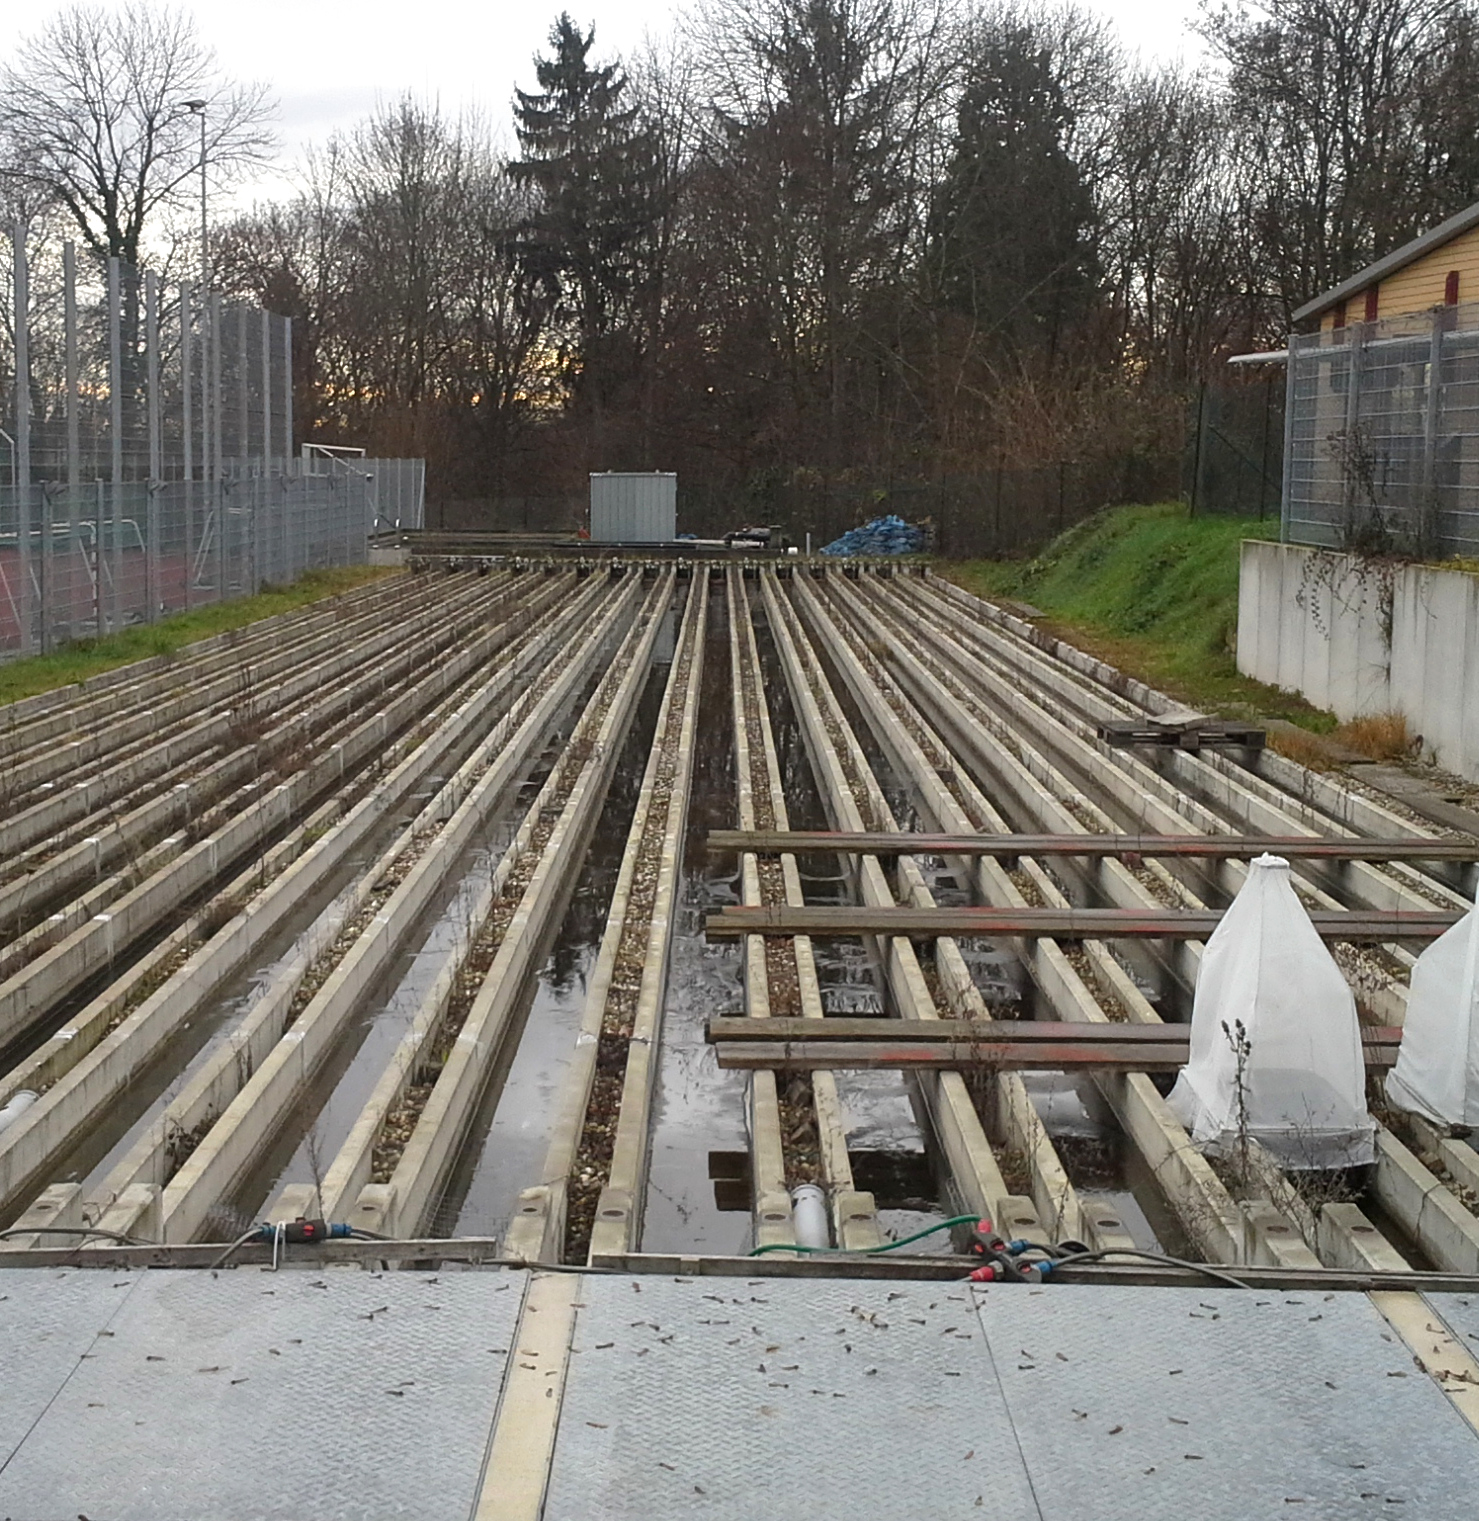
\includegraphics[width=0.9\textwidth]{figs/mesocosm_ld.jpg}
	\end{columns}

	\vfill
	\begin{columns}[T]
	\column<1->{.49\textwidth}
		\begin{itemize}
			\item Daphnia Test
			\item Lower Tier 
			\item \emph{"x out of n survived"}
		\end{itemize}

	\column<2->{.49\textwidth}
		\begin{itemize}
			\item Mesocosm
			\item Higher Tier 
			\item \emph{"number of animals"}
		\end{itemize}
	\end{columns}
\end{frame}
}%



\begin{frame}
\frametitle{Ecotoxicology is not normal}

\begin{columns}[T]
	\column{.49\textwidth}
		\center
		\begin{adjustbox}{max totalsize={0.7\textwidth}{\textheight}}
					\definecolor{myblue}{rgb}{0.137, 0.251, 0.627}
\definecolor{myalert}{rgb}{0.922, 0.482, 0.078}

% overlays etc in tikz
\tikzset{
    invisible/.style={opacity=0},
    visible on/.style={alt={#1{}{invisible}}},
    alt/.code args={<#1>#2#3}{%
      \alt<#1>{\pgfkeysalso{#2}}{\pgfkeysalso{#3}} % \pgfkeysalso doesn't change the path
    },
  }

\begin{tikzpicture}[x=1pt,y=1pt]
%\definecolor{fillColor}{RGB}{255,255,255}
%\path[use as bounding box,fill=fillColor,fill opacity=0.00] (0,0) rectangle (433.62,361.35);
\begin{scope}
\path[clip] ( 18.58, 40.74) rectangle (428.12,355.85);
\path[fill=myblue] ( 37.19, 55.07) rectangle ( 59.09, 55.07);
\path[fill=myblue] ( 80.99, 55.07) rectangle (102.89, 55.14);
\path[fill=myblue] (124.79, 55.07) rectangle (146.70, 56.05);
\path[fill=myblue] (168.60, 55.07) rectangle (190.50, 62.90);
\path[fill=myblue] (212.40, 55.07) rectangle (234.30, 94.23);
\path[fill=myblue] (256.20, 55.07) rectangle (278.10,180.39);
\path[fill=myblue] (300.00, 55.07) rectangle (321.90,305.72);
\path[fill=myblue] (343.80, 55.07) rectangle (365.70,341.53);
\path[fill=myblue] (387.60, 55.07) rectangle (409.50,198.30);
\definecolor{drawColor}{RGB}{0,0,0}
\path[draw=drawColor,line width= 0.6pt,line join=round] ( 18.58, 55.07) -- (428.12, 55.07);
\end{scope}
\begin{scope}
%\path[clip] (  0.00,  0.00) rectangle (433.62,361.35);
\definecolor{drawColor}{gray}{0.30}
\node[text=drawColor,anchor=base,inner sep=0pt, outer sep=0pt, scale=  2.50] at ( 48.14, 18.58) {0};
\node[text=drawColor,anchor=base,inner sep=0pt, outer sep=0pt, scale=  2.50] at ( 91.94, 18.58) {1};
\node[text=drawColor,anchor=base,inner sep=0pt, outer sep=0pt, scale=  2.50] at (135.74, 18.58) {2};
\node[text=drawColor,anchor=base,inner sep=0pt, outer sep=0pt, scale=  2.50] at (179.55, 18.58) {3};
\node[text=drawColor,anchor=base,inner sep=0pt, outer sep=0pt, scale=  2.50] at (223.35, 18.58) {4};
\node[text=drawColor,anchor=base,inner sep=0pt, outer sep=0pt, scale=  2.50] at (267.15, 18.58) {5};
\node[text=drawColor,anchor=base,inner sep=0pt, outer sep=0pt, scale=  2.50] at (310.95, 18.58) {6};
\node[text=drawColor,anchor=base,inner sep=0pt, outer sep=0pt, scale=  2.50] at (354.75, 18.58) {7};
\node[text=drawColor,anchor=base,inner sep=0pt, outer sep=0pt, scale=  2.50] at (398.55, 18.58) {8};
 \node[text=myalert,anchor=base,inner sep=0pt, outer sep=0pt, scale=  4, font=\bf\Huge, rotate=20,
visible on=<2->] at (218, 210) {Normal?};
\end{scope}
\end{tikzpicture}

		\end{adjustbox}
		\begin{itemize}
			\item \emph{"x out of n survived"}
			\onslide<3->{\item<ale@3-> \alert{binomial data}}
		\end{itemize}
	\column{.49\textwidth}
		\center
		\begin{adjustbox}{max totalsize={0.7\textwidth}{\textheight}}
					%\definecolor{myblue}{rgb}{0.137, 0.251, 0.627}
%\definecolor{myalert}{rgb}{0.922, 0.482, 0.078}

% overlays etc in tikz
\tikzset{
    invisible/.style={opacity=0},
    visible on/.style={alt={#1{}{invisible}}},
    alt/.code args={<#1>#2#3}{%
      \alt<#1>{\pgfkeysalso{#2}}{\pgfkeysalso{#3}} % \pgfkeysalso doesn't change the path
    },
  }


\begin{tikzpicture}[x=1pt,y=1pt]
\begin{scope}
% \path[clip] ( 18.58, 40.74) rectangle (428.12,355.85);
\path[fill=myblue] ( 37.19, 55.07) rectangle ( 71.04,198.30);
\path[fill=myblue] (104.88, 55.07) rectangle (138.73,341.53);
\path[fill=myblue] (172.58, 55.07) rectangle (206.42,341.53);
\path[fill=myblue] (240.27, 55.07) rectangle (274.12,246.04);
\path[fill=myblue] (307.96, 55.07) rectangle (341.81,150.55);
\path[fill=myblue] (375.66, 55.07) rectangle (409.50, 93.26);
\definecolor{drawColor}{RGB}{0,0,0}
\path[draw=drawColor,line width= 0.6pt,line join=round] ( 18.58, 55.07) -- (428.12, 55.07);
\end{scope}
\begin{scope}
\definecolor{drawColor}{gray}{0.30}
\node[text=drawColor,anchor=base,inner sep=0pt, outer sep=0pt, scale=  2.50] at ( 54.11, 18.58) {0};
\node[text=drawColor,anchor=base,inner sep=0pt, outer sep=0pt, scale=  2.50] at (121.81, 18.58) {1};
\node[text=drawColor,anchor=base,inner sep=0pt, outer sep=0pt, scale=  2.50] at (189.50, 18.58) {2};
\node[text=drawColor,anchor=base,inner sep=0pt, outer sep=0pt, scale=  2.50] at (257.19, 18.58) {3};
\node[text=drawColor,anchor=base,inner sep=0pt, outer sep=0pt, scale=  2.50] at (324.89, 18.58) {4};
\node[text=drawColor,anchor=base,inner sep=0pt, outer sep=0pt, scale=  2.50] at (392.58, 18.58) {5};
 \node[text=myalert,anchor=base,inner sep=0pt, outer sep=0pt, scale=  4, font=\bf\Huge, rotate=20,
visible on=<2->] at (218, 210) {Normal?};
\end{scope}
\end{tikzpicture}

		\end{adjustbox}
		\begin{itemize}
			\item \emph{"number of animals"}
			\onslide<3->{\item<ale@3-> \alert{count data}}
		\end{itemize}
	\end{columns}

	\onslide<2->{
		\Put(85,50){\begin{adjustbox}{max totalsize={0.9\textwidth}{0.4\textheight}}
			%\definecolor{myblue}{rgb}{0.137, 0.251, 0.627}
%\definecolor{myalert}{rgb}{0.922, 0.482, 0.078}

\begin{tikzpicture}[x=1pt,y=1pt]
\definecolor{fillColor}{RGB}{255,255,255}
%\path[use as bounding box,fill=fillColor,fill opacity=0.00] (0,0) rectangle (433.62,361.35);
\begin{scope}
%\path[clip] ( 18.58, 40.74) rectangle (428.12,355.85);
\path[fill=myblue] ( 37.19, 58.25) --
	( 43.40, 59.34) --
	( 49.60, 60.75) --
	( 55.81, 62.55) --
	( 62.01, 64.82) --
	( 68.22, 67.65) --
	( 74.42, 71.15) --
	( 80.63, 75.41) --
	( 86.83, 80.54) --
	( 93.04, 86.65) --
	( 99.24, 93.84) --
	(105.45,102.18) --
	(111.65,111.76) --
	(117.86,122.60) --
	(124.06,134.71) --
	(130.27,148.07) --
	(136.48,162.58) --
	(142.68,178.12) --
	(148.89,194.50) --
	(155.09,211.50) --
	(161.30,228.81) --
	(167.50,246.13) --
	(173.71,263.08) --
	(179.91,279.28) --
	(186.12,294.34) --
	(192.32,307.87) --
	(198.53,319.50) --
	(204.73,328.92) --
	(210.94,335.85) --
	(217.14,340.10) --
	(223.35,341.53) --
	(229.55,340.10) --
	(235.76,335.85) --
	(241.96,328.92) --
	(248.17,319.50) --
	(254.37,307.87) --
	(260.58,294.34) --
	(266.78,279.28) --
	(272.99,263.08) --
	(279.19,246.13) --
	(285.40,228.81) --
	(291.61,211.50) --
	(297.81,194.50) --
	(304.02,178.12) --
	(310.22,162.58) --
	(316.43,148.07) --
	(322.63,134.71) --
	(328.84,122.60) --
	(335.04,111.76) --
	(341.25,102.18) --
	(347.45, 93.84) --
	(353.66, 86.65) --
	(359.86, 80.54) --
	(366.07, 75.41) --
	(372.27, 71.15) --
	(378.48, 67.65) --
	(384.68, 64.82) --
	(390.89, 62.55) --
	(397.09, 60.75) --
	(403.30, 59.34) --
	(409.50, 58.25) --
	(409.50, 55.07) --
	(403.30, 55.07) --
	(397.09, 55.07) --
	(390.89, 55.07) --
	(384.68, 55.07) --
	(378.48, 55.07) --
	(372.27, 55.07) --
	(366.07, 55.07) --
	(359.86, 55.07) --
	(353.66, 55.07) --
	(347.45, 55.07) --
	(341.25, 55.07) --
	(335.04, 55.07) --
	(328.84, 55.07) --
	(322.63, 55.07) --
	(316.43, 55.07) --
	(310.22, 55.07) --
	(304.02, 55.07) --
	(297.81, 55.07) --
	(291.61, 55.07) --
	(285.40, 55.07) --
	(279.19, 55.07) --
	(272.99, 55.07) --
	(266.78, 55.07) --
	(260.58, 55.07) --
	(254.37, 55.07) --
	(248.17, 55.07) --
	(241.96, 55.07) --
	(235.76, 55.07) --
	(229.55, 55.07) --
	(223.35, 55.07) --
	(217.14, 55.07) --
	(210.94, 55.07) --
	(204.73, 55.07) --
	(198.53, 55.07) --
	(192.32, 55.07) --
	(186.12, 55.07) --
	(179.91, 55.07) --
	(173.71, 55.07) --
	(167.50, 55.07) --
	(161.30, 55.07) --
	(155.09, 55.07) --
	(148.89, 55.07) --
	(142.68, 55.07) --
	(136.48, 55.07) --
	(130.27, 55.07) --
	(124.06, 55.07) --
	(117.86, 55.07) --
	(111.65, 55.07) --
	(105.45, 55.07) --
	( 99.24, 55.07) --
	( 93.04, 55.07) --
	( 86.83, 55.07) --
	( 80.63, 55.07) --
	( 74.42, 55.07) --
	( 68.22, 55.07) --
	( 62.01, 55.07) --
	( 55.81, 55.07) --
	( 49.60, 55.07) --
	( 43.40, 55.07) --
	( 37.19, 55.07) --
	cycle;
\definecolor{drawColor}{RGB}{0,0,0}

\path[draw=drawColor,line width= 0.6pt,line join=round] ( 37.19, 58.25) --
	( 43.40, 59.34) --
	( 49.60, 60.75) --
	( 55.81, 62.55) --
	( 62.01, 64.82) --
	( 68.22, 67.65) --
	( 74.42, 71.15) --
	( 80.63, 75.41) --
	( 86.83, 80.54) --
	( 93.04, 86.65) --
	( 99.24, 93.84) --
	(105.45,102.18) --
	(111.65,111.76) --
	(117.86,122.60) --
	(124.06,134.71) --
	(130.27,148.07) --
	(136.48,162.58) --
	(142.68,178.12) --
	(148.89,194.50) --
	(155.09,211.50) --
	(161.30,228.81) --
	(167.50,246.13) --
	(173.71,263.08) --
	(179.91,279.28) --
	(186.12,294.34) --
	(192.32,307.87) --
	(198.53,319.50) --
	(204.73,328.92) --
	(210.94,335.85) --
	(217.14,340.10) --
	(223.35,341.53) --
	(229.55,340.10) --
	(235.76,335.85) --
	(241.96,328.92) --
	(248.17,319.50) --
	(254.37,307.87) --
	(260.58,294.34) --
	(266.78,279.28) --
	(272.99,263.08) --
	(279.19,246.13) --
	(285.40,228.81) --
	(291.61,211.50) --
	(297.81,194.50) --
	(304.02,178.12) --
	(310.22,162.58) --
	(316.43,148.07) --
	(322.63,134.71) --
	(328.84,122.60) --
	(335.04,111.76) --
	(341.25,102.18) --
	(347.45, 93.84) --
	(353.66, 86.65) --
	(359.86, 80.54) --
	(366.07, 75.41) --
	(372.27, 71.15) --
	(378.48, 67.65) --
	(384.68, 64.82) --
	(390.89, 62.55) --
	(397.09, 60.75) --
	(403.30, 59.34) --
	(409.50, 58.25);

\path[draw=drawColor,line width= 0.6pt,line join=round] ( 18.58, 55.07) -- (428.12, 55.07);
\end{scope}
\begin{scope}
%\path[clip] (  0.00,  0.00) rectangle (433.62,361.35);
\definecolor{drawColor}{gray}{0.30}
\node[text=drawColor,anchor=base,inner sep=0pt, outer sep=0pt, scale=  2.50] at ( 37.19, 18.58) {-1};
\node[text=drawColor,anchor=base,inner sep=0pt, outer sep=0pt, scale=  2.50] at ( 99.24, 18.58) {0};
\node[text=drawColor,anchor=base,inner sep=0pt, outer sep=0pt, scale=  2.50] at (161.30, 18.58) {1};
\node[text=drawColor,anchor=base,inner sep=0pt, outer sep=0pt, scale=  2.50] at (223.35, 18.58) {2};
\node[text=drawColor,anchor=base,inner sep=0pt, outer sep=0pt, scale=  2.50] at (285.40, 18.58) {3};
\node[text=drawColor,anchor=base,inner sep=0pt, outer sep=0pt, scale=  2.50] at (347.45, 18.58) {4};
\node[text=drawColor,anchor=base,inner sep=0pt, outer sep=0pt, scale=  2.50] at (409.50, 18.58) {5};

% \node[text=myalert,anchor=base,inner sep=0pt, outer sep=0pt, scale=  5, font=\bf\Huge, rotate=20] at (218, 300) {Normal?};
\end{scope}
\end{tikzpicture}

		\end{adjustbox}
		}
	}

	\vspace*{1cm}
	\begin{itemize}
		\item<4-> ignore?
		\item<5-> transform?
		\item<6-> non-parametric?
		\only<7>{\item Generalized Linear Model (GLM)}
		\only<8->{\item<ale@2-> \alert{Generalized Linear Model (GLM)}}
	\end{itemize}

\end{frame}



\begin{frame}
\frametitle{A recent history of GLM (uncomprehensive) in ecology}
	% -*- root: ../../talk.tex -*-

%%% GLM History Timeline
% see als http://stackoverflow.com/questions/217834/how-to-create-a-timeline-with-latex


% http://tex.stackexchange.com/questions/55806/mindmap-tikzpicture-in-beamer-reveal-step-by-step/55849#55849
% overlays etc in tikz
\tikzset{
    invisible/.style={opacity=0},
    visible on/.style={alt={#1{}{invisible}}},
    alt/.code args={<#1>#2#3}{%
      \alt<#1>{\pgfkeysalso{#2}}{\pgfkeysalso{#3}} % \pgfkeysalso doesn't change the path
    },
  }


\begin{tikzpicture}[scale=0.57] % timeline 1990-2010->
    % define coordinates (begin, used, end, arrow)
    \foreach \x in {2010,2011,2016, 2017}{
        \pgfmathsetlength\yearposx{(\x-1990)*1cm};
        \coordinate (y\x)   at (\yearposx,0);
        \coordinate (y\x t) at (\yearposx,+3pt);
        \coordinate (y\x b) at (\yearposx,-3pt);
    }
    % draw horizontal line with arrow
    \draw [->] (y2010) -- (y2017);
     \draw[snake] (\yearposx{(2005-1990)*1cm},0) -- (\yearposx{(2010-1990)*1cm},0);


	% Nelder
    \node [ text = myalert,
 visible on=<1>
] at (\yearposx{(2006-1990)*1cm}, 0) [rotate=90,anchor=east] {1972};
    \node [
 visible on=<2->
] at (\yearposx{(2006-1990)*1cm}, 0) [rotate=90,anchor=east] {1972};
    \node [ 
 visible on=<1>
] (nelder) at (\yearposx{(2010-1990)*1cm}, 5)  {
\includegraphics[width=10cm]{/home/edisz/Documents/work/research/projects/2016/1PHD/phd_defense/figs/tikz/glm_hist/nelder.png}};

	% oHara
    \node [ text = myalert,
 visible on=<2>
] at (\yearposx{(2010-1990)*1cm}, 0) [rotate=90,anchor=east] {2010};
    \node [ 
 visible on=<3->
] at (\yearposx{(2010-1990)*1cm}, 0) [rotate=90,anchor=east] {2010};
	\draw  [ 
 visible on=<2->
] (\yearposx{(2010-1990)*1cm}, 3pt) --  (\yearposx{(2010-1990)*1cm}, -3pt);
    \node [ 
 visible on=<2>
] (ohara) at (\yearposx{(2010-1990)*1cm}, 5)  {
\includegraphics[width=10cm]{/home/edisz/Documents/work/research/projects/2016/1PHD/phd_defense/figs/tikz/glm_hist/ohara_2010.png}};

	% warton & Hui
    \node [ text=myalert,
 visible on=<3>
] at (\yearposx{(2011-1990)*1cm}, 0) [rotate=90,anchor=east] {2011};
    \node [ 
 visible on=<4->
] at (\yearposx{(2011-1990)*1cm}, 0) [rotate=90,anchor=east] {2011};
	\draw  [ 
 visible on=<3->
] (\yearposx{(2011-1990)*1cm}, 3pt) --  (\yearposx{(2011-1990)*1cm}, -3pt);
    \node [ 
 visible on=<3>
] (ohara) at (\yearposx{(2010-1990)*1cm}, 5)  {
\includegraphics[width=10cm]{/home/edisz/Documents/work/research/projects/2016/1PHD/phd_defense/figs/tikz/glm_hist/warton_2011.png}};

	% warton mvglm
    \node [ text=myalert,
 visible on=<4>
] at (\yearposx{(2012-1990)*1cm}, 0) [rotate=90,anchor=east] {2012};
    \node [ 
 visible on=<5->
] at (\yearposx{(2012-1990)*1cm}, 0) [rotate=90,anchor=east] {2012};
	\draw  [ 
 visible on=<4->
] (\yearposx{(2012-1990)*1cm}, 3pt) --  (\yearposx{(2012-1990)*1cm}, -3pt);
    \node [ 
 visible on=<4>
] (ohara) at (\yearposx{(2010-1990)*1cm}, 5)  {
\includegraphics[width=10cm]{/home/edisz/Documents/work/research/projects/2016/1PHD/phd_defense/figs/tikz/glm_hist/warton_2012.png}};

	% Szoecs, mesocosm
    \node [ text=myalert,
 visible on=<5->
] at (\yearposx{(2015-1990)*1cm}, 0) [rotate=90,anchor=east] {2015};
	\draw  [ 
 visible on=<5->
] (\yearposx{(2015-1990)*1cm}, 3pt) --  (\yearposx{(2015-1990)*1cm}, -3pt);
    \node [ 
 visible on=<5>
] (ohara) at (\yearposx{(2010-1990)*1cm}, 5)  {
\includegraphics[width=10cm]{/home/edisz/Documents/work/research/projects/2016/1PHD/phd_defense/figs/tikz/glm_hist/Szoecs_2015.png}};

	% Szoecs, normal
    \node [ 
 visible on=<6>
] (ohara) at (\yearposx{(2010-1990)*1cm}, 5)  {
\includegraphics[width=10cm]{/home/edisz/Documents/work/research/projects/2016/1PHD/phd_defense/figs/tikz/glm_hist/Szoecs_2015_notnormal.png}};


\end{tikzpicture}

\end{frame}



\begin{frame}
\frametitle{A simulation study}

\end{frame}



\begin{frame}
\frametitle{GLMs do not always work}
	\begin{center}
		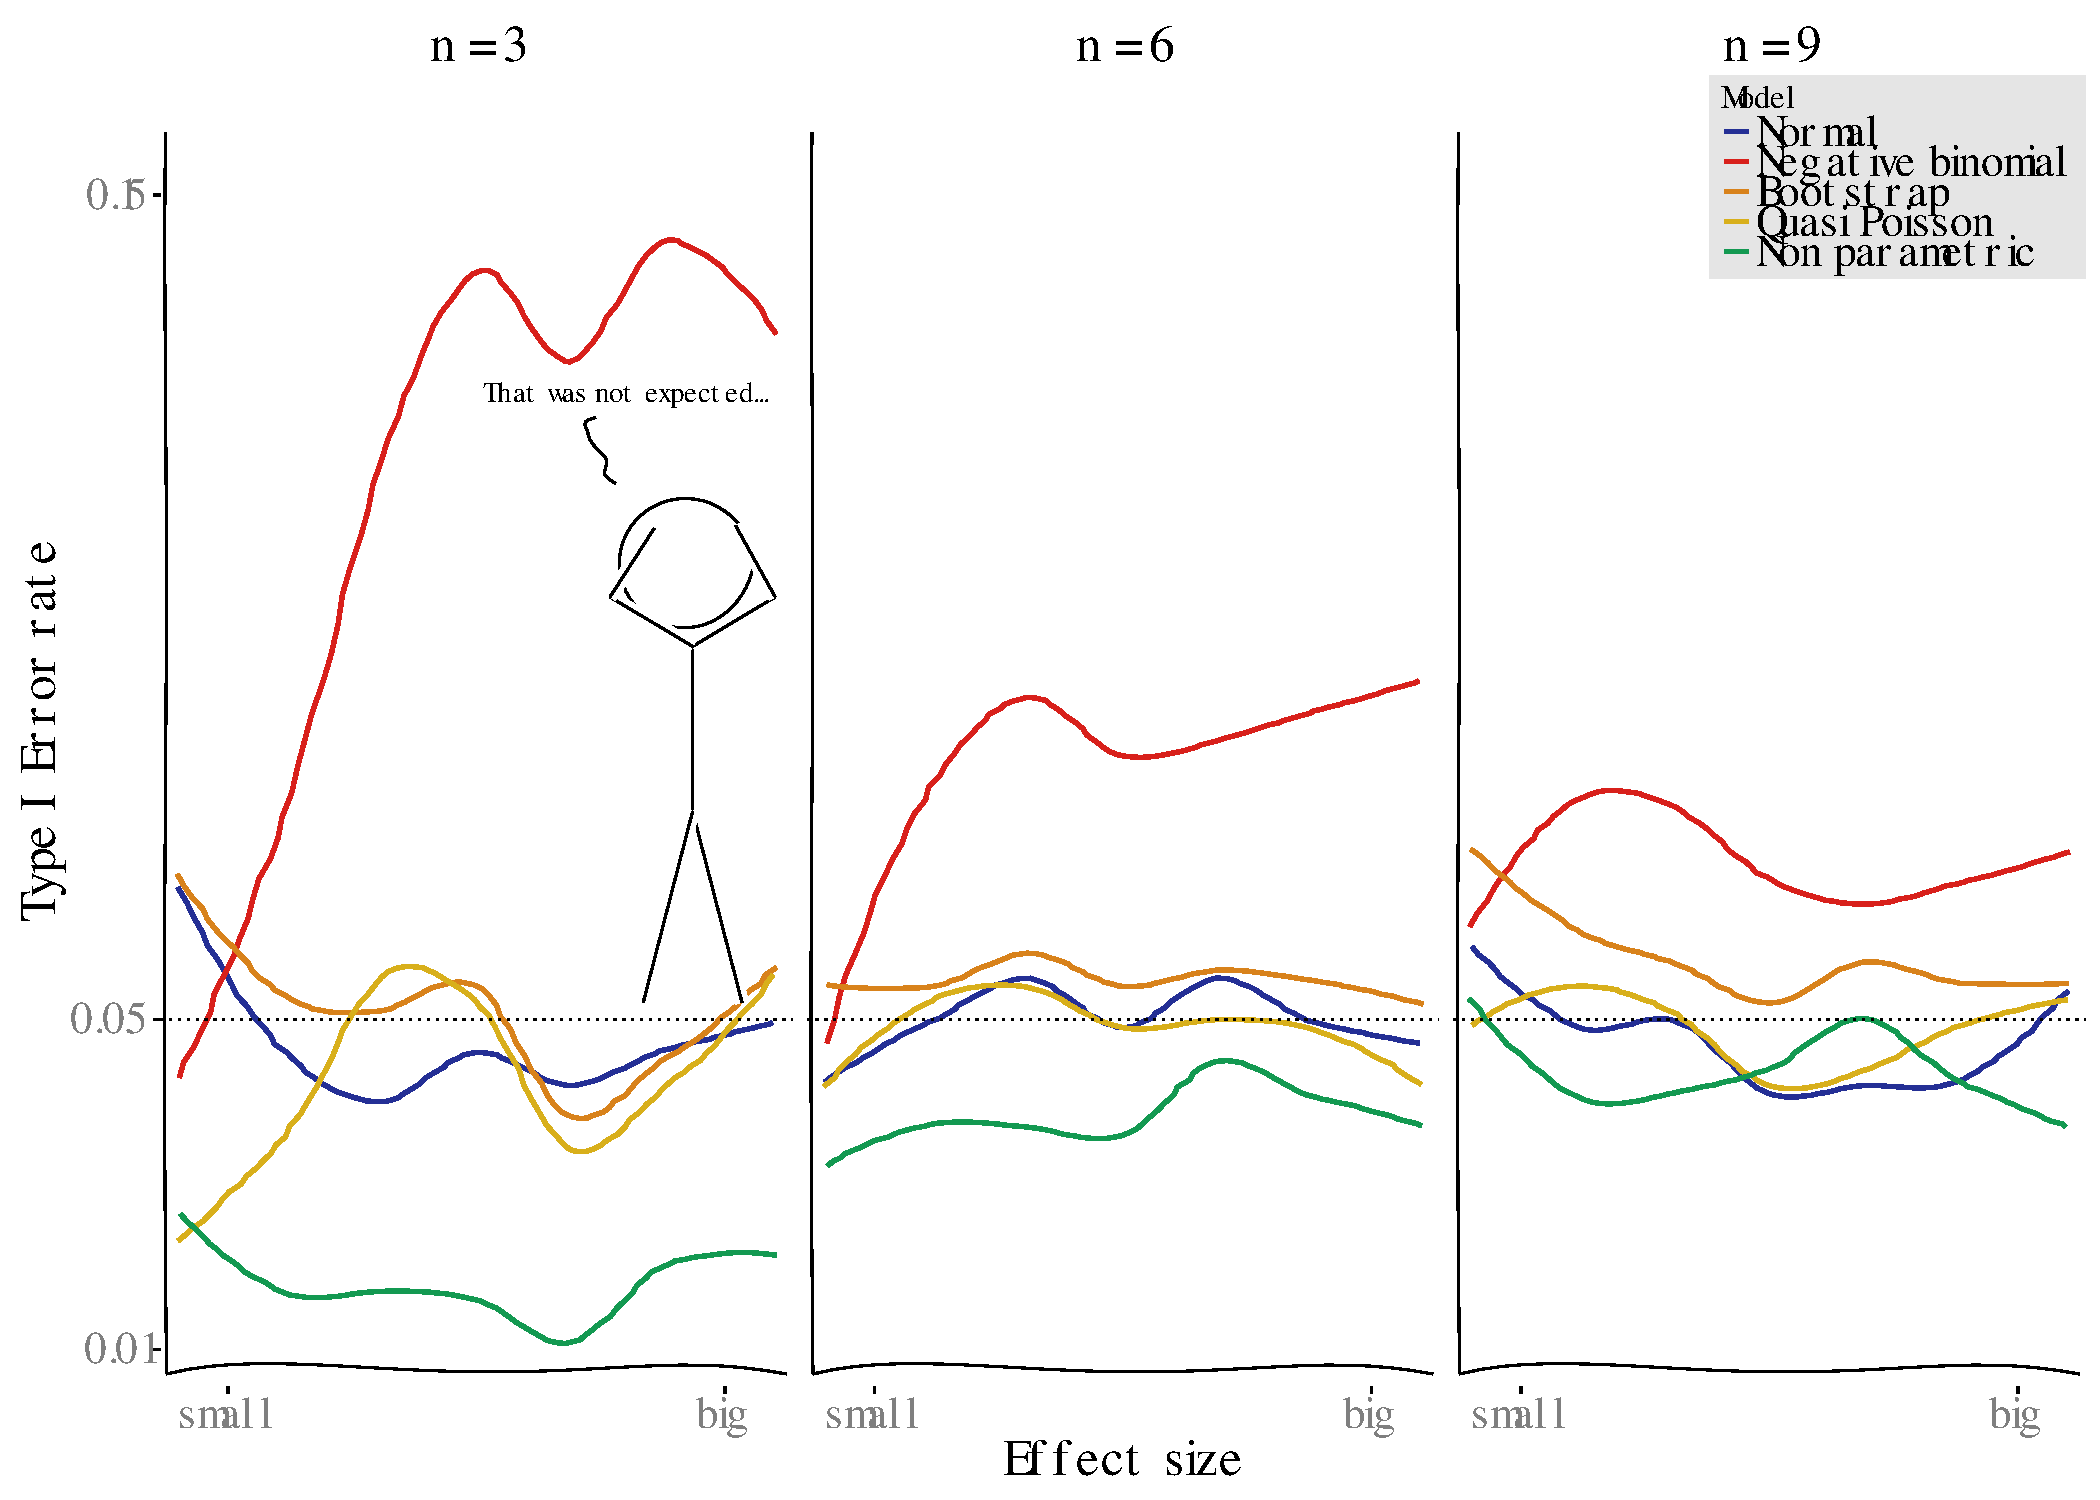
\includegraphics[width=\textwidth]{figs/p_t1_xkcd.pdf}
	\end{center}
\end{frame}


\begin{frame}
\frametitle{Power is low, GLM can do better}
	\begin{center}
	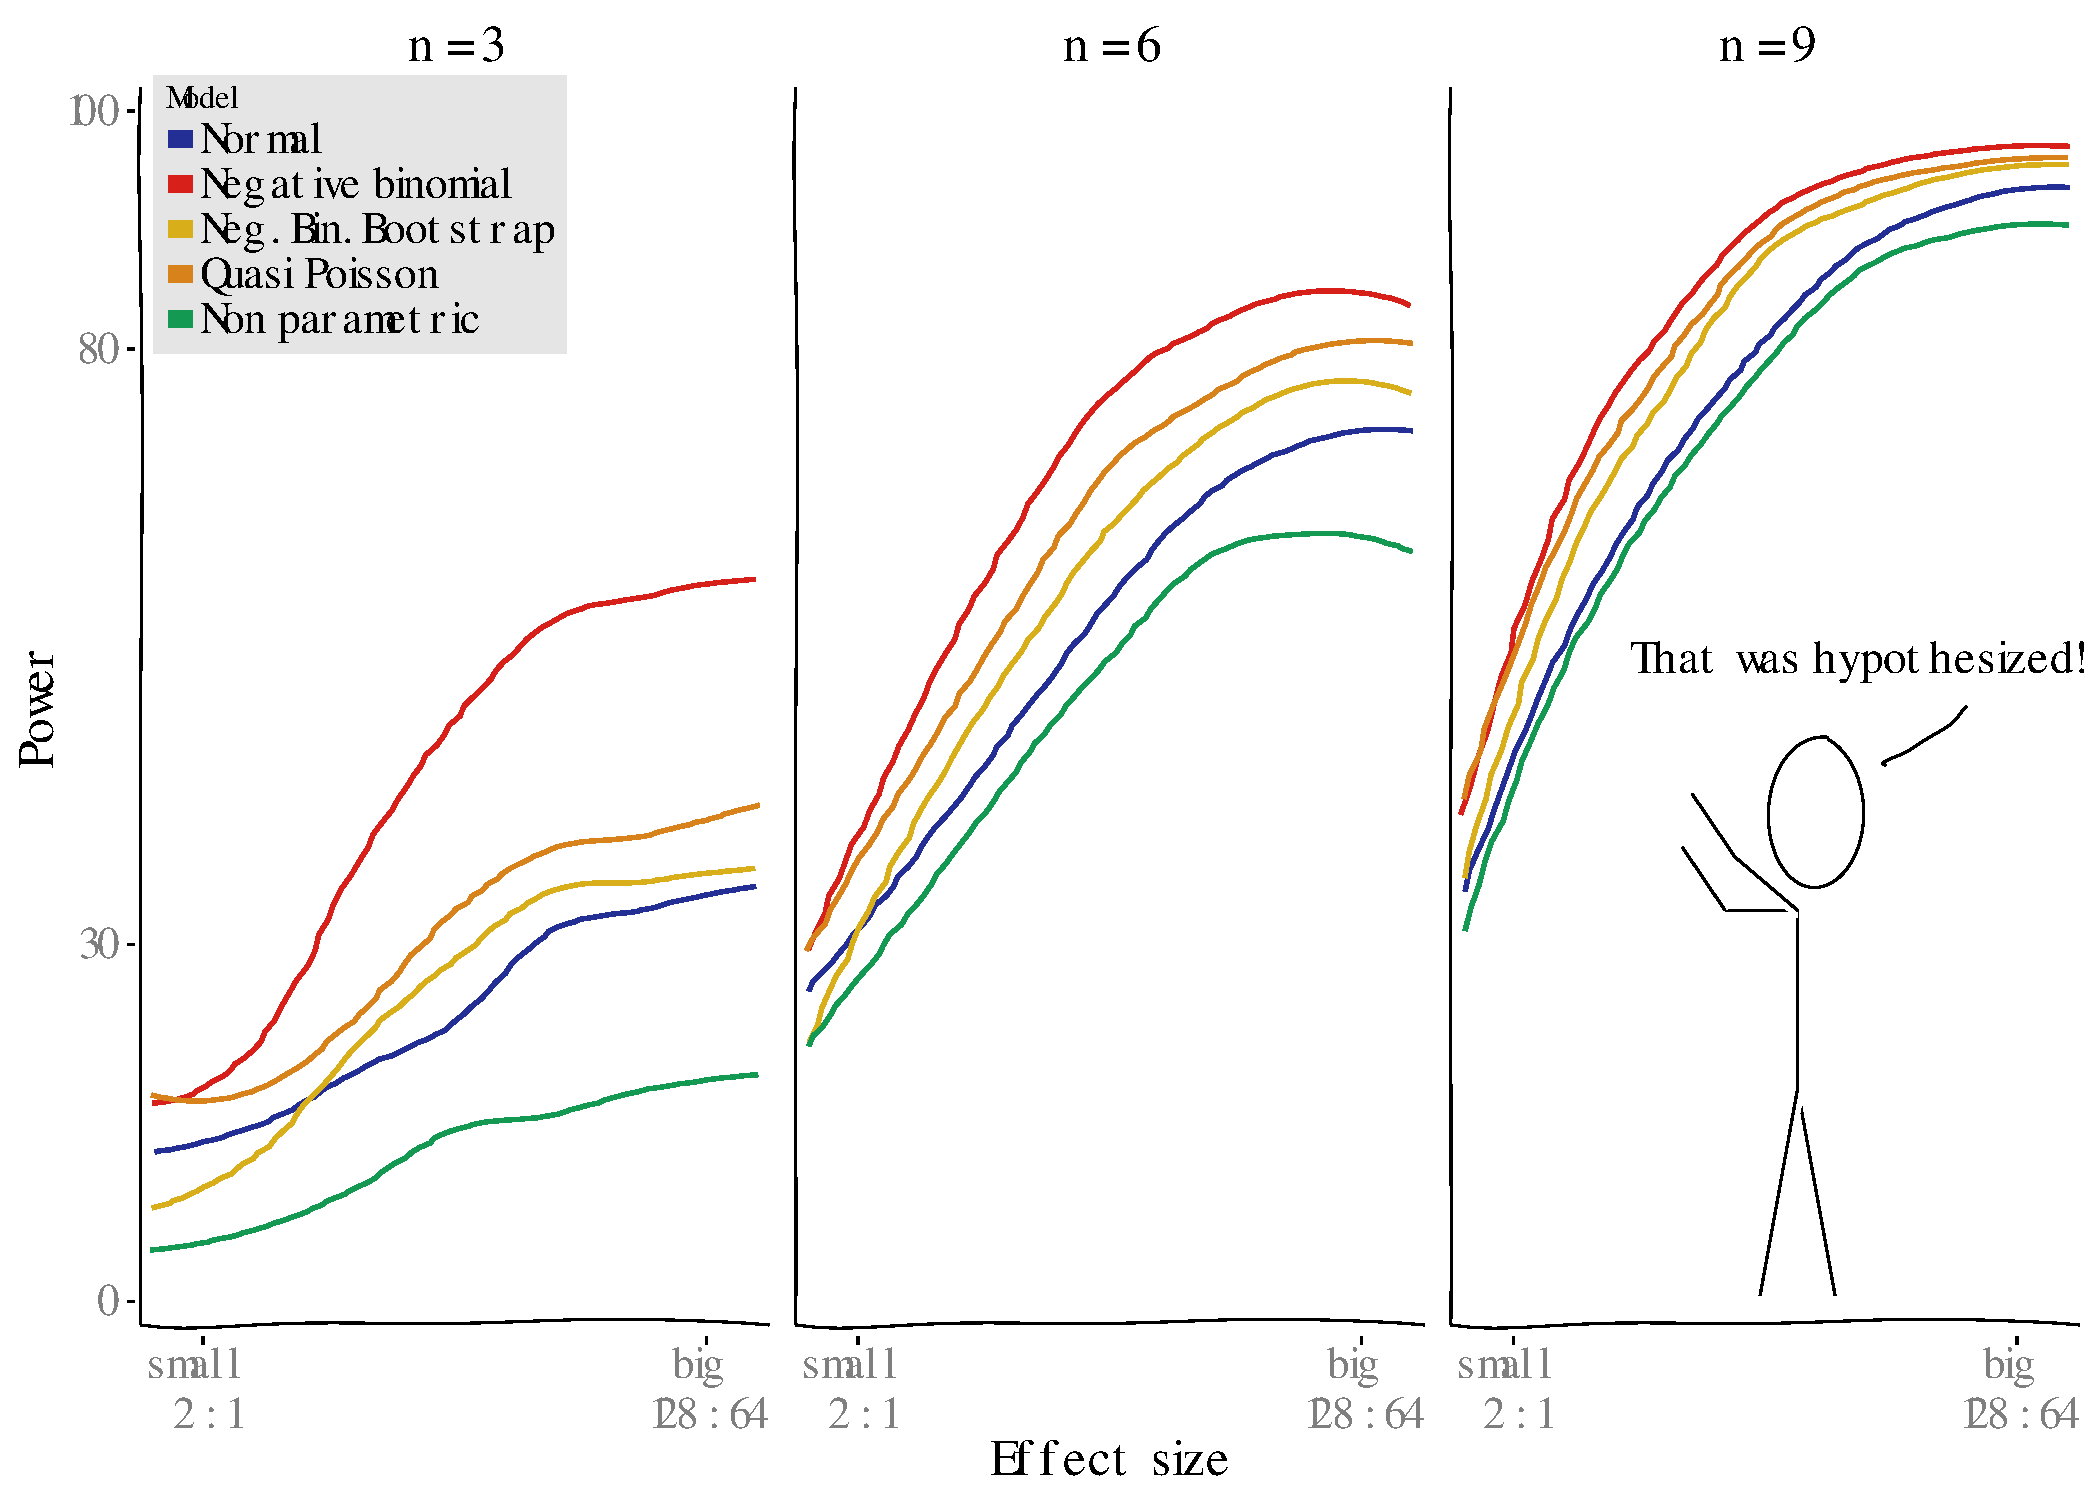
\includegraphics[width = \textwidth]{figs/p_pow_xkcd.pdf}
	\end{center}
\end{frame}



\begin{frame}
\frametitle{What we learned from this study}
	\metroset{block=fill}
		\begin{enumerate}
			\item Negative-binomial GLM show increased Type I errors
			\item Can be fixed via bootstrap
			\item Power in ecotoxicological experiments generally low
			\item NOECs are not reliable
			\item GLMs can increase this power
		\end{enumerate}
\end{frame}


\begin{frame}
\frametitle{Where are we today?}
	\only<1>{Three days earlier...}
	% -*- root: ../../talk.tex -*-

%%% GLM History Timeline
% see als http://stackoverflow.com/questions/217834/how-to-create-a-timeline-with-latex


% http://tex.stackexchange.com/questions/55806/mindmap-tikzpicture-in-beamer-reveal-step-by-step/55849#55849
% overlays etc in tikz
\tikzset{
    invisible/.style={opacity=0},
    visible on/.style={alt={#1{}{invisible}}},
    alt/.code args={<#1>#2#3}{%
      \alt<#1>{\pgfkeysalso{#2}}{\pgfkeysalso{#3}} % \pgfkeysalso doesn't change the path
    },
  }


\begin{tikzpicture}[scale=0.57] % timeline 1990-2010->
    % define coordinates (begin, used, end, arrow)
    \foreach \x in {2010,2011,2016, 2017}{
        \pgfmathsetlength\yearposx{(\x-1990)*1cm};
        \coordinate (y\x)   at (\yearposx,0);
        \coordinate (y\x t) at (\yearposx,+3pt);
        \coordinate (y\x b) at (\yearposx,-3pt);
    }
    % draw horizontal line with arrow
    \draw [->] (y2010) -- (y2017);
     \draw[snake] (\yearposx{(2005-1990)*1cm},0) -- (\yearposx{(2010-1990)*1cm},0);

	% Nelder
    \node [ 
 visible on=<1->
] at (\yearposx{(2006-1990)*1cm}, 0) [rotate=90,anchor=east] {1972};

	% oHara
    \node [ 
 visible on=<1->
] at (\yearposx{(2010-1990)*1cm}, 0) [rotate=90,anchor=east] {2010};
	\draw  [ 
 visible on=<1->
] (\yearposx{(2010-1990)*1cm}, 3pt) --  (\yearposx{(2010-1990)*1cm}, -3pt);


	% warton & Hui
    \node [ 
 visible on=<1->
] at (\yearposx{(2011-1990)*1cm}, 0) [rotate=90,anchor=east] {2011};
	\draw  [ 
 visible on=<1->
] (\yearposx{(2011-1990)*1cm}, 3pt) --  (\yearposx{(2011-1990)*1cm}, -3pt);

	% warton mvglm
    \node [ 
 visible on=<1->
] at (\yearposx{(2012-1990)*1cm}, 0) [rotate=90,anchor=east] {2012};
	\draw  [ 
 visible on=<1->
] (\yearposx{(2012-1990)*1cm}, 3pt) --  (\yearposx{(2012-1990)*1cm}, -3pt);

	% Szoecs, mesocosm
    \node [ text = myalert,
 visible on=<1>
] at (\yearposx{(2015-1990)*1cm}, 0) [rotate=90,anchor=east] {2015};
    \node [
 visible on=<2->
] at (\yearposx{(2015-1990)*1cm}, 0) [rotate=90,anchor=east] {2015};
	\draw  [ 
 visible on=<1->
] (\yearposx{(2015-1990)*1cm}, 3pt) --  (\yearposx{(2015-1990)*1cm}, -3pt);

	% Ives
    \node [ 
 visible on=<1>
] (ohara) at (\yearposx{(2010-1990)*1cm}, 5)  {
\includegraphics[width=10cm]{/home/edisz/Documents/work/research/projects/2016/1PHD/phd_defense/figs/tikz/glm_hist/ives_2015.png}};

	% warton
    \node [ text = myalert,
 visible on=<2->
] at (\yearposx{(2016-1990)*1cm}, 0) [rotate=90,anchor=east] {2016};
	\draw  [ 
 visible on=<2->
] (\yearposx{(2016-1990)*1cm}, 3pt) --  (\yearposx{(2016-1990)*1cm}, -3pt);
    \node [ 
 visible on=<2->
] (ohara) at (\yearposx{(2010-1990)*1cm}, 5)  {
\includegraphics[width=10cm]{/home/edisz/Documents/work/research/projects/2016/1PHD/phd_defense/figs/tikz/glm_hist/warton_2016.png}};


\end{tikzpicture}

\end{frame}


{%
\setbeamertemplate{frame footer}{Warton, D.I., Lyons, M., Stoklosa, J., Ives, A.R., 2016. Three points to consider when choosing a LM or GLM test for count data. Methods in Ecology and Evolution 7, 882–890.
}
\begin{frame}
\frametitle{Where are we today?}
	% \metroset{block=fill}
	\begin{exampleblock}{Three points to consider ...}
		\begin{enumerate}
			\item Choose your model based on data properties
			\item Fix Type I errors by resampling
			\item Models that better fit the data have better power properties
		\end{enumerate}
	\end{exampleblock}
\end{frame}
}

%%% ---------------------------------------------------------------------------
\section{Exploring Monitoring Data for ERA}

\begin{frame}
\frametitle{Environmental Monitoring}

\end{frame}

\begin{frame}
\frametitle{Overview on data compiled}

\end{frame}

\begin{frame}
\frametitle{Thresholds}

\end{frame}

\begin{frame}
\frametitle{Statistics with chemical measurements}

\end{frame}


\begin{frame}
\frametitle{Dynamics}

\end{frame}


\begin{frame}
\frametitle{Risks}
Check: What did go wrong with Neonics during ERA?
Exposure wromg? Effect wrong (e.g. did not consider sensitive species)?
=> Quite sure that Effect assessment missed it...
=> show SSD, highlighting standard test species (from EPA)
* old guidance document did not enforce insect.
* new one (from 2013) enforces additional insect data

RAC is landscape dependend (=> exposure?)

Example for power (experimental setup)

\end{frame}


\begin{frame}
\frametitle{What we learned}

\end{frame}

%%% ---------------------------------------------------------------------------
\section{Solutions for Linking Data in ERA}

\begin{frame}
\frametitle{Biologists \& Chemists face the same problems}
	\small
	\centering
	\textbf{\alert{\underline{Names}}}
	\begin{columns}[t]
	\column{.45\textwidth}
	\emph{Osmia rufa, Osmia bicornis, Osmia ruffa, Osmia unilandauis, Osmia spec.} 
	\column{.45\textwidth}
	Chlorpyrifos, Chlorpyriphos, Chlorphyrifos, Chlorpyrifos-ethyl, Chlorpypifot
	\end{columns}
	\pause

	\centering
	\textbf{\alert{\underline{Hierarchies}}}
	\begin{columns}[t]
	\column{.45\textwidth}
	Hymenoptera/ Apoidea/ Megachilidae/ Osmia/ rufa 
	\column{.45\textwidth}
	organophospate, ester, insecticide
	\end{columns}
	\pause

	\centering
	\textbf{\alert{\underline{Traits / Properties}}}
	\begin{columns}[t]
	\column{.45\textwidth}
	Wing length, Mass, Season 
	\column{.45\textwidth}
	Mass, $K_{OW}$, $LC_{50}$
	\end{columns}
	\pause

	\centering
	\textbf{\alert{\underline{Identifiers}}}
	\begin{columns}[t]
	\column{.45\textwidth}
	NCBI, ITIS, EOL, ... 
	\column{.45\textwidth}
	2921-88-2, Clc1c(OP(=S)[...], InChI=1S/C9H11C[...], SBPBAQFW[...], CSID,...
	\end{columns}
	\vspace{0.8em}
	\pause

	\rule{\textwidth}{1pt}
	\textbf{\alert{\underline{Amount of data}}}

	\begin{columns}[t]
	\column{.45\textwidth}
	\centering
	2993 taxa
	\column{.45\textwidth}
	\centering
	489 pesticides \\ (+ 590 other organics)
	\end{columns}
\end{frame}


{%
\setbeamertemplate{frame footer}{Münch et al. (2016). DoOR 2.0 - Comprehensive Mapping of Drosophila melanogaster Odorant Responses. Scientific Reports 6, 21841
}
\begin{frame}{}
\frametitle{Instead of wasting time...}
... use \alert{webchem}! \\
	\hspace*{2cm}
	\begin{adjustbox}{max totalsize={\textwidth}{0.8\textheight}}
				% -*- root: ../../talk.tex -*-

\definecolor{blue}{RGB}{32, 126, 153}
\definecolor{green}{RGB}{33, 182, 78}
\definecolor{red}{RGB}{246, 72, 45}
\definecolor{orange}{RGB}{246, 146, 45}
\definecolor{yellow}{RGB}{180, 180, 18}

\begin{tikzpicture}[node distance = 0.2cm, auto]

%styles
\tikzstyle{circ} = [circle, draw, text = black,   line width=1pt, 
    text width=4cm, text centered, scale=1, font=\bf\huge]
\tikzstyle{rect} = [rectangle, draw, text = black, line width=1pt,
    text width=5cm, text centered, rounded corners, minimum height=1.5cm, minimum width=1cm, font=\bf\huge]

\tikzstyle{line} = [draw, -{Latex[length=5mm,width=3mm]}, line width=1mm, opacity = 0.8]

    % input nodes
    \node [circ, fill=green] (cas_i) {CAS};
    \node  (name_i) [circ, below=of cas_i, fill = blue] {Name};
    \node  (inchikey_i) [circ, below=of name_i, fill = red] {InChiKey};
    \node  (other_i) [circ, below=of inchikey_i, fill =orange] {Other};
   
   % source nodes
   \node (cir) [rect, right=of cas_i, shift={(13,7)}, fill = yellow]{CIR};
   \node (chemspider) [rect, below=1cm of cir, fill = yellow]{ChemSpider};
   \node (cts) [rect, below=1cm of chemspider, fill = yellow]{CTS};
   \node (etox) [rect, below=1cm of cts, fill = yellow]{ETOX};
   \node (chemid) [rect, below=1cm of etox, fill = yellow]{ChemID};
  \node (opsin) [rect, below=1cm of chemid, fill = yellow]{OPSIN};
  \node (alan) [rect, below=1cm of opsin, fill = yellow]{Pesticide Compendium};
  \node (wiki) [rect, below=1cm of alan, fill = yellow]{wikidata};
  \node (pubchem) [rect, below=1cm of wiki, fill = yellow]{PubChem};
  \node (pan) [rect, below=1cm of pubchem, fill = yellow]{PAN};
  \node (src) [rect, below=1cm of pan, fill = yellow]{SRC};

	% output nodes
    \node (cas_o) [circ, right=of cir, shift={(15,-5)}, , fill =green] {CAS};
    \node  (name_o) [circ, below=of cas_o, , fill =blue] {Name};
    \node  (inchikey_o) [circ, below=of name_o, fill =red] {InChiKey \\ InChi};
    \node  (smiles_o) [circ, below=of inchikey_o, fill =red] {SMILES};
    \node  (legis_o) [circ, below=of smiles_o, fill =orange] {Legislation};
    \node  (syno_o) [circ, below=of legis_o, fill =orange] {Synonyms};
    \node  (other_o) [circ, below=of syno_o, fill =orange] {Other};
    \node (prop_o) [circ, above=of cas_o, fill =orange] {Properties};
    \node (tox_o) [circ, above=of prop_o, fill =orange] {Toxicology};

    %paths
   % from cas_i
    \path [line, green] (cas_i.east) -- (cir.west);
    \path [line, green] (cas_i.east) -- (chemspider.west);
    \path [line, green] (cas_i.east) -- (cts.west);
    \path [line, green] (cas_i.east) -- (etox.west);
    \path [line, green] (cas_i.east) -- (chemid.west);
    \path [line, green] (cas_i.east) -- (alan.west);
    \path [line, green] (cas_i.east) -- (wiki.west);
    \path [line, green] (cas_i.east) -- (pubchem.west);
    \path [line, green] (cas_i.east) -- (pan.west);
    \path [line, green] (cas_i.east) -- (src.west);

	% from name_i
    \path [line, blue] (name_i.east) -- (cir.west);
    \path [line, blue] (name_i.east) -- (chemspider.west);
    \path [line, blue] (name_i.east) -- (cts.west);
    \path [line, blue] (name_i.east) -- (etox.west);
    \path [line, blue] (name_i.east) -- (chemid.west);
    \path [line, blue] (name_i.east) -- (opsin.west);
    \path [line, blue] (name_i.east) -- (alan.west);
    \path [line, blue] (name_i.east) -- (wiki.west);
    \path [line, blue] (name_i.east) -- (pubchem.west);
    \path [line, blue] (name_i.east) -- (pan.west);

    %from inchikey_i
    \path [line, red] (inchikey_i.east) -- (cir.west);
    \path [line, red] (inchikey_i.east) -- (chemspider.west);
    \path [line, red] (inchikey_i.east) -- (cts.west);
    \path [line, red] (inchikey_i.east) -- (chemid.west);
    \path [line, red] (inchikey_i.east) -- (wiki.west);
    \path [line, red] (inchikey_i.east) -- (pubchem.west);
   
    %from other_i
    \path [line, orange] (other_i.east) -- (cir.west);
    \path [line, orange] (other_i.east) -- (chemspider.west);
    \path [line, orange] (other_i.east) -- (cts.west);
    \path [line, orange] (other_i.east) -- (etox.west);
    \path [line, orange] (other_i.east) -- (wiki.west);
    \path [line, orange] (other_i.east) -- (pubchem.west);

   %from cir
  \path [line, orange] (cir.east) -- (prop_o.west);
  \path [line, green] (cir.east) -- (cas_o.west);
  \path [line, blue] (cir.east) -- (name_o.west);
  \path [line, red] (cir.east) -- (inchikey_o.west);
  \path [line, red] (cir.east) -- (smiles_o.west);
  \path [line, orange] (cir.east) -- (other_o.west);

  %from chemspider
  \path [line, orange] (chemspider.east) -- (prop_o.west);
  \path [line, blue] (chemspider.east) -- (name_o.west);
  \path [line, red] (chemspider.east) -- (inchikey_o.west);
  \path [line, red] (chemspider.east) -- (smiles_o.west);

  % from cts
  \path [line, blue] (cts.east) -- (name_o.west);
  \path [line, green] (cts.east) -- (cas_o.west);
  \path [line, red] (cts.east) -- (inchikey_o.west);
  \path [line, red] (cts.east) -- (smiles_o.west);
  \path [line, orange] (cts.east) -- (syno_o.west);
  \path [line, orange] (cts.east) -- (other_o.west);

	% from etox
   \path [line, orange] (etox.east) -- (tox_o.west);
   \path [line, green] (etox.east) -- (cas_o.west);
   \path [line, blue] (etox.east) -- (name_o.west);
   \path [line, orange] (etox.east) -- (legis_o.west);
   \path [line, orange] (etox.east) -- (syno_o.west);
   \path [line, orange] (etox.east) -- (other_o.west);

  %from chemid
   \path [line, orange] (chemid.east) -- (tox_o.west);
   \path [line, orange] (chemid.east) -- (prop_o.west);
   \path [line, green] (chemid.east) -- (cas_o.west);
   \path [line, blue] (chemid.east) -- (name_o.west);
   \path [line, red] (chemid.east) -- (inchikey_o.west);
   \path [line, red] (chemid.east) -- (smiles_o.west);
   \path [line, orange] (chemid.east) -- (syno_o.west);

	%from opsin
    \path [line, green] (opsin.east) -- (cas_o.west);
   \path [line, red] (opsin.east) -- (inchikey_o.west);
   \path [line, red] (opsin.east) -- (smiles_o.west);

   %from alan wood
   \path [line, green] (alan.east) -- (cas_o.west);
   \path [line, blue] (alan.east) -- (name_o.west);
   \path [line, red] (alan.east) -- (inchikey_o.west);
   \path [line, orange] (alan.east) -- (other_o.west);

  %from wiki
   \path [line, green] (wiki.east) -- (cas_o.west);
   \path [line, red] (wiki.east) -- (inchikey_o.west);
   \path [line, red] (wiki.east) -- (smiles_o.west);
   \path [line, orange] (wiki.east) -- (other_o.west);

  % from pubchem
     \path [line, orange] (pubchem.east) -- (prop_o.west);
     \path [line, blue] (pubchem.east) -- (name_o.west);
     \path [line, red] (pubchem.east) -- (inchikey_o.west);
     \path [line, red] (pubchem.east) -- (smiles_o.west);
     \path [line, orange] (pubchem.east) -- (syno_o.west);

    % from pan
    \path [line, orange] (pan.east) -- (tox_o.west);
    \path [line, orange] (pan.east) -- (prop_o.west);
     \path [line, blue] (pan.east) -- (name_o.west);
   \path [line, green] (pan.east) -- (cas_o.west);
   \path [line, orange] (pan.east) -- (legis_o.west);
   \path [line, orange] (pan.east) -- (other_o.west);

  %from src
       \path [line, orange] (src.east) -- (tox_o.west);
     \path [line, blue] (src.east) -- (name_o.west);
   \path [line, green] (src.east) -- (cas_o.west);

\end{tikzpicture}

	\end{adjustbox}

\pause
\vspace*{-1cm}\emph{''\alert{webchem} ...likely saved hundreds of working hours''}
\end{frame}
}


{%
\setbeamertemplate{frame footer}{Dr. Susan E. Johnston, University of Edinburgh. On twitter.
}
\begin{frame}
\frametitle{Instead of wasting time...}
... use \alert{taxize!} \\
	\hspace*{-2cm}
	\begin{center}
	
\includegraphics[height=0.6\textheight]{figs/sources_taxize.png}
	\end{center}

\pause
\emph{''Days of searching done during my morning coffee. Amazing. \alert{taxize}.''}
\end{frame}
}



%%% ---------------------------------------------------------------------------
\section*{Recap}

\begin{frame}
\frametitle{What we learned}
	\metroset{block=fill}
	\begin{exampleblock}{\checkmark Improving Statistics in ERA}
		\begin{itemize}
			\item Change your model, not your data
			\item Ultimately ban NOEC
			\item Take LOQ into account
		\end{itemize}
	\end{exampleblock}

\pause
	\begin{exampleblock}{\checkmark Exploring Monitoring Data for ERA}
		\begin{itemize}
			\item Risk drivers and dynamics
			\item Agricultural Small streams at risk \& neglected
			\item Neonicotinoids
			\item Feedback for ERA
		\end{itemize}
	\end{exampleblock}

\pause
	\begin{exampleblock}{\checkmark Solutions for Linking Data in ERA}
		\begin{itemize}
			\item Handling big eco(toxico-)logical data not easy
			\item Now easier
		\end{itemize}
	\end{exampleblock}


\end{frame}


%%% ---------------------------------------------------------------------------
%%% Final slide
\begin{frame}[standout]
	\frametitle{}

	\vspace{1em}
	\Huge{Statistical Ecotoxicology} \\[0.3em]
	\large{Improving the Utilisation of Data for \\ Environmental Risk Assessment} \\[1em]

	\normalsize
	Eduard Szöcs \\[3em]

	\faLaptop~~~\textbf{\href{http://edild.github.io/}{http://edild.github.io/ }}\\[.5em]
	\faTwitter~~~\textbf{\href{http://twitter.com/EduardSzoecs}{@EduardSzoecs}} 	\\[0.5em]
	\faFilePowerpointO~~~\textbf{\href{https://github.com/edild/phd_defense}{https://github.com/edild/phd\_defense}}\\[0.5em]
	\faBook~~~\textbf{\href{https://github.com/edild/phd_thesis}{https://github.com/edild/phd\_thesis}}\\[3em]

	\begin{center}\ccbysa\end{center} 

\end{frame}


\appendix

\begin{frame}
\frametitle{Power en detail}
	\begin{adjustbox}{max totalsize={\textwidth}{\textheight}}
				% Created by tikzDevice version 0.10.1 on 2016-12-15 15:38:57
% !TEX encoding = UTF-8 Unicode
\begin{tikzpicture}[x=1pt,y=1pt]
\definecolor{fillColor}{RGB}{255,255,255}
\path[use as bounding box,fill=fillColor,fill opacity=0.00] (0,0) rectangle (1011.78,722.70);
\begin{scope}
\path[clip] (  3.50,423.03) rectangle (1011.78,722.70);
\definecolor{drawColor}{RGB}{255,255,255}
\definecolor{fillColor}{RGB}{255,255,255}

\path[draw=drawColor,line width= 0.6pt,line join=round,line cap=round,fill=fillColor] (  3.50,423.03) rectangle (1011.78,722.70);
\end{scope}
\begin{scope}
\path[clip] ( 66.13,444.26) rectangle (374.35,689.45);
\definecolor{fillColor}{RGB}{255,255,255}

\path[fill=fillColor] ( 66.13,444.26) rectangle (374.35,689.45);
\definecolor{drawColor}{gray}{0.90}

\path[draw=drawColor,line width= 0.6pt,line join=round] ( 66.13,450.69) --
	(374.35,450.69);

\path[draw=drawColor,line width= 0.6pt,line join=round] ( 66.13,530.26) --
	(374.35,530.26);

\path[draw=drawColor,line width= 0.6pt,line join=round] ( 66.13,564.52) --
	(374.35,564.52);

\path[draw=drawColor,line width= 0.6pt,line join=round] ( 66.13,598.79) --
	(374.35,598.79);

\path[draw=drawColor,line width= 0.6pt,line join=round] ( 66.13,633.06) --
	(374.35,633.06);

\path[draw=drawColor,line width= 0.6pt,line join=round] ( 66.13,653.10) --
	(374.35,653.10);

\path[draw=drawColor,line width= 0.6pt,line join=round] ( 66.13,667.32) --
	(374.35,667.32);

\path[draw=drawColor,line width= 0.6pt,line join=round] ( 66.13,678.35) --
	(374.35,678.35);

\path[draw=drawColor,line width= 0.6pt,line join=round] ( 80.14,444.26) --
	( 80.14,689.45);

\path[draw=drawColor,line width= 0.6pt,line join=round] (126.84,444.26) --
	(126.84,689.45);

\path[draw=drawColor,line width= 0.6pt,line join=round] (173.54,444.26) --
	(173.54,689.45);

\path[draw=drawColor,line width= 0.6pt,line join=round] (220.24,444.26) --
	(220.24,689.45);

\path[draw=drawColor,line width= 0.6pt,line join=round] (266.94,444.26) --
	(266.94,689.45);

\path[draw=drawColor,line width= 0.6pt,line join=round] (313.64,444.26) --
	(313.64,689.45);

\path[draw=drawColor,line width= 0.6pt,line join=round] (360.34,444.26) --
	(360.34,689.45);
\definecolor{drawColor}{RGB}{0,0,0}

\path[draw=drawColor,line width= 0.6pt,line join=round] ( 80.14,543.98) --
	(126.84,527.20) --
	(173.54,519.23) --
	(220.24,526.14) --
	(266.94,521.64) --
	(313.64,529.26) --
	(360.34,529.26);

\path[draw=drawColor,line width= 0.6pt,dash pattern=on 2pt off 2pt ,line join=round] ( 80.14,524.93) --
	(126.84,543.29) --
	(173.54,571.78) --
	(220.24,581.39) --
	(266.94,577.49) --
	(313.64,586.51) --
	(360.34,577.54);

\path[draw=drawColor,line width= 0.6pt,dash pattern=on 4pt off 2pt ,line join=round] ( 80.14,545.46) --
	(126.84,532.20) --
	(173.54,531.24) --
	(220.24,534.06) --
	(266.94,516.69) --
	(313.64,531.24) --
	(360.34,534.97);

\path[draw=drawColor,line width= 0.6pt,dash pattern=on 4pt off 4pt ,line join=round] ( 80.14,495.87) --
	(126.84,501.78) --
	(173.54,534.58) --
	(220.24,532.18) --
	(266.94,511.19) --
	(313.64,528.24) --
	(360.34,534.11);

\path[draw=drawColor,line width= 0.6pt,dash pattern=on 1pt off 3pt ,line join=round] ( 80.14,600.97) --
	(126.84,629.07) --
	(173.54,651.76) --
	(220.24,669.62) --
	(266.94,675.19) --
	(313.64,677.71) --
	(360.34,678.30);

\path[draw=drawColor,line width= 0.6pt,dash pattern=on 1pt off 3pt on 4pt off 3pt ,line join=round] ( 80.14,499.80) --
	(126.84,470.74) --
	(173.54,476.93) --
	(220.24,473.93) --
	(266.94,455.41) --
	(313.64,497.93) --
	(360.34,484.96);
\definecolor{fillColor}{RGB}{0,0,0}

\path[fill=fillColor] ( 80.14,543.98) circle (  4.64);

\path[draw=drawColor,line width= 0.4pt,line join=round,line cap=round] ( 80.14,532.14) --
	( 86.39,521.32) --
	( 73.89,521.32) --
	( 80.14,532.14);

\path[draw=drawColor,line width= 0.4pt,line join=round,line cap=round] ( 75.50,540.82) -- ( 84.78,550.10);

\path[draw=drawColor,line width= 0.4pt,line join=round,line cap=round] ( 75.50,550.10) -- ( 84.78,540.82);

\path[draw=drawColor,line width= 0.4pt,line join=round,line cap=round] ( 75.50,491.23) rectangle ( 84.78,500.51);

\path[draw=drawColor,line width= 0.4pt,line join=round,line cap=round] ( 80.14,600.97) circle (  4.64);

\path[fill=fillColor] ( 80.14,507.01) --
	( 86.39,496.19) --
	( 73.89,496.19) --
	cycle;

\path[fill=fillColor] (126.84,527.20) circle (  4.64);

\path[draw=drawColor,line width= 0.4pt,line join=round,line cap=round] (126.84,550.51) --
	(133.09,539.69) --
	(120.59,539.69) --
	(126.84,550.51);

\path[draw=drawColor,line width= 0.4pt,line join=round,line cap=round] (122.20,527.56) -- (131.48,536.84);

\path[draw=drawColor,line width= 0.4pt,line join=round,line cap=round] (122.20,536.84) -- (131.48,527.56);

\path[draw=drawColor,line width= 0.4pt,line join=round,line cap=round] (122.20,497.14) rectangle (131.48,506.42);

\path[draw=drawColor,line width= 0.4pt,line join=round,line cap=round] (126.84,629.07) circle (  4.64);

\path[fill=fillColor] (126.84,477.95) --
	(133.09,467.13) --
	(120.59,467.13) --
	cycle;

\path[fill=fillColor] (173.54,519.23) circle (  4.64);

\path[draw=drawColor,line width= 0.4pt,line join=round,line cap=round] (173.54,579.00) --
	(179.79,568.17) --
	(167.29,568.17) --
	(173.54,579.00);

\path[draw=drawColor,line width= 0.4pt,line join=round,line cap=round] (168.90,526.60) -- (178.18,535.88);

\path[draw=drawColor,line width= 0.4pt,line join=round,line cap=round] (168.90,535.88) -- (178.18,526.60);

\path[draw=drawColor,line width= 0.4pt,line join=round,line cap=round] (168.90,529.94) rectangle (178.18,539.22);

\path[draw=drawColor,line width= 0.4pt,line join=round,line cap=round] (173.54,651.76) circle (  4.64);

\path[fill=fillColor] (173.54,484.14) --
	(179.79,473.32) --
	(167.29,473.32) --
	cycle;

\path[fill=fillColor] (220.24,526.14) circle (  4.64);

\path[draw=drawColor,line width= 0.4pt,line join=round,line cap=round] (220.24,588.61) --
	(226.49,577.79) --
	(213.99,577.79) --
	(220.24,588.61);

\path[draw=drawColor,line width= 0.4pt,line join=round,line cap=round] (215.60,529.42) -- (224.88,538.70);

\path[draw=drawColor,line width= 0.4pt,line join=round,line cap=round] (215.60,538.70) -- (224.88,529.42);

\path[draw=drawColor,line width= 0.4pt,line join=round,line cap=round] (215.60,527.55) rectangle (224.88,536.82);

\path[draw=drawColor,line width= 0.4pt,line join=round,line cap=round] (220.24,669.62) circle (  4.64);

\path[fill=fillColor] (220.24,481.14) --
	(226.49,470.32) --
	(213.99,470.32) --
	cycle;

\path[fill=fillColor] (266.94,521.64) circle (  4.64);

\path[draw=drawColor,line width= 0.4pt,line join=round,line cap=round] (266.94,584.71) --
	(273.19,573.89) --
	(260.69,573.89) --
	(266.94,584.71);

\path[draw=drawColor,line width= 0.4pt,line join=round,line cap=round] (262.30,512.05) -- (271.58,521.33);

\path[draw=drawColor,line width= 0.4pt,line join=round,line cap=round] (262.30,521.33) -- (271.58,512.05);

\path[draw=drawColor,line width= 0.4pt,line join=round,line cap=round] (262.30,506.55) rectangle (271.58,515.83);

\path[draw=drawColor,line width= 0.4pt,line join=round,line cap=round] (266.94,675.19) circle (  4.64);

\path[fill=fillColor] (266.94,462.62) --
	(273.19,451.80) --
	(260.69,451.80) --
	cycle;

\path[fill=fillColor] (313.64,529.26) circle (  4.64);

\path[draw=drawColor,line width= 0.4pt,line join=round,line cap=round] (313.64,593.72) --
	(319.89,582.90) --
	(307.39,582.90) --
	(313.64,593.72);

\path[draw=drawColor,line width= 0.4pt,line join=round,line cap=round] (309.00,526.60) -- (318.28,535.88);

\path[draw=drawColor,line width= 0.4pt,line join=round,line cap=round] (309.00,535.88) -- (318.28,526.60);

\path[draw=drawColor,line width= 0.4pt,line join=round,line cap=round] (309.00,523.60) rectangle (318.28,532.88);

\path[draw=drawColor,line width= 0.4pt,line join=round,line cap=round] (313.64,677.71) circle (  4.64);

\path[fill=fillColor] (313.64,505.15) --
	(319.89,494.32) --
	(307.39,494.32) --
	cycle;

\path[fill=fillColor] (360.34,529.26) circle (  4.64);

\path[draw=drawColor,line width= 0.4pt,line join=round,line cap=round] (360.34,584.76) --
	(366.59,573.94) --
	(354.09,573.94) --
	(360.34,584.76);

\path[draw=drawColor,line width= 0.4pt,line join=round,line cap=round] (355.70,530.33) -- (364.98,539.61);

\path[draw=drawColor,line width= 0.4pt,line join=round,line cap=round] (355.70,539.61) -- (364.98,530.33);

\path[draw=drawColor,line width= 0.4pt,line join=round,line cap=round] (355.70,529.47) rectangle (364.98,538.75);

\path[draw=drawColor,line width= 0.4pt,line join=round,line cap=round] (360.34,678.30) circle (  4.64);

\path[fill=fillColor] (360.34,492.18) --
	(366.59,481.35) --
	(354.09,481.35) --
	cycle;

\path[draw=drawColor,line width= 0.6pt,dash pattern=on 4pt off 4pt ,line join=round] ( 66.13,530.26) -- (374.35,530.26);

\path[draw=drawColor,line width= 0.6pt,dash pattern=on 4pt off 4pt ,line join=round] ( 66.13,530.26) -- (374.35,530.26);

\path[draw=drawColor,line width= 0.6pt,dash pattern=on 4pt off 4pt ,line join=round] ( 66.13,530.26) -- (374.35,530.26);

\path[draw=drawColor,line width= 0.6pt,dash pattern=on 4pt off 4pt ,line join=round] ( 66.13,530.26) -- (374.35,530.26);

\path[draw=drawColor,line width= 0.6pt,dash pattern=on 4pt off 4pt ,line join=round] ( 66.13,530.26) -- (374.35,530.26);

\path[draw=drawColor,line width= 0.6pt,dash pattern=on 4pt off 4pt ,line join=round] ( 66.13,530.26) -- (374.35,530.26);

\path[draw=drawColor,line width= 0.6pt,dash pattern=on 4pt off 4pt ,line join=round] ( 66.13,530.26) -- (374.35,530.26);

\path[draw=drawColor,line width= 0.6pt,dash pattern=on 4pt off 4pt ,line join=round] ( 66.13,530.26) -- (374.35,530.26);

\path[draw=drawColor,line width= 0.6pt,dash pattern=on 4pt off 4pt ,line join=round] ( 66.13,530.26) -- (374.35,530.26);

\path[draw=drawColor,line width= 0.6pt,dash pattern=on 4pt off 4pt ,line join=round] ( 66.13,530.26) -- (374.35,530.26);

\path[draw=drawColor,line width= 0.6pt,dash pattern=on 4pt off 4pt ,line join=round] ( 66.13,530.26) -- (374.35,530.26);

\path[draw=drawColor,line width= 0.6pt,dash pattern=on 4pt off 4pt ,line join=round] ( 66.13,530.26) -- (374.35,530.26);

\path[draw=drawColor,line width= 0.6pt,dash pattern=on 4pt off 4pt ,line join=round] ( 66.13,530.26) -- (374.35,530.26);

\path[draw=drawColor,line width= 0.6pt,dash pattern=on 4pt off 4pt ,line join=round] ( 66.13,530.26) -- (374.35,530.26);

\path[draw=drawColor,line width= 0.6pt,dash pattern=on 4pt off 4pt ,line join=round] ( 66.13,530.26) -- (374.35,530.26);

\path[draw=drawColor,line width= 0.6pt,dash pattern=on 4pt off 4pt ,line join=round] ( 66.13,530.26) -- (374.35,530.26);

\path[draw=drawColor,line width= 0.6pt,dash pattern=on 4pt off 4pt ,line join=round] ( 66.13,530.26) -- (374.35,530.26);

\path[draw=drawColor,line width= 0.6pt,dash pattern=on 4pt off 4pt ,line join=round] ( 66.13,530.26) -- (374.35,530.26);

\path[draw=drawColor,line width= 0.6pt,dash pattern=on 4pt off 4pt ,line join=round] ( 66.13,530.26) -- (374.35,530.26);

\path[draw=drawColor,line width= 0.6pt,dash pattern=on 4pt off 4pt ,line join=round] ( 66.13,530.26) -- (374.35,530.26);

\path[draw=drawColor,line width= 0.6pt,dash pattern=on 4pt off 4pt ,line join=round] ( 66.13,530.26) -- (374.35,530.26);

\path[draw=drawColor,line width= 0.6pt,dash pattern=on 4pt off 4pt ,line join=round] ( 66.13,530.26) -- (374.35,530.26);

\path[draw=drawColor,line width= 0.6pt,dash pattern=on 4pt off 4pt ,line join=round] ( 66.13,530.26) -- (374.35,530.26);

\path[draw=drawColor,line width= 0.6pt,dash pattern=on 4pt off 4pt ,line join=round] ( 66.13,530.26) -- (374.35,530.26);

\path[draw=drawColor,line width= 0.6pt,dash pattern=on 4pt off 4pt ,line join=round] ( 66.13,530.26) -- (374.35,530.26);

\path[draw=drawColor,line width= 0.6pt,dash pattern=on 4pt off 4pt ,line join=round] ( 66.13,530.26) -- (374.35,530.26);

\path[draw=drawColor,line width= 0.6pt,dash pattern=on 4pt off 4pt ,line join=round] ( 66.13,530.26) -- (374.35,530.26);

\path[draw=drawColor,line width= 0.6pt,dash pattern=on 4pt off 4pt ,line join=round] ( 66.13,530.26) -- (374.35,530.26);

\path[draw=drawColor,line width= 0.6pt,dash pattern=on 4pt off 4pt ,line join=round] ( 66.13,530.26) -- (374.35,530.26);

\path[draw=drawColor,line width= 0.6pt,dash pattern=on 4pt off 4pt ,line join=round] ( 66.13,530.26) -- (374.35,530.26);

\path[draw=drawColor,line width= 0.6pt,dash pattern=on 4pt off 4pt ,line join=round] ( 66.13,530.26) -- (374.35,530.26);

\path[draw=drawColor,line width= 0.6pt,dash pattern=on 4pt off 4pt ,line join=round] ( 66.13,530.26) -- (374.35,530.26);

\path[draw=drawColor,line width= 0.6pt,dash pattern=on 4pt off 4pt ,line join=round] ( 66.13,530.26) -- (374.35,530.26);

\path[draw=drawColor,line width= 0.6pt,dash pattern=on 4pt off 4pt ,line join=round] ( 66.13,530.26) -- (374.35,530.26);

\path[draw=drawColor,line width= 0.6pt,dash pattern=on 4pt off 4pt ,line join=round] ( 66.13,530.26) -- (374.35,530.26);

\path[draw=drawColor,line width= 0.6pt,dash pattern=on 4pt off 4pt ,line join=round] ( 66.13,530.26) -- (374.35,530.26);

\path[draw=drawColor,line width= 0.6pt,dash pattern=on 4pt off 4pt ,line join=round] ( 66.13,530.26) -- (374.35,530.26);

\path[draw=drawColor,line width= 0.6pt,dash pattern=on 4pt off 4pt ,line join=round] ( 66.13,530.26) -- (374.35,530.26);

\path[draw=drawColor,line width= 0.6pt,dash pattern=on 4pt off 4pt ,line join=round] ( 66.13,530.26) -- (374.35,530.26);

\path[draw=drawColor,line width= 0.6pt,dash pattern=on 4pt off 4pt ,line join=round] ( 66.13,530.26) -- (374.35,530.26);

\path[draw=drawColor,line width= 0.6pt,dash pattern=on 4pt off 4pt ,line join=round] ( 66.13,530.26) -- (374.35,530.26);

\path[draw=drawColor,line width= 0.6pt,dash pattern=on 4pt off 4pt ,line join=round] ( 66.13,530.26) -- (374.35,530.26);
\definecolor{drawColor}{gray}{0.50}

\path[draw=drawColor,line width= 0.6pt,line join=round,line cap=round] ( 66.13,444.26) rectangle (374.35,689.45);
\end{scope}
\begin{scope}
\path[clip] (381.35,444.26) rectangle (689.56,689.45);
\definecolor{fillColor}{RGB}{255,255,255}

\path[fill=fillColor] (381.35,444.26) rectangle (689.56,689.45);
\definecolor{drawColor}{gray}{0.90}

\path[draw=drawColor,line width= 0.6pt,line join=round] (381.35,450.69) --
	(689.56,450.69);

\path[draw=drawColor,line width= 0.6pt,line join=round] (381.35,530.26) --
	(689.56,530.26);

\path[draw=drawColor,line width= 0.6pt,line join=round] (381.35,564.52) --
	(689.56,564.52);

\path[draw=drawColor,line width= 0.6pt,line join=round] (381.35,598.79) --
	(689.56,598.79);

\path[draw=drawColor,line width= 0.6pt,line join=round] (381.35,633.06) --
	(689.56,633.06);

\path[draw=drawColor,line width= 0.6pt,line join=round] (381.35,653.10) --
	(689.56,653.10);

\path[draw=drawColor,line width= 0.6pt,line join=round] (381.35,667.32) --
	(689.56,667.32);

\path[draw=drawColor,line width= 0.6pt,line join=round] (381.35,678.35) --
	(689.56,678.35);

\path[draw=drawColor,line width= 0.6pt,line join=round] (395.36,444.26) --
	(395.36,689.45);

\path[draw=drawColor,line width= 0.6pt,line join=round] (442.06,444.26) --
	(442.06,689.45);

\path[draw=drawColor,line width= 0.6pt,line join=round] (488.76,444.26) --
	(488.76,689.45);

\path[draw=drawColor,line width= 0.6pt,line join=round] (535.46,444.26) --
	(535.46,689.45);

\path[draw=drawColor,line width= 0.6pt,line join=round] (582.16,444.26) --
	(582.16,689.45);

\path[draw=drawColor,line width= 0.6pt,line join=round] (628.85,444.26) --
	(628.85,689.45);

\path[draw=drawColor,line width= 0.6pt,line join=round] (675.55,444.26) --
	(675.55,689.45);
\definecolor{drawColor}{RGB}{0,0,0}

\path[draw=drawColor,line width= 0.6pt,line join=round] (395.36,522.80) --
	(442.06,527.20) --
	(488.76,534.97) --
	(535.46,529.26) --
	(582.16,534.97) --
	(628.85,526.14) --
	(675.55,528.24);

\path[draw=drawColor,line width= 0.6pt,dash pattern=on 2pt off 2pt ,line join=round] (395.36,527.44) --
	(442.06,551.29) --
	(488.76,558.76) --
	(535.46,554.71) --
	(582.16,555.90) --
	(628.85,558.20) --
	(675.55,559.86);

\path[draw=drawColor,line width= 0.6pt,dash pattern=on 4pt off 2pt ,line join=round] (395.36,534.97) --
	(442.06,531.24) --
	(488.76,537.59) --
	(535.46,534.06) --
	(582.16,535.86) --
	(628.85,534.06) --
	(675.55,532.20);

\path[draw=drawColor,line width= 0.6pt,dash pattern=on 4pt off 4pt ,line join=round] (395.36,521.44) --
	(442.06,532.26) --
	(488.76,534.06) --
	(535.46,529.26) --
	(582.16,530.26) --
	(628.85,529.26) --
	(675.55,521.64);

\path[draw=drawColor,line width= 0.6pt,dash pattern=on 1pt off 3pt ,line join=round] (395.36,599.28) --
	(442.06,627.29) --
	(488.76,651.85) --
	(535.46,667.01) --
	(582.16,675.29) --
	(628.85,677.56) --
	(675.55,678.20);

\path[draw=drawColor,line width= 0.6pt,dash pattern=on 1pt off 3pt on 4pt off 3pt ,line join=round] (395.36,508.20) --
	(442.06,516.69) --
	(488.76,515.37) --
	(535.46,514.02) --
	(582.16,525.05) --
	(628.85,515.37) --
	(675.55,516.69);
\definecolor{fillColor}{RGB}{0,0,0}

\path[fill=fillColor] (395.36,522.80) circle (  4.64);

\path[draw=drawColor,line width= 0.4pt,line join=round,line cap=round] (395.36,534.66) --
	(401.61,523.84) --
	(389.11,523.84) --
	(395.36,534.66);

\path[draw=drawColor,line width= 0.4pt,line join=round,line cap=round] (390.72,530.33) -- (400.00,539.61);

\path[draw=drawColor,line width= 0.4pt,line join=round,line cap=round] (390.72,539.61) -- (400.00,530.33);

\path[draw=drawColor,line width= 0.4pt,line join=round,line cap=round] (390.72,516.80) rectangle (400.00,526.08);

\path[draw=drawColor,line width= 0.4pt,line join=round,line cap=round] (395.36,599.28) circle (  4.64);

\path[fill=fillColor] (395.36,515.41) --
	(401.61,504.59) --
	(389.11,504.59) --
	cycle;

\path[fill=fillColor] (442.06,527.20) circle (  4.64);

\path[draw=drawColor,line width= 0.4pt,line join=round,line cap=round] (442.06,558.51) --
	(448.31,547.68) --
	(435.81,547.68) --
	(442.06,558.51);

\path[draw=drawColor,line width= 0.4pt,line join=round,line cap=round] (437.42,526.60) -- (446.70,535.88);

\path[draw=drawColor,line width= 0.4pt,line join=round,line cap=round] (437.42,535.88) -- (446.70,526.60);

\path[draw=drawColor,line width= 0.4pt,line join=round,line cap=round] (437.42,527.63) rectangle (446.70,536.90);

\path[draw=drawColor,line width= 0.4pt,line join=round,line cap=round] (442.06,627.29) circle (  4.64);

\path[fill=fillColor] (442.06,523.91) --
	(448.31,513.08) --
	(435.81,513.08) --
	cycle;

\path[fill=fillColor] (488.76,534.97) circle (  4.64);

\path[draw=drawColor,line width= 0.4pt,line join=round,line cap=round] (488.76,565.98) --
	(495.01,555.16) --
	(482.51,555.16) --
	(488.76,565.98);

\path[draw=drawColor,line width= 0.4pt,line join=round,line cap=round] (484.12,532.96) -- (493.40,542.23);

\path[draw=drawColor,line width= 0.4pt,line join=round,line cap=round] (484.12,542.23) -- (493.40,532.96);

\path[draw=drawColor,line width= 0.4pt,line join=round,line cap=round] (484.12,529.42) rectangle (493.40,538.70);

\path[draw=drawColor,line width= 0.4pt,line join=round,line cap=round] (488.76,651.85) circle (  4.64);

\path[fill=fillColor] (488.76,522.59) --
	(495.01,511.76) --
	(482.51,511.76) --
	cycle;

\path[fill=fillColor] (535.46,529.26) circle (  4.64);

\path[draw=drawColor,line width= 0.4pt,line join=round,line cap=round] (535.46,561.93) --
	(541.70,551.11) --
	(529.21,551.11) --
	(535.46,561.93);

\path[draw=drawColor,line width= 0.4pt,line join=round,line cap=round] (530.82,529.42) -- (540.10,538.70);

\path[draw=drawColor,line width= 0.4pt,line join=round,line cap=round] (530.82,538.70) -- (540.10,529.42);

\path[draw=drawColor,line width= 0.4pt,line join=round,line cap=round] (530.82,524.62) rectangle (540.10,533.90);

\path[draw=drawColor,line width= 0.4pt,line join=round,line cap=round] (535.46,667.01) circle (  4.64);

\path[fill=fillColor] (535.46,521.23) --
	(541.70,510.41) --
	(529.21,510.41) --
	cycle;

\path[fill=fillColor] (582.16,534.97) circle (  4.64);

\path[draw=drawColor,line width= 0.4pt,line join=round,line cap=round] (582.16,563.12) --
	(588.40,552.30) --
	(575.91,552.30) --
	(582.16,563.12);

\path[draw=drawColor,line width= 0.4pt,line join=round,line cap=round] (577.52,531.22) -- (586.79,540.50);

\path[draw=drawColor,line width= 0.4pt,line join=round,line cap=round] (577.52,540.50) -- (586.79,531.22);

\path[draw=drawColor,line width= 0.4pt,line join=round,line cap=round] (577.52,525.62) rectangle (586.79,534.90);

\path[draw=drawColor,line width= 0.4pt,line join=round,line cap=round] (582.16,675.29) circle (  4.64);

\path[fill=fillColor] (582.16,532.26) --
	(588.40,521.44) --
	(575.91,521.44) --
	cycle;

\path[fill=fillColor] (628.85,526.14) circle (  4.64);

\path[draw=drawColor,line width= 0.4pt,line join=round,line cap=round] (628.85,565.42) --
	(635.10,554.60) --
	(622.61,554.60) --
	(628.85,565.42);

\path[draw=drawColor,line width= 0.4pt,line join=round,line cap=round] (624.22,529.42) -- (633.49,538.70);

\path[draw=drawColor,line width= 0.4pt,line join=round,line cap=round] (624.22,538.70) -- (633.49,529.42);

\path[draw=drawColor,line width= 0.4pt,line join=round,line cap=round] (624.22,524.62) rectangle (633.49,533.90);

\path[draw=drawColor,line width= 0.4pt,line join=round,line cap=round] (628.85,677.56) circle (  4.64);

\path[fill=fillColor] (628.85,522.59) --
	(635.10,511.76) --
	(622.61,511.76) --
	cycle;

\path[fill=fillColor] (675.55,528.24) circle (  4.64);

\path[draw=drawColor,line width= 0.4pt,line join=round,line cap=round] (675.55,567.08) --
	(681.80,556.25) --
	(669.31,556.25) --
	(675.55,567.08);

\path[draw=drawColor,line width= 0.4pt,line join=round,line cap=round] (670.91,527.56) -- (680.19,536.84);

\path[draw=drawColor,line width= 0.4pt,line join=round,line cap=round] (670.91,536.84) -- (680.19,527.56);

\path[draw=drawColor,line width= 0.4pt,line join=round,line cap=round] (670.91,517.00) rectangle (680.19,526.28);

\path[draw=drawColor,line width= 0.4pt,line join=round,line cap=round] (675.55,678.20) circle (  4.64);

\path[fill=fillColor] (675.55,523.91) --
	(681.80,513.08) --
	(669.31,513.08) --
	cycle;

\path[draw=drawColor,line width= 0.6pt,dash pattern=on 4pt off 4pt ,line join=round] (381.35,530.26) -- (689.56,530.26);

\path[draw=drawColor,line width= 0.6pt,dash pattern=on 4pt off 4pt ,line join=round] (381.35,530.26) -- (689.56,530.26);

\path[draw=drawColor,line width= 0.6pt,dash pattern=on 4pt off 4pt ,line join=round] (381.35,530.26) -- (689.56,530.26);

\path[draw=drawColor,line width= 0.6pt,dash pattern=on 4pt off 4pt ,line join=round] (381.35,530.26) -- (689.56,530.26);

\path[draw=drawColor,line width= 0.6pt,dash pattern=on 4pt off 4pt ,line join=round] (381.35,530.26) -- (689.56,530.26);

\path[draw=drawColor,line width= 0.6pt,dash pattern=on 4pt off 4pt ,line join=round] (381.35,530.26) -- (689.56,530.26);

\path[draw=drawColor,line width= 0.6pt,dash pattern=on 4pt off 4pt ,line join=round] (381.35,530.26) -- (689.56,530.26);

\path[draw=drawColor,line width= 0.6pt,dash pattern=on 4pt off 4pt ,line join=round] (381.35,530.26) -- (689.56,530.26);

\path[draw=drawColor,line width= 0.6pt,dash pattern=on 4pt off 4pt ,line join=round] (381.35,530.26) -- (689.56,530.26);

\path[draw=drawColor,line width= 0.6pt,dash pattern=on 4pt off 4pt ,line join=round] (381.35,530.26) -- (689.56,530.26);

\path[draw=drawColor,line width= 0.6pt,dash pattern=on 4pt off 4pt ,line join=round] (381.35,530.26) -- (689.56,530.26);

\path[draw=drawColor,line width= 0.6pt,dash pattern=on 4pt off 4pt ,line join=round] (381.35,530.26) -- (689.56,530.26);

\path[draw=drawColor,line width= 0.6pt,dash pattern=on 4pt off 4pt ,line join=round] (381.35,530.26) -- (689.56,530.26);

\path[draw=drawColor,line width= 0.6pt,dash pattern=on 4pt off 4pt ,line join=round] (381.35,530.26) -- (689.56,530.26);

\path[draw=drawColor,line width= 0.6pt,dash pattern=on 4pt off 4pt ,line join=round] (381.35,530.26) -- (689.56,530.26);

\path[draw=drawColor,line width= 0.6pt,dash pattern=on 4pt off 4pt ,line join=round] (381.35,530.26) -- (689.56,530.26);

\path[draw=drawColor,line width= 0.6pt,dash pattern=on 4pt off 4pt ,line join=round] (381.35,530.26) -- (689.56,530.26);

\path[draw=drawColor,line width= 0.6pt,dash pattern=on 4pt off 4pt ,line join=round] (381.35,530.26) -- (689.56,530.26);

\path[draw=drawColor,line width= 0.6pt,dash pattern=on 4pt off 4pt ,line join=round] (381.35,530.26) -- (689.56,530.26);

\path[draw=drawColor,line width= 0.6pt,dash pattern=on 4pt off 4pt ,line join=round] (381.35,530.26) -- (689.56,530.26);

\path[draw=drawColor,line width= 0.6pt,dash pattern=on 4pt off 4pt ,line join=round] (381.35,530.26) -- (689.56,530.26);

\path[draw=drawColor,line width= 0.6pt,dash pattern=on 4pt off 4pt ,line join=round] (381.35,530.26) -- (689.56,530.26);

\path[draw=drawColor,line width= 0.6pt,dash pattern=on 4pt off 4pt ,line join=round] (381.35,530.26) -- (689.56,530.26);

\path[draw=drawColor,line width= 0.6pt,dash pattern=on 4pt off 4pt ,line join=round] (381.35,530.26) -- (689.56,530.26);

\path[draw=drawColor,line width= 0.6pt,dash pattern=on 4pt off 4pt ,line join=round] (381.35,530.26) -- (689.56,530.26);

\path[draw=drawColor,line width= 0.6pt,dash pattern=on 4pt off 4pt ,line join=round] (381.35,530.26) -- (689.56,530.26);

\path[draw=drawColor,line width= 0.6pt,dash pattern=on 4pt off 4pt ,line join=round] (381.35,530.26) -- (689.56,530.26);

\path[draw=drawColor,line width= 0.6pt,dash pattern=on 4pt off 4pt ,line join=round] (381.35,530.26) -- (689.56,530.26);

\path[draw=drawColor,line width= 0.6pt,dash pattern=on 4pt off 4pt ,line join=round] (381.35,530.26) -- (689.56,530.26);

\path[draw=drawColor,line width= 0.6pt,dash pattern=on 4pt off 4pt ,line join=round] (381.35,530.26) -- (689.56,530.26);

\path[draw=drawColor,line width= 0.6pt,dash pattern=on 4pt off 4pt ,line join=round] (381.35,530.26) -- (689.56,530.26);

\path[draw=drawColor,line width= 0.6pt,dash pattern=on 4pt off 4pt ,line join=round] (381.35,530.26) -- (689.56,530.26);

\path[draw=drawColor,line width= 0.6pt,dash pattern=on 4pt off 4pt ,line join=round] (381.35,530.26) -- (689.56,530.26);

\path[draw=drawColor,line width= 0.6pt,dash pattern=on 4pt off 4pt ,line join=round] (381.35,530.26) -- (689.56,530.26);

\path[draw=drawColor,line width= 0.6pt,dash pattern=on 4pt off 4pt ,line join=round] (381.35,530.26) -- (689.56,530.26);

\path[draw=drawColor,line width= 0.6pt,dash pattern=on 4pt off 4pt ,line join=round] (381.35,530.26) -- (689.56,530.26);

\path[draw=drawColor,line width= 0.6pt,dash pattern=on 4pt off 4pt ,line join=round] (381.35,530.26) -- (689.56,530.26);

\path[draw=drawColor,line width= 0.6pt,dash pattern=on 4pt off 4pt ,line join=round] (381.35,530.26) -- (689.56,530.26);

\path[draw=drawColor,line width= 0.6pt,dash pattern=on 4pt off 4pt ,line join=round] (381.35,530.26) -- (689.56,530.26);

\path[draw=drawColor,line width= 0.6pt,dash pattern=on 4pt off 4pt ,line join=round] (381.35,530.26) -- (689.56,530.26);

\path[draw=drawColor,line width= 0.6pt,dash pattern=on 4pt off 4pt ,line join=round] (381.35,530.26) -- (689.56,530.26);

\path[draw=drawColor,line width= 0.6pt,dash pattern=on 4pt off 4pt ,line join=round] (381.35,530.26) -- (689.56,530.26);
\definecolor{drawColor}{gray}{0.50}

\path[draw=drawColor,line width= 0.6pt,line join=round,line cap=round] (381.35,444.26) rectangle (689.56,689.45);
\end{scope}
\begin{scope}
\path[clip] (696.56,444.26) rectangle (1004.78,689.45);
\definecolor{fillColor}{RGB}{255,255,255}

\path[fill=fillColor] (696.56,444.26) rectangle (1004.78,689.45);
\definecolor{drawColor}{gray}{0.90}

\path[draw=drawColor,line width= 0.6pt,line join=round] (696.56,450.69) --
	(1004.78,450.69);

\path[draw=drawColor,line width= 0.6pt,line join=round] (696.56,530.26) --
	(1004.78,530.26);

\path[draw=drawColor,line width= 0.6pt,line join=round] (696.56,564.52) --
	(1004.78,564.52);

\path[draw=drawColor,line width= 0.6pt,line join=round] (696.56,598.79) --
	(1004.78,598.79);

\path[draw=drawColor,line width= 0.6pt,line join=round] (696.56,633.06) --
	(1004.78,633.06);

\path[draw=drawColor,line width= 0.6pt,line join=round] (696.56,653.10) --
	(1004.78,653.10);

\path[draw=drawColor,line width= 0.6pt,line join=round] (696.56,667.32) --
	(1004.78,667.32);

\path[draw=drawColor,line width= 0.6pt,line join=round] (696.56,678.35) --
	(1004.78,678.35);

\path[draw=drawColor,line width= 0.6pt,line join=round] (710.57,444.26) --
	(710.57,689.45);

\path[draw=drawColor,line width= 0.6pt,line join=round] (757.27,444.26) --
	(757.27,689.45);

\path[draw=drawColor,line width= 0.6pt,line join=round] (803.97,444.26) --
	(803.97,689.45);

\path[draw=drawColor,line width= 0.6pt,line join=round] (850.67,444.26) --
	(850.67,689.45);

\path[draw=drawColor,line width= 0.6pt,line join=round] (897.37,444.26) --
	(897.37,689.45);

\path[draw=drawColor,line width= 0.6pt,line join=round] (944.07,444.26) --
	(944.07,689.45);

\path[draw=drawColor,line width= 0.6pt,line join=round] (990.77,444.26) --
	(990.77,689.45);
\definecolor{drawColor}{RGB}{0,0,0}

\path[draw=drawColor,line width= 0.6pt,line join=round] (710.57,539.27) --
	(757.27,525.05) --
	(803.97,530.26) --
	(850.67,520.45) --
	(897.37,521.64) --
	(944.07,520.45) --
	(990.77,534.06);

\path[draw=drawColor,line width= 0.6pt,dash pattern=on 2pt off 2pt ,line join=round] (710.57,540.00) --
	(757.27,551.95) --
	(803.97,550.96) --
	(850.67,544.73) --
	(897.37,542.46) --
	(944.07,545.46) --
	(990.77,546.89);

\path[draw=drawColor,line width= 0.6pt,dash pattern=on 4pt off 2pt ,line join=round] (710.57,547.59) --
	(757.27,539.27) --
	(803.97,536.73) --
	(850.67,532.20) --
	(897.37,536.73) --
	(944.07,532.20) --
	(990.77,534.97);

\path[draw=drawColor,line width= 0.6pt,dash pattern=on 4pt off 4pt ,line join=round] (710.57,529.44) --
	(757.27,534.41) --
	(803.97,531.24) --
	(850.67,521.64) --
	(897.37,523.94) --
	(944.07,531.24) --
	(990.77,532.20);

\path[draw=drawColor,line width= 0.6pt,dash pattern=on 1pt off 3pt ,line join=round] (710.57,598.79) --
	(757.27,627.71) --
	(803.97,651.85) --
	(850.67,667.81) --
	(897.37,675.14) --
	(944.07,677.81) --
	(990.77,678.20);

\path[draw=drawColor,line width= 0.6pt,dash pattern=on 1pt off 3pt on 4pt off 3pt ,line join=round] (710.57,533.14) --
	(757.27,517.97) --
	(803.97,520.45) --
	(850.67,523.94) --
	(897.37,530.26) --
	(944.07,516.69) --
	(990.77,516.69);
\definecolor{fillColor}{RGB}{0,0,0}

\path[fill=fillColor] (710.57,539.27) circle (  4.64);

\path[draw=drawColor,line width= 0.4pt,line join=round,line cap=round] (710.57,547.21) --
	(716.82,536.39) --
	(704.33,536.39) --
	(710.57,547.21);

\path[draw=drawColor,line width= 0.4pt,line join=round,line cap=round] (705.93,542.95) -- (715.21,552.23);

\path[draw=drawColor,line width= 0.4pt,line join=round,line cap=round] (705.93,552.23) -- (715.21,542.95);

\path[draw=drawColor,line width= 0.4pt,line join=round,line cap=round] (705.93,524.80) rectangle (715.21,534.08);

\path[draw=drawColor,line width= 0.4pt,line join=round,line cap=round] (710.57,598.79) circle (  4.64);

\path[fill=fillColor] (710.57,540.35) --
	(716.82,529.53) --
	(704.33,529.53) --
	cycle;

\path[fill=fillColor] (757.27,525.05) circle (  4.64);

\path[draw=drawColor,line width= 0.4pt,line join=round,line cap=round] (757.27,559.17) --
	(763.52,548.34) --
	(751.02,548.34) --
	(757.27,559.17);

\path[draw=drawColor,line width= 0.4pt,line join=round,line cap=round] (752.63,534.63) -- (761.91,543.91);

\path[draw=drawColor,line width= 0.4pt,line join=round,line cap=round] (752.63,543.91) -- (761.91,534.63);

\path[draw=drawColor,line width= 0.4pt,line join=round,line cap=round] (752.63,529.77) rectangle (761.91,539.05);

\path[draw=drawColor,line width= 0.4pt,line join=round,line cap=round] (757.27,627.71) circle (  4.64);

\path[fill=fillColor] (757.27,525.19) --
	(763.52,514.37) --
	(751.02,514.37) --
	cycle;

\path[fill=fillColor] (803.97,530.26) circle (  4.64);

\path[draw=drawColor,line width= 0.4pt,line join=round,line cap=round] (803.97,558.17) --
	(810.22,547.35) --
	(797.72,547.35) --
	(803.97,558.17);

\path[draw=drawColor,line width= 0.4pt,line join=round,line cap=round] (799.33,532.10) -- (808.61,541.37);

\path[draw=drawColor,line width= 0.4pt,line join=round,line cap=round] (799.33,541.37) -- (808.61,532.10);

\path[draw=drawColor,line width= 0.4pt,line join=round,line cap=round] (799.33,526.60) rectangle (808.61,535.88);

\path[draw=drawColor,line width= 0.4pt,line join=round,line cap=round] (803.97,651.85) circle (  4.64);

\path[fill=fillColor] (803.97,527.66) --
	(810.22,516.84) --
	(797.72,516.84) --
	cycle;

\path[fill=fillColor] (850.67,520.45) circle (  4.64);

\path[draw=drawColor,line width= 0.4pt,line join=round,line cap=round] (850.67,551.94) --
	(856.92,541.12) --
	(844.42,541.12) --
	(850.67,551.94);

\path[draw=drawColor,line width= 0.4pt,line join=round,line cap=round] (846.03,527.56) -- (855.31,536.84);

\path[draw=drawColor,line width= 0.4pt,line join=round,line cap=round] (846.03,536.84) -- (855.31,527.56);

\path[draw=drawColor,line width= 0.4pt,line join=round,line cap=round] (846.03,517.00) rectangle (855.31,526.28);

\path[draw=drawColor,line width= 0.4pt,line join=round,line cap=round] (850.67,667.81) circle (  4.64);

\path[fill=fillColor] (850.67,531.15) --
	(856.92,520.33) --
	(844.42,520.33) --
	cycle;

\path[fill=fillColor] (897.37,521.64) circle (  4.64);

\path[draw=drawColor,line width= 0.4pt,line join=round,line cap=round] (897.37,549.68) --
	(903.62,538.85) --
	(891.12,538.85) --
	(897.37,549.68);

\path[draw=drawColor,line width= 0.4pt,line join=round,line cap=round] (892.73,532.10) -- (902.01,541.37);

\path[draw=drawColor,line width= 0.4pt,line join=round,line cap=round] (892.73,541.37) -- (902.01,532.10);

\path[draw=drawColor,line width= 0.4pt,line join=round,line cap=round] (892.73,519.30) rectangle (902.01,528.58);

\path[draw=drawColor,line width= 0.4pt,line join=round,line cap=round] (897.37,675.14) circle (  4.64);

\path[fill=fillColor] (897.37,537.47) --
	(903.62,526.65) --
	(891.12,526.65) --
	cycle;

\path[fill=fillColor] (944.07,520.45) circle (  4.64);

\path[draw=drawColor,line width= 0.4pt,line join=round,line cap=round] (944.07,552.67) --
	(950.32,541.85) --
	(937.82,541.85) --
	(944.07,552.67);

\path[draw=drawColor,line width= 0.4pt,line join=round,line cap=round] (939.43,527.56) -- (948.71,536.84);

\path[draw=drawColor,line width= 0.4pt,line join=round,line cap=round] (939.43,536.84) -- (948.71,527.56);

\path[draw=drawColor,line width= 0.4pt,line join=round,line cap=round] (939.43,526.60) rectangle (948.71,535.88);

\path[draw=drawColor,line width= 0.4pt,line join=round,line cap=round] (944.07,677.81) circle (  4.64);

\path[fill=fillColor] (944.07,523.91) --
	(950.32,513.08) --
	(937.82,513.08) --
	cycle;

\path[fill=fillColor] (990.77,534.06) circle (  4.64);

\path[draw=drawColor,line width= 0.4pt,line join=round,line cap=round] (990.77,554.11) --
	(997.02,543.28) --
	(984.52,543.28) --
	(990.77,554.11);

\path[draw=drawColor,line width= 0.4pt,line join=round,line cap=round] (986.13,530.33) -- (995.41,539.61);

\path[draw=drawColor,line width= 0.4pt,line join=round,line cap=round] (986.13,539.61) -- (995.41,530.33);

\path[draw=drawColor,line width= 0.4pt,line join=round,line cap=round] (986.13,527.56) rectangle (995.41,536.84);

\path[draw=drawColor,line width= 0.4pt,line join=round,line cap=round] (990.77,678.20) circle (  4.64);

\path[fill=fillColor] (990.77,523.91) --
	(997.02,513.08) --
	(984.52,513.08) --
	cycle;

\path[draw=drawColor,line width= 0.6pt,dash pattern=on 4pt off 4pt ,line join=round] (696.56,530.26) -- (1004.78,530.26);

\path[draw=drawColor,line width= 0.6pt,dash pattern=on 4pt off 4pt ,line join=round] (696.56,530.26) -- (1004.78,530.26);

\path[draw=drawColor,line width= 0.6pt,dash pattern=on 4pt off 4pt ,line join=round] (696.56,530.26) -- (1004.78,530.26);

\path[draw=drawColor,line width= 0.6pt,dash pattern=on 4pt off 4pt ,line join=round] (696.56,530.26) -- (1004.78,530.26);

\path[draw=drawColor,line width= 0.6pt,dash pattern=on 4pt off 4pt ,line join=round] (696.56,530.26) -- (1004.78,530.26);

\path[draw=drawColor,line width= 0.6pt,dash pattern=on 4pt off 4pt ,line join=round] (696.56,530.26) -- (1004.78,530.26);

\path[draw=drawColor,line width= 0.6pt,dash pattern=on 4pt off 4pt ,line join=round] (696.56,530.26) -- (1004.78,530.26);

\path[draw=drawColor,line width= 0.6pt,dash pattern=on 4pt off 4pt ,line join=round] (696.56,530.26) -- (1004.78,530.26);

\path[draw=drawColor,line width= 0.6pt,dash pattern=on 4pt off 4pt ,line join=round] (696.56,530.26) -- (1004.78,530.26);

\path[draw=drawColor,line width= 0.6pt,dash pattern=on 4pt off 4pt ,line join=round] (696.56,530.26) -- (1004.78,530.26);

\path[draw=drawColor,line width= 0.6pt,dash pattern=on 4pt off 4pt ,line join=round] (696.56,530.26) -- (1004.78,530.26);

\path[draw=drawColor,line width= 0.6pt,dash pattern=on 4pt off 4pt ,line join=round] (696.56,530.26) -- (1004.78,530.26);

\path[draw=drawColor,line width= 0.6pt,dash pattern=on 4pt off 4pt ,line join=round] (696.56,530.26) -- (1004.78,530.26);

\path[draw=drawColor,line width= 0.6pt,dash pattern=on 4pt off 4pt ,line join=round] (696.56,530.26) -- (1004.78,530.26);

\path[draw=drawColor,line width= 0.6pt,dash pattern=on 4pt off 4pt ,line join=round] (696.56,530.26) -- (1004.78,530.26);

\path[draw=drawColor,line width= 0.6pt,dash pattern=on 4pt off 4pt ,line join=round] (696.56,530.26) -- (1004.78,530.26);

\path[draw=drawColor,line width= 0.6pt,dash pattern=on 4pt off 4pt ,line join=round] (696.56,530.26) -- (1004.78,530.26);

\path[draw=drawColor,line width= 0.6pt,dash pattern=on 4pt off 4pt ,line join=round] (696.56,530.26) -- (1004.78,530.26);

\path[draw=drawColor,line width= 0.6pt,dash pattern=on 4pt off 4pt ,line join=round] (696.56,530.26) -- (1004.78,530.26);

\path[draw=drawColor,line width= 0.6pt,dash pattern=on 4pt off 4pt ,line join=round] (696.56,530.26) -- (1004.78,530.26);

\path[draw=drawColor,line width= 0.6pt,dash pattern=on 4pt off 4pt ,line join=round] (696.56,530.26) -- (1004.78,530.26);

\path[draw=drawColor,line width= 0.6pt,dash pattern=on 4pt off 4pt ,line join=round] (696.56,530.26) -- (1004.78,530.26);

\path[draw=drawColor,line width= 0.6pt,dash pattern=on 4pt off 4pt ,line join=round] (696.56,530.26) -- (1004.78,530.26);

\path[draw=drawColor,line width= 0.6pt,dash pattern=on 4pt off 4pt ,line join=round] (696.56,530.26) -- (1004.78,530.26);

\path[draw=drawColor,line width= 0.6pt,dash pattern=on 4pt off 4pt ,line join=round] (696.56,530.26) -- (1004.78,530.26);

\path[draw=drawColor,line width= 0.6pt,dash pattern=on 4pt off 4pt ,line join=round] (696.56,530.26) -- (1004.78,530.26);

\path[draw=drawColor,line width= 0.6pt,dash pattern=on 4pt off 4pt ,line join=round] (696.56,530.26) -- (1004.78,530.26);

\path[draw=drawColor,line width= 0.6pt,dash pattern=on 4pt off 4pt ,line join=round] (696.56,530.26) -- (1004.78,530.26);

\path[draw=drawColor,line width= 0.6pt,dash pattern=on 4pt off 4pt ,line join=round] (696.56,530.26) -- (1004.78,530.26);

\path[draw=drawColor,line width= 0.6pt,dash pattern=on 4pt off 4pt ,line join=round] (696.56,530.26) -- (1004.78,530.26);

\path[draw=drawColor,line width= 0.6pt,dash pattern=on 4pt off 4pt ,line join=round] (696.56,530.26) -- (1004.78,530.26);

\path[draw=drawColor,line width= 0.6pt,dash pattern=on 4pt off 4pt ,line join=round] (696.56,530.26) -- (1004.78,530.26);

\path[draw=drawColor,line width= 0.6pt,dash pattern=on 4pt off 4pt ,line join=round] (696.56,530.26) -- (1004.78,530.26);

\path[draw=drawColor,line width= 0.6pt,dash pattern=on 4pt off 4pt ,line join=round] (696.56,530.26) -- (1004.78,530.26);

\path[draw=drawColor,line width= 0.6pt,dash pattern=on 4pt off 4pt ,line join=round] (696.56,530.26) -- (1004.78,530.26);

\path[draw=drawColor,line width= 0.6pt,dash pattern=on 4pt off 4pt ,line join=round] (696.56,530.26) -- (1004.78,530.26);

\path[draw=drawColor,line width= 0.6pt,dash pattern=on 4pt off 4pt ,line join=round] (696.56,530.26) -- (1004.78,530.26);

\path[draw=drawColor,line width= 0.6pt,dash pattern=on 4pt off 4pt ,line join=round] (696.56,530.26) -- (1004.78,530.26);

\path[draw=drawColor,line width= 0.6pt,dash pattern=on 4pt off 4pt ,line join=round] (696.56,530.26) -- (1004.78,530.26);

\path[draw=drawColor,line width= 0.6pt,dash pattern=on 4pt off 4pt ,line join=round] (696.56,530.26) -- (1004.78,530.26);

\path[draw=drawColor,line width= 0.6pt,dash pattern=on 4pt off 4pt ,line join=round] (696.56,530.26) -- (1004.78,530.26);

\path[draw=drawColor,line width= 0.6pt,dash pattern=on 4pt off 4pt ,line join=round] (696.56,530.26) -- (1004.78,530.26);
\definecolor{drawColor}{gray}{0.50}

\path[draw=drawColor,line width= 0.6pt,line join=round,line cap=round] (696.56,444.26) rectangle (1004.78,689.45);
\end{scope}
\begin{scope}
\path[clip] ( 66.13,689.45) rectangle (374.35,715.70);
\definecolor{drawColor}{gray}{0.10}

\node[text=drawColor,anchor=base,inner sep=0pt, outer sep=0pt, scale=  1.68] at (220.24,696.78) {\bfseries n = 3};
\end{scope}
\begin{scope}
\path[clip] (381.35,689.45) rectangle (689.56,715.70);
\definecolor{drawColor}{gray}{0.10}

\node[text=drawColor,anchor=base,inner sep=0pt, outer sep=0pt, scale=  1.68] at (535.46,696.78) {\bfseries n = 6};
\end{scope}
\begin{scope}
\path[clip] (696.56,689.45) rectangle (1004.78,715.70);
\definecolor{drawColor}{gray}{0.10}

\node[text=drawColor,anchor=base,inner sep=0pt, outer sep=0pt, scale=  1.68] at (850.67,696.78) {\bfseries n = 9};
\end{scope}
\begin{scope}
\path[clip] (  0.00,  0.00) rectangle (1011.78,722.70);
\definecolor{drawColor}{RGB}{0,0,0}

\path[draw=drawColor,line width= 0.6pt,line join=round] ( 80.14,440.76) --
	( 80.14,444.26);

\path[draw=drawColor,line width= 0.6pt,line join=round] (126.84,440.76) --
	(126.84,444.26);

\path[draw=drawColor,line width= 0.6pt,line join=round] (173.54,440.76) --
	(173.54,444.26);

\path[draw=drawColor,line width= 0.6pt,line join=round] (220.24,440.76) --
	(220.24,444.26);

\path[draw=drawColor,line width= 0.6pt,line join=round] (266.94,440.76) --
	(266.94,444.26);

\path[draw=drawColor,line width= 0.6pt,line join=round] (313.64,440.76) --
	(313.64,444.26);

\path[draw=drawColor,line width= 0.6pt,line join=round] (360.34,440.76) --
	(360.34,444.26);
\end{scope}
\begin{scope}
\path[clip] (  0.00,  0.00) rectangle (1011.78,722.70);
\definecolor{drawColor}{gray}{0.30}

\node[text=drawColor,anchor=base,inner sep=0pt, outer sep=0pt, scale=  1.12] at ( 80.14,430.23) {\bfseries 2};

\node[text=drawColor,anchor=base,inner sep=0pt, outer sep=0pt, scale=  1.12] at (126.84,430.23) {\bfseries 4};

\node[text=drawColor,anchor=base,inner sep=0pt, outer sep=0pt, scale=  1.12] at (173.54,430.23) {\bfseries 8};

\node[text=drawColor,anchor=base,inner sep=0pt, outer sep=0pt, scale=  1.12] at (220.24,430.23) {\bfseries 16};

\node[text=drawColor,anchor=base,inner sep=0pt, outer sep=0pt, scale=  1.12] at (266.94,430.23) {\bfseries 32};

\node[text=drawColor,anchor=base,inner sep=0pt, outer sep=0pt, scale=  1.12] at (313.64,430.23) {\bfseries 64};

\node[text=drawColor,anchor=base,inner sep=0pt, outer sep=0pt, scale=  1.12] at (360.34,430.23) {\bfseries 128};
\end{scope}
\begin{scope}
\path[clip] (  0.00,  0.00) rectangle (1011.78,722.70);
\definecolor{drawColor}{RGB}{0,0,0}

\path[draw=drawColor,line width= 0.6pt,line join=round] (395.36,440.76) --
	(395.36,444.26);

\path[draw=drawColor,line width= 0.6pt,line join=round] (442.06,440.76) --
	(442.06,444.26);

\path[draw=drawColor,line width= 0.6pt,line join=round] (488.76,440.76) --
	(488.76,444.26);

\path[draw=drawColor,line width= 0.6pt,line join=round] (535.46,440.76) --
	(535.46,444.26);

\path[draw=drawColor,line width= 0.6pt,line join=round] (582.16,440.76) --
	(582.16,444.26);

\path[draw=drawColor,line width= 0.6pt,line join=round] (628.85,440.76) --
	(628.85,444.26);

\path[draw=drawColor,line width= 0.6pt,line join=round] (675.55,440.76) --
	(675.55,444.26);
\end{scope}
\begin{scope}
\path[clip] (  0.00,  0.00) rectangle (1011.78,722.70);
\definecolor{drawColor}{gray}{0.30}

\node[text=drawColor,anchor=base,inner sep=0pt, outer sep=0pt, scale=  1.12] at (395.36,430.23) {\bfseries 2};

\node[text=drawColor,anchor=base,inner sep=0pt, outer sep=0pt, scale=  1.12] at (442.06,430.23) {\bfseries 4};

\node[text=drawColor,anchor=base,inner sep=0pt, outer sep=0pt, scale=  1.12] at (488.76,430.23) {\bfseries 8};

\node[text=drawColor,anchor=base,inner sep=0pt, outer sep=0pt, scale=  1.12] at (535.46,430.23) {\bfseries 16};

\node[text=drawColor,anchor=base,inner sep=0pt, outer sep=0pt, scale=  1.12] at (582.16,430.23) {\bfseries 32};

\node[text=drawColor,anchor=base,inner sep=0pt, outer sep=0pt, scale=  1.12] at (628.85,430.23) {\bfseries 64};

\node[text=drawColor,anchor=base,inner sep=0pt, outer sep=0pt, scale=  1.12] at (675.55,430.23) {\bfseries 128};
\end{scope}
\begin{scope}
\path[clip] (  0.00,  0.00) rectangle (1011.78,722.70);
\definecolor{drawColor}{RGB}{0,0,0}

\path[draw=drawColor,line width= 0.6pt,line join=round] (710.57,440.76) --
	(710.57,444.26);

\path[draw=drawColor,line width= 0.6pt,line join=round] (757.27,440.76) --
	(757.27,444.26);

\path[draw=drawColor,line width= 0.6pt,line join=round] (803.97,440.76) --
	(803.97,444.26);

\path[draw=drawColor,line width= 0.6pt,line join=round] (850.67,440.76) --
	(850.67,444.26);

\path[draw=drawColor,line width= 0.6pt,line join=round] (897.37,440.76) --
	(897.37,444.26);

\path[draw=drawColor,line width= 0.6pt,line join=round] (944.07,440.76) --
	(944.07,444.26);

\path[draw=drawColor,line width= 0.6pt,line join=round] (990.77,440.76) --
	(990.77,444.26);
\end{scope}
\begin{scope}
\path[clip] (  0.00,  0.00) rectangle (1011.78,722.70);
\definecolor{drawColor}{gray}{0.30}

\node[text=drawColor,anchor=base,inner sep=0pt, outer sep=0pt, scale=  1.12] at (710.57,430.23) {\bfseries 2};

\node[text=drawColor,anchor=base,inner sep=0pt, outer sep=0pt, scale=  1.12] at (757.27,430.23) {\bfseries 4};

\node[text=drawColor,anchor=base,inner sep=0pt, outer sep=0pt, scale=  1.12] at (803.97,430.23) {\bfseries 8};

\node[text=drawColor,anchor=base,inner sep=0pt, outer sep=0pt, scale=  1.12] at (850.67,430.23) {\bfseries 16};

\node[text=drawColor,anchor=base,inner sep=0pt, outer sep=0pt, scale=  1.12] at (897.37,430.23) {\bfseries 32};

\node[text=drawColor,anchor=base,inner sep=0pt, outer sep=0pt, scale=  1.12] at (944.07,430.23) {\bfseries 64};

\node[text=drawColor,anchor=base,inner sep=0pt, outer sep=0pt, scale=  1.12] at (990.77,430.23) {\bfseries 128};
\end{scope}
\begin{scope}
\path[clip] (  0.00,  0.00) rectangle (1011.78,722.70);
\definecolor{drawColor}{gray}{0.30}

\node[text=drawColor,anchor=base east,inner sep=0pt, outer sep=0pt, scale=  1.12] at ( 59.83,442.96) {\bfseries 0.01};

\node[text=drawColor,anchor=base east,inner sep=0pt, outer sep=0pt, scale=  1.12] at ( 59.83,522.53) {\bfseries 0.05};

\node[text=drawColor,anchor=base east,inner sep=0pt, outer sep=0pt, scale=  1.12] at ( 59.83,556.79) {\bfseries 0.10};

\node[text=drawColor,anchor=base east,inner sep=0pt, outer sep=0pt, scale=  1.12] at ( 59.83,591.06) {\bfseries 0.20};

\node[text=drawColor,anchor=base east,inner sep=0pt, outer sep=0pt, scale=  1.12] at ( 59.83,625.33) {\bfseries 0.40};

\node[text=drawColor,anchor=base east,inner sep=0pt, outer sep=0pt, scale=  1.12] at ( 59.83,645.37) {\bfseries 0.60};

\node[text=drawColor,anchor=base east,inner sep=0pt, outer sep=0pt, scale=  1.12] at ( 59.83,659.59) {\bfseries 0.80};

\node[text=drawColor,anchor=base east,inner sep=0pt, outer sep=0pt, scale=  1.12] at ( 59.83,670.62) {\bfseries 1.00};
\end{scope}
\begin{scope}
\path[clip] (  0.00,  0.00) rectangle (1011.78,722.70);
\definecolor{drawColor}{RGB}{0,0,0}

\path[draw=drawColor,line width= 0.6pt,line join=round] ( 62.63,450.69) --
	( 66.13,450.69);

\path[draw=drawColor,line width= 0.6pt,line join=round] ( 62.63,530.26) --
	( 66.13,530.26);

\path[draw=drawColor,line width= 0.6pt,line join=round] ( 62.63,564.52) --
	( 66.13,564.52);

\path[draw=drawColor,line width= 0.6pt,line join=round] ( 62.63,598.79) --
	( 66.13,598.79);

\path[draw=drawColor,line width= 0.6pt,line join=round] ( 62.63,633.06) --
	( 66.13,633.06);

\path[draw=drawColor,line width= 0.6pt,line join=round] ( 62.63,653.10) --
	( 66.13,653.10);

\path[draw=drawColor,line width= 0.6pt,line join=round] ( 62.63,667.32) --
	( 66.13,667.32);

\path[draw=drawColor,line width= 0.6pt,line join=round] ( 62.63,678.35) --
	( 66.13,678.35);
\end{scope}
\begin{scope}
\path[clip] (  0.00,  0.00) rectangle (1011.78,722.70);
\definecolor{drawColor}{RGB}{0,0,0}

\node[text=drawColor,rotate= 90.00,anchor=base west,inner sep=0pt, outer sep=0pt, scale=  1.68] at ( 27.22,439.14) {Type 1 error (global test , };

\node[text=drawColor,rotate= 90.00,anchor=base west,inner sep=0pt, outer sep=0pt, scale=  1.68] at ( 27.22,631.12) {a};

\node[text=drawColor,rotate= 90.00,anchor=base west,inner sep=0pt, outer sep=0pt, scale=  1.68] at ( 27.22,639.52) { = 0.05)};
\end{scope}
\begin{scope}
\path[clip] (  3.50,  3.50) rectangle (1011.78,423.03);
\definecolor{drawColor}{RGB}{255,255,255}
\definecolor{fillColor}{RGB}{255,255,255}

\path[draw=drawColor,line width= 0.6pt,line join=round,line cap=round,fill=fillColor] (  3.50,  3.50) rectangle (1011.78,423.03);
\end{scope}
\begin{scope}
\path[clip] ( 66.13,103.03) rectangle (374.35,389.78);
\definecolor{fillColor}{RGB}{255,255,255}

\path[fill=fillColor] ( 66.13,103.03) rectangle (374.35,389.78);
\definecolor{drawColor}{gray}{0.90}

\path[draw=drawColor,line width= 0.6pt,line join=round] ( 66.13,116.06) --
	(374.35,116.06);

\path[draw=drawColor,line width= 0.6pt,line join=round] ( 66.13,181.23) --
	(374.35,181.23);

\path[draw=drawColor,line width= 0.6pt,line join=round] ( 66.13,246.40) --
	(374.35,246.40);

\path[draw=drawColor,line width= 0.6pt,line join=round] ( 66.13,311.58) --
	(374.35,311.58);

\path[draw=drawColor,line width= 0.6pt,line join=round] ( 66.13,376.75) --
	(374.35,376.75);

\path[draw=drawColor,line width= 0.6pt,line join=round] ( 80.14,103.03) --
	( 80.14,389.78);

\path[draw=drawColor,line width= 0.6pt,line join=round] (126.84,103.03) --
	(126.84,389.78);

\path[draw=drawColor,line width= 0.6pt,line join=round] (173.54,103.03) --
	(173.54,389.78);

\path[draw=drawColor,line width= 0.6pt,line join=round] (220.24,103.03) --
	(220.24,389.78);

\path[draw=drawColor,line width= 0.6pt,line join=round] (266.94,103.03) --
	(266.94,389.78);

\path[draw=drawColor,line width= 0.6pt,line join=round] (313.64,103.03) --
	(313.64,389.78);

\path[draw=drawColor,line width= 0.6pt,line join=round] (360.34,103.03) --
	(360.34,389.78);
\definecolor{drawColor}{RGB}{0,0,0}

\path[draw=drawColor,line width= 0.6pt,line join=round] ( 80.14,149.17) --
	(126.84,152.56) --
	(173.54,166.11) --
	(220.24,177.06) --
	(266.94,197.66) --
	(313.64,198.96) --
	(360.34,207.82);

\path[draw=drawColor,line width= 0.6pt,dash pattern=on 2pt off 2pt ,line join=round] ( 80.14,161.50) --
	(126.84,163.64) --
	(173.54,210.62) --
	(220.24,243.22) --
	(266.94,265.55) --
	(313.64,267.52) --
	(360.34,275.08);

\path[draw=drawColor,line width= 0.6pt,dash pattern=on 4pt off 2pt ,line join=round] ( 80.14,161.68) --
	(126.84,160.38) --
	(173.54,177.84) --
	(220.24,201.31) --
	(266.94,215.38) --
	(313.64,215.38) --
	(360.34,225.55);

\path[draw=drawColor,line width= 0.6pt,dash pattern=on 4pt off 4pt ,line join=round] ( 80.14,137.59) --
	(126.84,143.32) --
	(173.54,171.55) --
	(220.24,190.58) --
	(266.94,206.28) --
	(313.64,204.96) --
	(360.34,211.73);

\path[draw=drawColor,line width= 0.6pt,dash pattern=on 1pt off 3pt ,line join=round] ( 80.14,208.87) --
	(126.84,256.83) --
	(173.54,319.40) --
	(220.24,363.97) --
	(266.94,373.88) --
	(313.64,375.70) --
	(360.34,376.75);

\path[draw=drawColor,line width= 0.6pt,dash pattern=on 1pt off 3pt on 4pt off 3pt ,line join=round] ( 80.14,127.27) --
	(126.84,131.44) --
	(173.54,140.57) --
	(220.24,153.60) --
	(266.94,156.99) --
	(313.64,164.03) --
	(360.34,165.33);
\definecolor{fillColor}{RGB}{0,0,0}

\path[fill=fillColor] ( 80.14,149.17) circle (  4.64);

\path[draw=drawColor,line width= 0.4pt,line join=round,line cap=round] ( 80.14,168.72) --
	( 86.39,157.90) --
	( 73.89,157.90) --
	( 80.14,168.72);

\path[draw=drawColor,line width= 0.4pt,line join=round,line cap=round] ( 75.50,157.04) -- ( 84.78,166.32);

\path[draw=drawColor,line width= 0.4pt,line join=round,line cap=round] ( 75.50,166.32) -- ( 84.78,157.04);

\path[draw=drawColor,line width= 0.4pt,line join=round,line cap=round] ( 75.50,132.95) rectangle ( 84.78,142.23);

\path[draw=drawColor,line width= 0.4pt,line join=round,line cap=round] ( 80.14,208.87) circle (  4.64);

\path[fill=fillColor] ( 80.14,134.49) --
	( 86.39,123.66) --
	( 73.89,123.66) --
	cycle;

\path[fill=fillColor] (126.84,152.56) circle (  4.64);

\path[draw=drawColor,line width= 0.4pt,line join=round,line cap=round] (126.84,170.85) --
	(133.09,160.03) --
	(120.59,160.03) --
	(126.84,170.85);

\path[draw=drawColor,line width= 0.4pt,line join=round,line cap=round] (122.20,155.74) -- (131.48,165.02);

\path[draw=drawColor,line width= 0.4pt,line join=round,line cap=round] (122.20,165.02) -- (131.48,155.74);

\path[draw=drawColor,line width= 0.4pt,line join=round,line cap=round] (122.20,138.68) rectangle (131.48,147.96);

\path[draw=drawColor,line width= 0.4pt,line join=round,line cap=round] (126.84,256.83) circle (  4.64);

\path[fill=fillColor] (126.84,138.66) --
	(133.09,127.84) --
	(120.59,127.84) --
	cycle;

\path[fill=fillColor] (173.54,166.11) circle (  4.64);

\path[draw=drawColor,line width= 0.4pt,line join=round,line cap=round] (173.54,217.83) --
	(179.79,207.01) --
	(167.29,207.01) --
	(173.54,217.83);

\path[draw=drawColor,line width= 0.4pt,line join=round,line cap=round] (168.90,173.21) -- (178.18,182.48);

\path[draw=drawColor,line width= 0.4pt,line join=round,line cap=round] (168.90,182.48) -- (178.18,173.21);

\path[draw=drawColor,line width= 0.4pt,line join=round,line cap=round] (168.90,166.91) rectangle (178.18,176.19);

\path[draw=drawColor,line width= 0.4pt,line join=round,line cap=round] (173.54,319.40) circle (  4.64);

\path[fill=fillColor] (173.54,147.78) --
	(179.79,136.96) --
	(167.29,136.96) --
	cycle;

\path[fill=fillColor] (220.24,177.06) circle (  4.64);

\path[draw=drawColor,line width= 0.4pt,line join=round,line cap=round] (220.24,250.43) --
	(226.49,239.61) --
	(213.99,239.61) --
	(220.24,250.43);

\path[draw=drawColor,line width= 0.4pt,line join=round,line cap=round] (215.60,196.67) -- (224.88,205.95);

\path[draw=drawColor,line width= 0.4pt,line join=round,line cap=round] (215.60,205.95) -- (224.88,196.67);

\path[draw=drawColor,line width= 0.4pt,line join=round,line cap=round] (215.60,185.94) rectangle (224.88,195.22);

\path[draw=drawColor,line width= 0.4pt,line join=round,line cap=round] (220.24,363.97) circle (  4.64);

\path[fill=fillColor] (220.24,160.82) --
	(226.49,149.99) --
	(213.99,149.99) --
	cycle;

\path[fill=fillColor] (266.94,197.66) circle (  4.64);

\path[draw=drawColor,line width= 0.4pt,line join=round,line cap=round] (266.94,272.76) --
	(273.19,261.94) --
	(260.69,261.94) --
	(266.94,272.76);

\path[draw=drawColor,line width= 0.4pt,line join=round,line cap=round] (262.30,210.74) -- (271.58,220.02);

\path[draw=drawColor,line width= 0.4pt,line join=round,line cap=round] (262.30,220.02) -- (271.58,210.74);

\path[draw=drawColor,line width= 0.4pt,line join=round,line cap=round] (262.30,201.64) rectangle (271.58,210.92);

\path[draw=drawColor,line width= 0.4pt,line join=round,line cap=round] (266.94,373.88) circle (  4.64);

\path[fill=fillColor] (266.94,164.20) --
	(273.19,153.38) --
	(260.69,153.38) --
	cycle;

\path[fill=fillColor] (313.64,198.96) circle (  4.64);

\path[draw=drawColor,line width= 0.4pt,line join=round,line cap=round] (313.64,274.74) --
	(319.89,263.91) --
	(307.39,263.91) --
	(313.64,274.74);

\path[draw=drawColor,line width= 0.4pt,line join=round,line cap=round] (309.00,210.74) -- (318.28,220.02);

\path[draw=drawColor,line width= 0.4pt,line join=round,line cap=round] (309.00,220.02) -- (318.28,210.74);

\path[draw=drawColor,line width= 0.4pt,line join=round,line cap=round] (309.00,200.32) rectangle (318.28,209.60);

\path[draw=drawColor,line width= 0.4pt,line join=round,line cap=round] (313.64,375.70) circle (  4.64);

\path[fill=fillColor] (313.64,171.24) --
	(319.89,160.42) --
	(307.39,160.42) --
	cycle;

\path[fill=fillColor] (360.34,207.82) circle (  4.64);

\path[draw=drawColor,line width= 0.4pt,line join=round,line cap=round] (360.34,282.30) --
	(366.59,271.47) --
	(354.09,271.47) --
	(360.34,282.30);

\path[draw=drawColor,line width= 0.4pt,line join=round,line cap=round] (355.70,220.91) -- (364.98,230.19);

\path[draw=drawColor,line width= 0.4pt,line join=round,line cap=round] (355.70,230.19) -- (364.98,220.91);

\path[draw=drawColor,line width= 0.4pt,line join=round,line cap=round] (355.70,207.09) rectangle (364.98,216.37);

\path[draw=drawColor,line width= 0.4pt,line join=round,line cap=round] (360.34,376.75) circle (  4.64);

\path[fill=fillColor] (360.34,172.55) --
	(366.59,161.72) --
	(354.09,161.72) --
	cycle;
\definecolor{drawColor}{gray}{0.50}

\path[draw=drawColor,line width= 0.6pt,line join=round,line cap=round] ( 66.13,103.03) rectangle (374.35,389.78);
\end{scope}
\begin{scope}
\path[clip] (381.35,103.03) rectangle (689.56,389.78);
\definecolor{fillColor}{RGB}{255,255,255}

\path[fill=fillColor] (381.35,103.03) rectangle (689.56,389.78);
\definecolor{drawColor}{gray}{0.90}

\path[draw=drawColor,line width= 0.6pt,line join=round] (381.35,116.06) --
	(689.56,116.06);

\path[draw=drawColor,line width= 0.6pt,line join=round] (381.35,181.23) --
	(689.56,181.23);

\path[draw=drawColor,line width= 0.6pt,line join=round] (381.35,246.40) --
	(689.56,246.40);

\path[draw=drawColor,line width= 0.6pt,line join=round] (381.35,311.58) --
	(689.56,311.58);

\path[draw=drawColor,line width= 0.6pt,line join=round] (381.35,376.75) --
	(689.56,376.75);

\path[draw=drawColor,line width= 0.6pt,line join=round] (395.36,103.03) --
	(395.36,389.78);

\path[draw=drawColor,line width= 0.6pt,line join=round] (442.06,103.03) --
	(442.06,389.78);

\path[draw=drawColor,line width= 0.6pt,line join=round] (488.76,103.03) --
	(488.76,389.78);

\path[draw=drawColor,line width= 0.6pt,line join=round] (535.46,103.03) --
	(535.46,389.78);

\path[draw=drawColor,line width= 0.6pt,line join=round] (582.16,103.03) --
	(582.16,389.78);

\path[draw=drawColor,line width= 0.6pt,line join=round] (628.85,103.03) --
	(628.85,389.78);

\path[draw=drawColor,line width= 0.6pt,line join=round] (675.55,103.03) --
	(675.55,389.78);
\definecolor{drawColor}{RGB}{0,0,0}

\path[draw=drawColor,line width= 0.6pt,line join=round] (395.36,184.10) --
	(442.06,211.21) --
	(488.76,240.67) --
	(535.46,269.61) --
	(582.16,293.07) --
	(628.85,303.76) --
	(675.55,306.88);

\path[draw=drawColor,line width= 0.6pt,dash pattern=on 2pt off 2pt ,line join=round] (395.36,193.15) --
	(442.06,241.20) --
	(488.76,283.26) --
	(535.46,315.10) --
	(582.16,329.82) --
	(628.85,337.91) --
	(675.55,333.99);

\path[draw=drawColor,line width= 0.6pt,dash pattern=on 4pt off 2pt ,line join=round] (395.36,192.96) --
	(442.06,230.24) --
	(488.76,265.96) --
	(535.46,298.54) --
	(582.16,314.44) --
	(628.85,325.65) --
	(675.55,325.65);

\path[draw=drawColor,line width= 0.6pt,dash pattern=on 4pt off 4pt ,line join=round] (395.36,172.43) --
	(442.06,219.17) --
	(488.76,254.15) --
	(535.46,285.59) --
	(582.16,305.84) --
	(628.85,317.83) --
	(675.55,314.70);

\path[draw=drawColor,line width= 0.6pt,dash pattern=on 1pt off 3pt ,line join=round] (395.36,243.54) --
	(442.06,319.14) --
	(488.76,360.85) --
	(535.46,374.92) --
	(582.16,376.75) --
	(628.85,376.75) --
	(675.55,376.75);

\path[draw=drawColor,line width= 0.6pt,dash pattern=on 1pt off 3pt on 4pt off 3pt ,line join=round] (395.36,172.11) --
	(442.06,200.52) --
	(488.76,230.50) --
	(535.46,257.09) --
	(582.16,279.51) --
	(628.85,282.12) --
	(675.55,280.82);
\definecolor{fillColor}{RGB}{0,0,0}

\path[fill=fillColor] (395.36,184.10) circle (  4.64);

\path[draw=drawColor,line width= 0.4pt,line join=round,line cap=round] (395.36,200.36) --
	(401.61,189.54) --
	(389.11,189.54) --
	(395.36,200.36);

\path[draw=drawColor,line width= 0.4pt,line join=round,line cap=round] (390.72,188.32) -- (400.00,197.60);

\path[draw=drawColor,line width= 0.4pt,line join=round,line cap=round] (390.72,197.60) -- (400.00,188.32);

\path[draw=drawColor,line width= 0.4pt,line join=round,line cap=round] (390.72,167.79) rectangle (400.00,177.07);

\path[draw=drawColor,line width= 0.4pt,line join=round,line cap=round] (395.36,243.54) circle (  4.64);

\path[fill=fillColor] (395.36,179.32) --
	(401.61,168.50) --
	(389.11,168.50) --
	cycle;

\path[fill=fillColor] (442.06,211.21) circle (  4.64);

\path[draw=drawColor,line width= 0.4pt,line join=round,line cap=round] (442.06,248.42) --
	(448.31,237.60) --
	(435.81,237.60) --
	(442.06,248.42);

\path[draw=drawColor,line width= 0.4pt,line join=round,line cap=round] (437.42,225.60) -- (446.70,234.88);

\path[draw=drawColor,line width= 0.4pt,line join=round,line cap=round] (437.42,234.88) -- (446.70,225.60);

\path[draw=drawColor,line width= 0.4pt,line join=round,line cap=round] (437.42,214.53) rectangle (446.70,223.81);

\path[draw=drawColor,line width= 0.4pt,line join=round,line cap=round] (442.06,319.14) circle (  4.64);

\path[fill=fillColor] (442.06,207.74) --
	(448.31,196.92) --
	(435.81,196.92) --
	cycle;

\path[fill=fillColor] (488.76,240.67) circle (  4.64);

\path[draw=drawColor,line width= 0.4pt,line join=round,line cap=round] (488.76,290.48) --
	(495.01,279.66) --
	(482.51,279.66) --
	(488.76,290.48);

\path[draw=drawColor,line width= 0.4pt,line join=round,line cap=round] (484.12,261.32) -- (493.40,270.60);

\path[draw=drawColor,line width= 0.4pt,line join=round,line cap=round] (484.12,270.60) -- (493.40,261.32);

\path[draw=drawColor,line width= 0.4pt,line join=round,line cap=round] (484.12,249.51) rectangle (493.40,258.79);

\path[draw=drawColor,line width= 0.4pt,line join=round,line cap=round] (488.76,360.85) circle (  4.64);

\path[fill=fillColor] (488.76,237.72) --
	(495.01,226.90) --
	(482.51,226.90) --
	cycle;

\path[fill=fillColor] (535.46,269.61) circle (  4.64);

\path[draw=drawColor,line width= 0.4pt,line join=round,line cap=round] (535.46,322.32) --
	(541.70,311.49) --
	(529.21,311.49) --
	(535.46,322.32);

\path[draw=drawColor,line width= 0.4pt,line join=round,line cap=round] (530.82,293.90) -- (540.10,303.18);

\path[draw=drawColor,line width= 0.4pt,line join=round,line cap=round] (530.82,303.18) -- (540.10,293.90);

\path[draw=drawColor,line width= 0.4pt,line join=round,line cap=round] (530.82,280.95) rectangle (540.10,290.23);

\path[draw=drawColor,line width= 0.4pt,line join=round,line cap=round] (535.46,374.92) circle (  4.64);

\path[fill=fillColor] (535.46,264.31) --
	(541.70,253.49) --
	(529.21,253.49) --
	cycle;

\path[fill=fillColor] (582.16,293.07) circle (  4.64);

\path[draw=drawColor,line width= 0.4pt,line join=round,line cap=round] (582.16,337.04) --
	(588.40,326.22) --
	(575.91,326.22) --
	(582.16,337.04);

\path[draw=drawColor,line width= 0.4pt,line join=round,line cap=round] (577.52,309.80) -- (586.79,319.08);

\path[draw=drawColor,line width= 0.4pt,line join=round,line cap=round] (577.52,319.08) -- (586.79,309.80);

\path[draw=drawColor,line width= 0.4pt,line join=round,line cap=round] (577.52,301.20) rectangle (586.79,310.48);

\path[draw=drawColor,line width= 0.4pt,line join=round,line cap=round] (582.16,376.75) circle (  4.64);

\path[fill=fillColor] (582.16,286.73) --
	(588.40,275.90) --
	(575.91,275.90) --
	cycle;

\path[fill=fillColor] (628.85,303.76) circle (  4.64);

\path[draw=drawColor,line width= 0.4pt,line join=round,line cap=round] (628.85,345.12) --
	(635.10,334.30) --
	(622.61,334.30) --
	(628.85,345.12);

\path[draw=drawColor,line width= 0.4pt,line join=round,line cap=round] (624.22,321.01) -- (633.49,330.29);

\path[draw=drawColor,line width= 0.4pt,line join=round,line cap=round] (624.22,330.29) -- (633.49,321.01);

\path[draw=drawColor,line width= 0.4pt,line join=round,line cap=round] (624.22,313.19) rectangle (633.49,322.47);

\path[draw=drawColor,line width= 0.4pt,line join=round,line cap=round] (628.85,376.75) circle (  4.64);

\path[fill=fillColor] (628.85,289.33) --
	(635.10,278.51) --
	(622.61,278.51) --
	cycle;

\path[fill=fillColor] (675.55,306.88) circle (  4.64);

\path[draw=drawColor,line width= 0.4pt,line join=round,line cap=round] (675.55,341.21) --
	(681.80,330.39) --
	(669.31,330.39) --
	(675.55,341.21);

\path[draw=drawColor,line width= 0.4pt,line join=round,line cap=round] (670.91,321.01) -- (680.19,330.29);

\path[draw=drawColor,line width= 0.4pt,line join=round,line cap=round] (670.91,330.29) -- (680.19,321.01);

\path[draw=drawColor,line width= 0.4pt,line join=round,line cap=round] (670.91,310.06) rectangle (680.19,319.34);

\path[draw=drawColor,line width= 0.4pt,line join=round,line cap=round] (675.55,376.75) circle (  4.64);

\path[fill=fillColor] (675.55,288.03) --
	(681.80,277.21) --
	(669.31,277.21) --
	cycle;
\definecolor{drawColor}{gray}{0.50}

\path[draw=drawColor,line width= 0.6pt,line join=round,line cap=round] (381.35,103.03) rectangle (689.56,389.78);
\end{scope}
\begin{scope}
\path[clip] (696.56,103.03) rectangle (1004.78,389.78);
\definecolor{fillColor}{RGB}{255,255,255}

\path[fill=fillColor] (696.56,103.03) rectangle (1004.78,389.78);
\definecolor{drawColor}{gray}{0.90}

\path[draw=drawColor,line width= 0.6pt,line join=round] (696.56,116.06) --
	(1004.78,116.06);

\path[draw=drawColor,line width= 0.6pt,line join=round] (696.56,181.23) --
	(1004.78,181.23);

\path[draw=drawColor,line width= 0.6pt,line join=round] (696.56,246.40) --
	(1004.78,246.40);

\path[draw=drawColor,line width= 0.6pt,line join=round] (696.56,311.58) --
	(1004.78,311.58);

\path[draw=drawColor,line width= 0.6pt,line join=round] (696.56,376.75) --
	(1004.78,376.75);

\path[draw=drawColor,line width= 0.6pt,line join=round] (710.57,103.03) --
	(710.57,389.78);

\path[draw=drawColor,line width= 0.6pt,line join=round] (757.27,103.03) --
	(757.27,389.78);

\path[draw=drawColor,line width= 0.6pt,line join=round] (803.97,103.03) --
	(803.97,389.78);

\path[draw=drawColor,line width= 0.6pt,line join=round] (850.67,103.03) --
	(850.67,389.78);

\path[draw=drawColor,line width= 0.6pt,line join=round] (897.37,103.03) --
	(897.37,389.78);

\path[draw=drawColor,line width= 0.6pt,line join=round] (944.07,103.03) --
	(944.07,389.78);

\path[draw=drawColor,line width= 0.6pt,line join=round] (990.77,103.03) --
	(990.77,389.78);
\definecolor{drawColor}{RGB}{0,0,0}

\path[draw=drawColor,line width= 0.6pt,line join=round] (710.57,205.48) --
	(757.27,261.52) --
	(803.97,298.54) --
	(850.67,326.70) --
	(897.37,347.55) --
	(944.07,356.15) --
	(990.77,360.32);

\path[draw=drawColor,line width= 0.6pt,dash pattern=on 2pt off 2pt ,line join=round] (710.57,221.44) --
	(757.27,297.23) --
	(803.97,329.21) --
	(850.67,353.81) --
	(897.37,363.97) --
	(944.07,367.62) --
	(990.77,369.19);

\path[draw=drawColor,line width= 0.6pt,dash pattern=on 4pt off 2pt ,line join=round] (710.57,225.29) --
	(757.27,288.38) --
	(803.97,321.48) --
	(850.67,348.59) --
	(897.37,360.58) --
	(944.07,363.97) --
	(990.77,366.84);

\path[draw=drawColor,line width= 0.6pt,dash pattern=on 4pt off 4pt ,line join=round] (710.57,207.66) --
	(757.27,279.20) --
	(803.97,314.06) --
	(850.67,345.20) --
	(897.37,356.67) --
	(944.07,363.19) --
	(990.77,365.02);

\path[draw=drawColor,line width= 0.6pt,dash pattern=on 1pt off 3pt ,line join=round] (710.57,283.68) --
	(757.27,354.33) --
	(803.97,372.05) --
	(850.67,376.49) --
	(897.37,376.75) --
	(944.07,376.75) --
	(990.77,376.75);

\path[draw=drawColor,line width= 0.6pt,dash pattern=on 1pt off 3pt on 4pt off 3pt ,line join=round] (710.57,196.61) --
	(757.27,257.09) --
	(803.97,292.81) --
	(850.67,321.22) --
	(897.37,342.60) --
	(944.07,348.33) --
	(990.77,352.24);
\definecolor{fillColor}{RGB}{0,0,0}

\path[fill=fillColor] (710.57,205.48) circle (  4.64);

\path[draw=drawColor,line width= 0.4pt,line join=round,line cap=round] (710.57,228.65) --
	(716.82,217.83) --
	(704.33,217.83) --
	(710.57,228.65);

\path[draw=drawColor,line width= 0.4pt,line join=round,line cap=round] (705.93,220.65) -- (715.21,229.93);

\path[draw=drawColor,line width= 0.4pt,line join=round,line cap=round] (705.93,229.93) -- (715.21,220.65);

\path[draw=drawColor,line width= 0.4pt,line join=round,line cap=round] (705.93,203.02) rectangle (715.21,212.30);

\path[draw=drawColor,line width= 0.4pt,line join=round,line cap=round] (710.57,283.68) circle (  4.64);

\path[fill=fillColor] (710.57,203.83) --
	(716.82,193.01) --
	(704.33,193.01) --
	cycle;

\path[fill=fillColor] (757.27,261.52) circle (  4.64);

\path[draw=drawColor,line width= 0.4pt,line join=round,line cap=round] (757.27,304.45) --
	(763.52,293.62) --
	(751.02,293.62) --
	(757.27,304.45);

\path[draw=drawColor,line width= 0.4pt,line join=round,line cap=round] (752.63,283.74) -- (761.91,293.01);

\path[draw=drawColor,line width= 0.4pt,line join=round,line cap=round] (752.63,293.01) -- (761.91,283.74);

\path[draw=drawColor,line width= 0.4pt,line join=round,line cap=round] (752.63,274.56) rectangle (761.91,283.83);

\path[draw=drawColor,line width= 0.4pt,line join=round,line cap=round] (757.27,354.33) circle (  4.64);

\path[fill=fillColor] (757.27,264.31) --
	(763.52,253.49) --
	(751.02,253.49) --
	cycle;

\path[fill=fillColor] (803.97,298.54) circle (  4.64);

\path[draw=drawColor,line width= 0.4pt,line join=round,line cap=round] (803.97,336.42) --
	(810.22,325.60) --
	(797.72,325.60) --
	(803.97,336.42);

\path[draw=drawColor,line width= 0.4pt,line join=round,line cap=round] (799.33,316.84) -- (808.61,326.12);

\path[draw=drawColor,line width= 0.4pt,line join=round,line cap=round] (799.33,326.12) -- (808.61,316.84);

\path[draw=drawColor,line width= 0.4pt,line join=round,line cap=round] (799.33,309.42) rectangle (808.61,318.70);

\path[draw=drawColor,line width= 0.4pt,line join=round,line cap=round] (803.97,372.05) circle (  4.64);

\path[fill=fillColor] (803.97,300.02) --
	(810.22,289.20) --
	(797.72,289.20) --
	cycle;

\path[fill=fillColor] (850.67,326.70) circle (  4.64);

\path[draw=drawColor,line width= 0.4pt,line join=round,line cap=round] (850.67,361.02) --
	(856.92,350.20) --
	(844.42,350.20) --
	(850.67,361.02);

\path[draw=drawColor,line width= 0.4pt,line join=round,line cap=round] (846.03,343.95) -- (855.31,353.23);

\path[draw=drawColor,line width= 0.4pt,line join=round,line cap=round] (846.03,353.23) -- (855.31,343.95);

\path[draw=drawColor,line width= 0.4pt,line join=round,line cap=round] (846.03,340.56) rectangle (855.31,349.84);

\path[draw=drawColor,line width= 0.4pt,line join=round,line cap=round] (850.67,376.49) circle (  4.64);

\path[fill=fillColor] (850.67,328.44) --
	(856.92,317.61) --
	(844.42,317.61) --
	cycle;

\path[fill=fillColor] (897.37,347.55) circle (  4.64);

\path[draw=drawColor,line width= 0.4pt,line join=round,line cap=round] (897.37,371.19) --
	(903.62,360.37) --
	(891.12,360.37) --
	(897.37,371.19);

\path[draw=drawColor,line width= 0.4pt,line join=round,line cap=round] (892.73,355.95) -- (902.01,365.22);

\path[draw=drawColor,line width= 0.4pt,line join=round,line cap=round] (892.73,365.22) -- (902.01,355.95);

\path[draw=drawColor,line width= 0.4pt,line join=round,line cap=round] (892.73,352.03) rectangle (902.01,361.31);

\path[draw=drawColor,line width= 0.4pt,line join=round,line cap=round] (897.37,376.75) circle (  4.64);

\path[fill=fillColor] (897.37,349.81) --
	(903.62,338.99) --
	(891.12,338.99) --
	cycle;

\path[fill=fillColor] (944.07,356.15) circle (  4.64);

\path[draw=drawColor,line width= 0.4pt,line join=round,line cap=round] (944.07,374.84) --
	(950.32,364.02) --
	(937.82,364.02) --
	(944.07,374.84);

\path[draw=drawColor,line width= 0.4pt,line join=round,line cap=round] (939.43,359.33) -- (948.71,368.61);

\path[draw=drawColor,line width= 0.4pt,line join=round,line cap=round] (939.43,368.61) -- (948.71,359.33);

\path[draw=drawColor,line width= 0.4pt,line join=round,line cap=round] (939.43,358.55) rectangle (948.71,367.83);

\path[draw=drawColor,line width= 0.4pt,line join=round,line cap=round] (944.07,376.75) circle (  4.64);

\path[fill=fillColor] (944.07,355.55) --
	(950.32,344.73) --
	(937.82,344.73) --
	cycle;

\path[fill=fillColor] (990.77,360.32) circle (  4.64);

\path[draw=drawColor,line width= 0.4pt,line join=round,line cap=round] (990.77,376.40) --
	(997.02,365.58) --
	(984.52,365.58) --
	(990.77,376.40);

\path[draw=drawColor,line width= 0.4pt,line join=round,line cap=round] (986.13,362.20) -- (995.41,371.48);

\path[draw=drawColor,line width= 0.4pt,line join=round,line cap=round] (986.13,371.48) -- (995.41,362.20);

\path[draw=drawColor,line width= 0.4pt,line join=round,line cap=round] (986.13,360.38) rectangle (995.41,369.66);

\path[draw=drawColor,line width= 0.4pt,line join=round,line cap=round] (990.77,376.75) circle (  4.64);

\path[fill=fillColor] (990.77,359.46) --
	(997.02,348.64) --
	(984.52,348.64) --
	cycle;
\definecolor{drawColor}{gray}{0.50}

\path[draw=drawColor,line width= 0.6pt,line join=round,line cap=round] (696.56,103.03) rectangle (1004.78,389.78);
\end{scope}
\begin{scope}
\path[clip] ( 66.13,389.78) rectangle (374.35,416.03);
\definecolor{drawColor}{gray}{0.10}

\node[text=drawColor,anchor=base,inner sep=0pt, outer sep=0pt, scale=  1.68] at (220.24,397.11) {\bfseries n = 3};
\end{scope}
\begin{scope}
\path[clip] (381.35,389.78) rectangle (689.56,416.03);
\definecolor{drawColor}{gray}{0.10}

\node[text=drawColor,anchor=base,inner sep=0pt, outer sep=0pt, scale=  1.68] at (535.46,397.11) {\bfseries n = 6};
\end{scope}
\begin{scope}
\path[clip] (696.56,389.78) rectangle (1004.78,416.03);
\definecolor{drawColor}{gray}{0.10}

\node[text=drawColor,anchor=base,inner sep=0pt, outer sep=0pt, scale=  1.68] at (850.67,397.11) {\bfseries n = 9};
\end{scope}
\begin{scope}
\path[clip] (  0.00,  0.00) rectangle (1011.78,722.70);
\definecolor{drawColor}{RGB}{0,0,0}

\path[draw=drawColor,line width= 0.6pt,line join=round] ( 80.14, 99.53) --
	( 80.14,103.03);

\path[draw=drawColor,line width= 0.6pt,line join=round] (126.84, 99.53) --
	(126.84,103.03);

\path[draw=drawColor,line width= 0.6pt,line join=round] (173.54, 99.53) --
	(173.54,103.03);

\path[draw=drawColor,line width= 0.6pt,line join=round] (220.24, 99.53) --
	(220.24,103.03);

\path[draw=drawColor,line width= 0.6pt,line join=round] (266.94, 99.53) --
	(266.94,103.03);

\path[draw=drawColor,line width= 0.6pt,line join=round] (313.64, 99.53) --
	(313.64,103.03);

\path[draw=drawColor,line width= 0.6pt,line join=round] (360.34, 99.53) --
	(360.34,103.03);
\end{scope}
\begin{scope}
\path[clip] (  0.00,  0.00) rectangle (1011.78,722.70);
\definecolor{drawColor}{gray}{0.30}

\node[text=drawColor,anchor=base,inner sep=0pt, outer sep=0pt, scale=  1.12] at ( 80.14, 89.00) {\bfseries 2};

\node[text=drawColor,anchor=base,inner sep=0pt, outer sep=0pt, scale=  1.12] at (126.84, 89.00) {\bfseries 4};

\node[text=drawColor,anchor=base,inner sep=0pt, outer sep=0pt, scale=  1.12] at (173.54, 89.00) {\bfseries 8};

\node[text=drawColor,anchor=base,inner sep=0pt, outer sep=0pt, scale=  1.12] at (220.24, 89.00) {\bfseries 16};

\node[text=drawColor,anchor=base,inner sep=0pt, outer sep=0pt, scale=  1.12] at (266.94, 89.00) {\bfseries 32};

\node[text=drawColor,anchor=base,inner sep=0pt, outer sep=0pt, scale=  1.12] at (313.64, 89.00) {\bfseries 64};

\node[text=drawColor,anchor=base,inner sep=0pt, outer sep=0pt, scale=  1.12] at (360.34, 89.00) {\bfseries 128};
\end{scope}
\begin{scope}
\path[clip] (  0.00,  0.00) rectangle (1011.78,722.70);
\definecolor{drawColor}{RGB}{0,0,0}

\path[draw=drawColor,line width= 0.6pt,line join=round] (395.36, 99.53) --
	(395.36,103.03);

\path[draw=drawColor,line width= 0.6pt,line join=round] (442.06, 99.53) --
	(442.06,103.03);

\path[draw=drawColor,line width= 0.6pt,line join=round] (488.76, 99.53) --
	(488.76,103.03);

\path[draw=drawColor,line width= 0.6pt,line join=round] (535.46, 99.53) --
	(535.46,103.03);

\path[draw=drawColor,line width= 0.6pt,line join=round] (582.16, 99.53) --
	(582.16,103.03);

\path[draw=drawColor,line width= 0.6pt,line join=round] (628.85, 99.53) --
	(628.85,103.03);

\path[draw=drawColor,line width= 0.6pt,line join=round] (675.55, 99.53) --
	(675.55,103.03);
\end{scope}
\begin{scope}
\path[clip] (  0.00,  0.00) rectangle (1011.78,722.70);
\definecolor{drawColor}{gray}{0.30}

\node[text=drawColor,anchor=base,inner sep=0pt, outer sep=0pt, scale=  1.12] at (395.36, 89.00) {\bfseries 2};

\node[text=drawColor,anchor=base,inner sep=0pt, outer sep=0pt, scale=  1.12] at (442.06, 89.00) {\bfseries 4};

\node[text=drawColor,anchor=base,inner sep=0pt, outer sep=0pt, scale=  1.12] at (488.76, 89.00) {\bfseries 8};

\node[text=drawColor,anchor=base,inner sep=0pt, outer sep=0pt, scale=  1.12] at (535.46, 89.00) {\bfseries 16};

\node[text=drawColor,anchor=base,inner sep=0pt, outer sep=0pt, scale=  1.12] at (582.16, 89.00) {\bfseries 32};

\node[text=drawColor,anchor=base,inner sep=0pt, outer sep=0pt, scale=  1.12] at (628.85, 89.00) {\bfseries 64};

\node[text=drawColor,anchor=base,inner sep=0pt, outer sep=0pt, scale=  1.12] at (675.55, 89.00) {\bfseries 128};
\end{scope}
\begin{scope}
\path[clip] (  0.00,  0.00) rectangle (1011.78,722.70);
\definecolor{drawColor}{RGB}{0,0,0}

\path[draw=drawColor,line width= 0.6pt,line join=round] (710.57, 99.53) --
	(710.57,103.03);

\path[draw=drawColor,line width= 0.6pt,line join=round] (757.27, 99.53) --
	(757.27,103.03);

\path[draw=drawColor,line width= 0.6pt,line join=round] (803.97, 99.53) --
	(803.97,103.03);

\path[draw=drawColor,line width= 0.6pt,line join=round] (850.67, 99.53) --
	(850.67,103.03);

\path[draw=drawColor,line width= 0.6pt,line join=round] (897.37, 99.53) --
	(897.37,103.03);

\path[draw=drawColor,line width= 0.6pt,line join=round] (944.07, 99.53) --
	(944.07,103.03);

\path[draw=drawColor,line width= 0.6pt,line join=round] (990.77, 99.53) --
	(990.77,103.03);
\end{scope}
\begin{scope}
\path[clip] (  0.00,  0.00) rectangle (1011.78,722.70);
\definecolor{drawColor}{gray}{0.30}

\node[text=drawColor,anchor=base,inner sep=0pt, outer sep=0pt, scale=  1.12] at (710.57, 89.00) {\bfseries 2};

\node[text=drawColor,anchor=base,inner sep=0pt, outer sep=0pt, scale=  1.12] at (757.27, 89.00) {\bfseries 4};

\node[text=drawColor,anchor=base,inner sep=0pt, outer sep=0pt, scale=  1.12] at (803.97, 89.00) {\bfseries 8};

\node[text=drawColor,anchor=base,inner sep=0pt, outer sep=0pt, scale=  1.12] at (850.67, 89.00) {\bfseries 16};

\node[text=drawColor,anchor=base,inner sep=0pt, outer sep=0pt, scale=  1.12] at (897.37, 89.00) {\bfseries 32};

\node[text=drawColor,anchor=base,inner sep=0pt, outer sep=0pt, scale=  1.12] at (944.07, 89.00) {\bfseries 64};

\node[text=drawColor,anchor=base,inner sep=0pt, outer sep=0pt, scale=  1.12] at (990.77, 89.00) {\bfseries 128};
\end{scope}
\begin{scope}
\path[clip] (  0.00,  0.00) rectangle (1011.78,722.70);
\definecolor{drawColor}{gray}{0.30}

\node[text=drawColor,anchor=base east,inner sep=0pt, outer sep=0pt, scale=  1.12] at ( 59.83,108.33) {\bfseries 0.00};

\node[text=drawColor,anchor=base east,inner sep=0pt, outer sep=0pt, scale=  1.12] at ( 59.83,173.50) {\bfseries 0.25};

\node[text=drawColor,anchor=base east,inner sep=0pt, outer sep=0pt, scale=  1.12] at ( 59.83,238.68) {\bfseries 0.50};

\node[text=drawColor,anchor=base east,inner sep=0pt, outer sep=0pt, scale=  1.12] at ( 59.83,303.85) {\bfseries 0.75};

\node[text=drawColor,anchor=base east,inner sep=0pt, outer sep=0pt, scale=  1.12] at ( 59.83,369.02) {\bfseries 1.00};
\end{scope}
\begin{scope}
\path[clip] (  0.00,  0.00) rectangle (1011.78,722.70);
\definecolor{drawColor}{RGB}{0,0,0}

\path[draw=drawColor,line width= 0.6pt,line join=round] ( 62.63,116.06) --
	( 66.13,116.06);

\path[draw=drawColor,line width= 0.6pt,line join=round] ( 62.63,181.23) --
	( 66.13,181.23);

\path[draw=drawColor,line width= 0.6pt,line join=round] ( 62.63,246.40) --
	( 66.13,246.40);

\path[draw=drawColor,line width= 0.6pt,line join=round] ( 62.63,311.58) --
	( 66.13,311.58);

\path[draw=drawColor,line width= 0.6pt,line join=round] ( 62.63,376.75) --
	( 66.13,376.75);
\end{scope}
\begin{scope}
\path[clip] (  0.00,  0.00) rectangle (1011.78,722.70);
\definecolor{drawColor}{RGB}{0,0,0}

\node[text=drawColor,anchor=base west,inner sep=0pt, outer sep=0pt, scale=  1.68] at (524.21, 74.63) {m};

\node[text=drawColor,anchor=base west,inner sep=0pt, outer sep=0pt, scale=  1.18] at (538.21, 72.09) {C};
\end{scope}
\begin{scope}
\path[clip] (  0.00,  0.00) rectangle (1011.78,722.70);
\definecolor{drawColor}{RGB}{0,0,0}

\node[text=drawColor,rotate= 90.00,anchor=base west,inner sep=0pt, outer sep=0pt, scale=  1.68] at ( 27.22,142.88) {Power (global test , };

\node[text=drawColor,rotate= 90.00,anchor=base west,inner sep=0pt, outer sep=0pt, scale=  1.68] at ( 27.22,286.48) {a};

\node[text=drawColor,rotate= 90.00,anchor=base west,inner sep=0pt, outer sep=0pt, scale=  1.68] at ( 27.22,294.88) { = 0.05)};
\end{scope}
\begin{scope}
\path[clip] (  0.00,  0.00) rectangle (1011.78,722.70);
\definecolor{fillColor}{RGB}{255,255,255}

\path[fill=fillColor] (423.44, 10.50) rectangle (647.47, 56.57);
\end{scope}
\begin{scope}
\path[clip] (  0.00,  0.00) rectangle (1011.78,722.70);
\definecolor{drawColor}{RGB}{0,0,0}

\node[text=drawColor,anchor=base west,inner sep=0pt, outer sep=0pt, scale=  1.40] at (429.13, 28.71) {Method};
\end{scope}
\begin{scope}
\path[clip] (  0.00,  0.00) rectangle (1011.78,722.70);
\definecolor{drawColor}{RGB}{0,0,0}

\path[draw=drawColor,line width= 0.6pt,line join=round] (482.07, 42.21) -- (495.95, 42.21);
\end{scope}
\begin{scope}
\path[clip] (  0.00,  0.00) rectangle (1011.78,722.70);
\definecolor{fillColor}{RGB}{0,0,0}

\path[fill=fillColor] (489.01, 42.21) circle (  4.64);
\end{scope}
\begin{scope}
\path[clip] (  0.00,  0.00) rectangle (1011.78,722.70);
\definecolor{drawColor}{RGB}{0,0,0}

\path[draw=drawColor,line width= 0.6pt,dash pattern=on 2pt off 2pt ,line join=round] (482.07, 24.86) -- (495.95, 24.86);
\end{scope}
\begin{scope}
\path[clip] (  0.00,  0.00) rectangle (1011.78,722.70);
\definecolor{drawColor}{RGB}{0,0,0}

\path[draw=drawColor,line width= 0.4pt,line join=round,line cap=round] (489.01, 32.08) --
	(495.26, 21.26) --
	(482.76, 21.26) --
	(489.01, 32.08);
\end{scope}
\begin{scope}
\path[clip] (  0.00,  0.00) rectangle (1011.78,722.70);
\definecolor{drawColor}{RGB}{0,0,0}

\path[draw=drawColor,line width= 0.6pt,dash pattern=on 4pt off 2pt ,line join=round] (536.61, 42.21) -- (550.48, 42.21);
\end{scope}
\begin{scope}
\path[clip] (  0.00,  0.00) rectangle (1011.78,722.70);
\definecolor{drawColor}{RGB}{0,0,0}

\path[draw=drawColor,line width= 0.4pt,line join=round,line cap=round] (538.91, 37.57) -- (548.18, 46.85);

\path[draw=drawColor,line width= 0.4pt,line join=round,line cap=round] (538.91, 46.85) -- (548.18, 37.57);
\end{scope}
\begin{scope}
\path[clip] (  0.00,  0.00) rectangle (1011.78,722.70);
\definecolor{drawColor}{RGB}{0,0,0}

\path[draw=drawColor,line width= 0.6pt,dash pattern=on 4pt off 4pt ,line join=round] (536.61, 24.86) -- (550.48, 24.86);
\end{scope}
\begin{scope}
\path[clip] (  0.00,  0.00) rectangle (1011.78,722.70);
\definecolor{drawColor}{RGB}{0,0,0}

\path[draw=drawColor,line width= 0.4pt,line join=round,line cap=round] (538.91, 20.22) rectangle (548.18, 29.50);
\end{scope}
\begin{scope}
\path[clip] (  0.00,  0.00) rectangle (1011.78,722.70);
\definecolor{drawColor}{RGB}{0,0,0}

\path[draw=drawColor,line width= 0.6pt,dash pattern=on 1pt off 3pt ,line join=round] (595.61, 42.21) -- (609.48, 42.21);
\end{scope}
\begin{scope}
\path[clip] (  0.00,  0.00) rectangle (1011.78,722.70);
\definecolor{drawColor}{RGB}{0,0,0}

\path[draw=drawColor,line width= 0.4pt,line join=round,line cap=round] (602.55, 42.21) circle (  4.64);
\end{scope}
\begin{scope}
\path[clip] (  0.00,  0.00) rectangle (1011.78,722.70);
\definecolor{drawColor}{RGB}{0,0,0}

\path[draw=drawColor,line width= 0.6pt,dash pattern=on 1pt off 3pt on 4pt off 3pt ,line join=round] (595.61, 24.86) -- (609.48, 24.86);
\end{scope}
\begin{scope}
\path[clip] (  0.00,  0.00) rectangle (1011.78,722.70);
\definecolor{fillColor}{RGB}{0,0,0}

\path[fill=fillColor] (602.55, 32.08) --
	(608.79, 21.26) --
	(596.30, 21.26) --
	cycle;
\end{scope}
\begin{scope}
\path[clip] (  0.00,  0.00) rectangle (1011.78,722.70);
\definecolor{drawColor}{RGB}{0,0,0}

\node[text=drawColor,anchor=base east,inner sep=0pt, outer sep=0pt, scale=  1.12] at (532.70, 38.35) {LM};
\end{scope}
\begin{scope}
\path[clip] (  0.00,  0.00) rectangle (1011.78,722.70);
\definecolor{drawColor}{RGB}{0,0,0}

\node[text=drawColor,anchor=base west,inner sep=0pt, outer sep=0pt, scale=  1.12] at (497.95, 21.85) {G};

\node[text=drawColor,anchor=base west,inner sep=0pt, outer sep=0pt, scale=  1.12] at (506.73, 21.85) {L};

\node[text=drawColor,anchor=base west,inner sep=0pt, outer sep=0pt, scale=  1.12] at (513.73, 21.85) {M};

\node[text=drawColor,anchor=base west,inner sep=0pt, outer sep=0pt, scale=  0.78] at (524.00, 20.16) {n};

\node[text=drawColor,anchor=base west,inner sep=0pt, outer sep=0pt, scale=  0.78] at (528.35, 20.16) {b};
\end{scope}
\begin{scope}
\path[clip] (  0.00,  0.00) rectangle (1011.78,722.70);
\definecolor{drawColor}{RGB}{0,0,0}

\node[text=drawColor,anchor=base west,inner sep=0pt, outer sep=0pt, scale=  1.12] at (557.17, 39.96) {G};

\node[text=drawColor,anchor=base west,inner sep=0pt, outer sep=0pt, scale=  1.12] at (565.95, 39.96) {L};

\node[text=drawColor,anchor=base west,inner sep=0pt, outer sep=0pt, scale=  1.12] at (572.95, 39.96) {M};

\node[text=drawColor,anchor=base west,inner sep=0pt, outer sep=0pt, scale=  0.78] at (583.21, 38.27) {q};

\node[text=drawColor,anchor=base west,inner sep=0pt, outer sep=0pt, scale=  0.78] at (587.35, 38.27) {p};
\end{scope}
\begin{scope}
\path[clip] (  0.00,  0.00) rectangle (1011.78,722.70);
\definecolor{drawColor}{RGB}{0,0,0}

\node[text=drawColor,anchor=base west,inner sep=0pt, outer sep=0pt, scale=  1.12] at (552.59, 22.61) {G};

\node[text=drawColor,anchor=base west,inner sep=0pt, outer sep=0pt, scale=  1.12] at (561.38, 22.61) {L};

\node[text=drawColor,anchor=base west,inner sep=0pt, outer sep=0pt, scale=  1.12] at (568.38, 22.61) {M};

\node[text=drawColor,anchor=base west,inner sep=0pt, outer sep=0pt, scale=  0.78] at (578.64, 20.92) {n};

\node[text=drawColor,anchor=base west,inner sep=0pt, outer sep=0pt, scale=  0.78] at (583.00, 20.92) {p};

\node[text=drawColor,anchor=base west,inner sep=0pt, outer sep=0pt, scale=  0.78] at (587.35, 20.92) {b};
\end{scope}
\begin{scope}
\path[clip] (  0.00,  0.00) rectangle (1011.78,722.70);
\definecolor{drawColor}{RGB}{0,0,0}

\node[text=drawColor,anchor=base west,inner sep=0pt, outer sep=0pt, scale=  1.12] at (611.37, 39.96) {G};

\node[text=drawColor,anchor=base west,inner sep=0pt, outer sep=0pt, scale=  1.12] at (620.16, 39.96) {L};

\node[text=drawColor,anchor=base west,inner sep=0pt, outer sep=0pt, scale=  1.12] at (627.16, 39.96) {M};

\node[text=drawColor,anchor=base west,inner sep=0pt, outer sep=0pt, scale=  0.78] at (637.42, 38.27) {p};
\end{scope}
\begin{scope}
\path[clip] (  0.00,  0.00) rectangle (1011.78,722.70);
\definecolor{drawColor}{RGB}{0,0,0}

\node[text=drawColor,anchor=base east,inner sep=0pt, outer sep=0pt, scale=  1.12] at (641.78, 21.01) {KW};
\end{scope}
\end{tikzpicture}

	\end{adjustbox}
\end{frame}


\begin{frame}
\frametitle{For LOEC it is even worse}
	\begin{adjustbox}{max totalsize={\textwidth}{\textheight}}
				% Created by tikzDevice version 0.10.1 on 2016-12-15 15:42:07
% !TEX encoding = UTF-8 Unicode
\begin{tikzpicture}[x=1pt,y=1pt]
\definecolor{fillColor}{RGB}{255,255,255}
\path[use as bounding box,fill=fillColor,fill opacity=0.00] (0,0) rectangle (1011.78,722.70);
\begin{scope}
\path[clip] (  3.50,423.03) rectangle (1011.78,722.70);
\definecolor{drawColor}{RGB}{255,255,255}
\definecolor{fillColor}{RGB}{255,255,255}

\path[draw=drawColor,line width= 0.6pt,line join=round,line cap=round,fill=fillColor] (  3.50,423.03) rectangle (1011.78,722.70);
\end{scope}
\begin{scope}
\path[clip] ( 66.06,444.26) rectangle (374.30,689.45);
\definecolor{fillColor}{RGB}{255,255,255}

\path[fill=fillColor] ( 66.06,444.26) rectangle (374.30,689.45);
\definecolor{drawColor}{gray}{0.90}

\path[draw=drawColor,line width= 0.6pt,line join=round] ( 66.06,455.41) --
	(374.30,455.41);

\path[draw=drawColor,line width= 0.6pt,line join=round] ( 66.06,533.31) --
	(374.30,533.31);

\path[draw=drawColor,line width= 0.6pt,line join=round] ( 66.06,566.85) --
	(374.30,566.85);

\path[draw=drawColor,line width= 0.6pt,line join=round] ( 66.06,600.40) --
	(374.30,600.40);

\path[draw=drawColor,line width= 0.6pt,line join=round] ( 66.06,633.95) --
	(374.30,633.95);

\path[draw=drawColor,line width= 0.6pt,line join=round] ( 66.06,653.58) --
	(374.30,653.58);

\path[draw=drawColor,line width= 0.6pt,line join=round] ( 66.06,667.50) --
	(374.30,667.50);

\path[draw=drawColor,line width= 0.6pt,line join=round] ( 66.06,678.30) --
	(374.30,678.30);

\path[draw=drawColor,line width= 0.6pt,line join=round] ( 80.07,444.26) --
	( 80.07,689.45);

\path[draw=drawColor,line width= 0.6pt,line join=round] (126.77,444.26) --
	(126.77,689.45);

\path[draw=drawColor,line width= 0.6pt,line join=round] (173.48,444.26) --
	(173.48,689.45);

\path[draw=drawColor,line width= 0.6pt,line join=round] (220.18,444.26) --
	(220.18,689.45);

\path[draw=drawColor,line width= 0.6pt,line join=round] (266.88,444.26) --
	(266.88,689.45);

\path[draw=drawColor,line width= 0.6pt,line join=round] (313.59,444.26) --
	(313.59,689.45);

\path[draw=drawColor,line width= 0.6pt,line join=round] (360.29,444.26) --
	(360.29,689.45);
\definecolor{drawColor}{RGB}{0,0,0}

\path[draw=drawColor,line width= 0.6pt,line join=round] ( 80.07,531.33) --
	(126.77,524.87) --
	(173.48,532.33) --
	(220.18,514.64) --
	(266.88,521.28) --
	(313.59,529.27) --
	(360.29,517.41);

\path[draw=drawColor,line width= 0.6pt,dash pattern=on 2pt off 2pt ,line join=round] ( 80.07,488.83) --
	(126.77,553.22) --
	(173.48,572.54) --
	(220.18,573.27) --
	(266.88,587.75) --
	(313.59,590.80) --
	(360.29,581.07);

\path[draw=drawColor,line width= 0.6pt,dash pattern=on 4pt off 2pt ,line join=round] ( 80.07,493.57) --
	(126.77,518.73) --
	(173.48,537.92) --
	(220.18,521.28) --
	(266.88,535.20) --
	(313.59,542.93) --
	(360.29,534.26);

\path[draw=drawColor,line width= 0.6pt,dash pattern=on 4pt off 4pt ,line join=round] ( 80.07,493.57) --
	(126.77,584.84) --
	(173.48,608.62) --
	(220.18,628.72) --
	(266.88,648.93) --
	(313.59,654.62) --
	(360.29,659.49);

\path[draw=drawColor,line width= 0.6pt,dash pattern=on 1pt off 3pt ,line join=round] ( 80.07,444.26) --
	(126.77,444.26) --
	(173.48,444.26) --
	(220.18,444.26) --
	(266.88,444.26) --
	(313.59,444.26) --
	(360.29,444.26);
\definecolor{fillColor}{RGB}{0,0,0}

\path[fill=fillColor] ( 80.07,531.33) circle (  4.64);

\path[fill=fillColor] (126.77,524.87) circle (  4.64);

\path[fill=fillColor] (173.48,532.33) circle (  4.64);

\path[fill=fillColor] (220.18,514.64) circle (  4.64);

\path[fill=fillColor] (266.88,521.28) circle (  4.64);

\path[fill=fillColor] (313.59,529.27) circle (  4.64);

\path[fill=fillColor] (360.29,517.41) circle (  4.64);

\path[draw=drawColor,line width= 0.4pt,line join=round,line cap=round] ( 80.07,496.05) --
	( 86.32,485.23) --
	( 73.82,485.23) --
	( 80.07,496.05);

\path[draw=drawColor,line width= 0.4pt,line join=round,line cap=round] (126.77,560.43) --
	(133.02,549.61) --
	(120.53,549.61) --
	(126.77,560.43);

\path[draw=drawColor,line width= 0.4pt,line join=round,line cap=round] (173.48,579.76) --
	(179.73,568.94) --
	(167.23,568.94) --
	(173.48,579.76);

\path[draw=drawColor,line width= 0.4pt,line join=round,line cap=round] (220.18,580.48) --
	(226.43,569.66) --
	(213.93,569.66) --
	(220.18,580.48);

\path[draw=drawColor,line width= 0.4pt,line join=round,line cap=round] (266.88,594.97) --
	(273.13,584.15) --
	(260.63,584.15) --
	(266.88,594.97);

\path[draw=drawColor,line width= 0.4pt,line join=round,line cap=round] (313.59,598.01) --
	(319.83,587.19) --
	(307.34,587.19) --
	(313.59,598.01);

\path[draw=drawColor,line width= 0.4pt,line join=round,line cap=round] (360.29,588.28) --
	(366.54,577.46) --
	(354.04,577.46) --
	(360.29,588.28);

\path[draw=drawColor,line width= 0.4pt,line join=round,line cap=round] ( 75.43,488.93) -- ( 84.71,498.21);

\path[draw=drawColor,line width= 0.4pt,line join=round,line cap=round] ( 75.43,498.21) -- ( 84.71,488.93);

\path[draw=drawColor,line width= 0.4pt,line join=round,line cap=round] (122.13,514.09) -- (131.41,523.37);

\path[draw=drawColor,line width= 0.4pt,line join=round,line cap=round] (122.13,523.37) -- (131.41,514.09);

\path[draw=drawColor,line width= 0.4pt,line join=round,line cap=round] (168.84,533.28) -- (178.12,542.56);

\path[draw=drawColor,line width= 0.4pt,line join=round,line cap=round] (168.84,542.56) -- (178.12,533.28);

\path[draw=drawColor,line width= 0.4pt,line join=round,line cap=round] (215.54,516.64) -- (224.82,525.92);

\path[draw=drawColor,line width= 0.4pt,line join=round,line cap=round] (215.54,525.92) -- (224.82,516.64);

\path[draw=drawColor,line width= 0.4pt,line join=round,line cap=round] (262.24,530.56) -- (271.52,539.84);

\path[draw=drawColor,line width= 0.4pt,line join=round,line cap=round] (262.24,539.84) -- (271.52,530.56);

\path[draw=drawColor,line width= 0.4pt,line join=round,line cap=round] (308.95,538.29) -- (318.23,547.57);

\path[draw=drawColor,line width= 0.4pt,line join=round,line cap=round] (308.95,547.57) -- (318.23,538.29);

\path[draw=drawColor,line width= 0.4pt,line join=round,line cap=round] (355.65,529.62) -- (364.93,538.90);

\path[draw=drawColor,line width= 0.4pt,line join=round,line cap=round] (355.65,538.90) -- (364.93,529.62);

\path[draw=drawColor,line width= 0.4pt,line join=round,line cap=round] ( 80.07,493.57) circle (  4.64);

\path[draw=drawColor,line width= 0.4pt,line join=round,line cap=round] (126.77,584.84) circle (  4.64);

\path[draw=drawColor,line width= 0.4pt,line join=round,line cap=round] (173.48,608.62) circle (  4.64);

\path[draw=drawColor,line width= 0.4pt,line join=round,line cap=round] (220.18,628.72) circle (  4.64);

\path[draw=drawColor,line width= 0.4pt,line join=round,line cap=round] (266.88,648.93) circle (  4.64);

\path[draw=drawColor,line width= 0.4pt,line join=round,line cap=round] (313.59,654.62) circle (  4.64);

\path[draw=drawColor,line width= 0.4pt,line join=round,line cap=round] (360.29,659.49) circle (  4.64);

\path[fill=fillColor] ( 80.07,451.48) --
	( 86.32,440.65) --
	( 73.82,440.65) --
	cycle;

\path[fill=fillColor] (126.77,451.48) --
	(133.02,440.65) --
	(120.53,440.65) --
	cycle;

\path[fill=fillColor] (173.48,451.48) --
	(179.73,440.65) --
	(167.23,440.65) --
	cycle;

\path[fill=fillColor] (220.18,451.48) --
	(226.43,440.65) --
	(213.93,440.65) --
	cycle;

\path[fill=fillColor] (266.88,451.48) --
	(273.13,440.65) --
	(260.63,440.65) --
	cycle;

\path[fill=fillColor] (313.59,451.48) --
	(319.83,440.65) --
	(307.34,440.65) --
	cycle;

\path[fill=fillColor] (360.29,451.48) --
	(366.54,440.65) --
	(354.04,440.65) --
	cycle;

\path[draw=drawColor,line width= 0.6pt,dash pattern=on 4pt off 4pt ,line join=round] ( 66.06,533.31) -- (374.30,533.31);

\path[draw=drawColor,line width= 0.6pt,dash pattern=on 4pt off 4pt ,line join=round] ( 66.06,533.31) -- (374.30,533.31);

\path[draw=drawColor,line width= 0.6pt,dash pattern=on 4pt off 4pt ,line join=round] ( 66.06,533.31) -- (374.30,533.31);

\path[draw=drawColor,line width= 0.6pt,dash pattern=on 4pt off 4pt ,line join=round] ( 66.06,533.31) -- (374.30,533.31);

\path[draw=drawColor,line width= 0.6pt,dash pattern=on 4pt off 4pt ,line join=round] ( 66.06,533.31) -- (374.30,533.31);

\path[draw=drawColor,line width= 0.6pt,dash pattern=on 4pt off 4pt ,line join=round] ( 66.06,533.31) -- (374.30,533.31);

\path[draw=drawColor,line width= 0.6pt,dash pattern=on 4pt off 4pt ,line join=round] ( 66.06,533.31) -- (374.30,533.31);

\path[draw=drawColor,line width= 0.6pt,dash pattern=on 4pt off 4pt ,line join=round] ( 66.06,533.31) -- (374.30,533.31);

\path[draw=drawColor,line width= 0.6pt,dash pattern=on 4pt off 4pt ,line join=round] ( 66.06,533.31) -- (374.30,533.31);

\path[draw=drawColor,line width= 0.6pt,dash pattern=on 4pt off 4pt ,line join=round] ( 66.06,533.31) -- (374.30,533.31);

\path[draw=drawColor,line width= 0.6pt,dash pattern=on 4pt off 4pt ,line join=round] ( 66.06,533.31) -- (374.30,533.31);

\path[draw=drawColor,line width= 0.6pt,dash pattern=on 4pt off 4pt ,line join=round] ( 66.06,533.31) -- (374.30,533.31);

\path[draw=drawColor,line width= 0.6pt,dash pattern=on 4pt off 4pt ,line join=round] ( 66.06,533.31) -- (374.30,533.31);

\path[draw=drawColor,line width= 0.6pt,dash pattern=on 4pt off 4pt ,line join=round] ( 66.06,533.31) -- (374.30,533.31);

\path[draw=drawColor,line width= 0.6pt,dash pattern=on 4pt off 4pt ,line join=round] ( 66.06,533.31) -- (374.30,533.31);

\path[draw=drawColor,line width= 0.6pt,dash pattern=on 4pt off 4pt ,line join=round] ( 66.06,533.31) -- (374.30,533.31);

\path[draw=drawColor,line width= 0.6pt,dash pattern=on 4pt off 4pt ,line join=round] ( 66.06,533.31) -- (374.30,533.31);

\path[draw=drawColor,line width= 0.6pt,dash pattern=on 4pt off 4pt ,line join=round] ( 66.06,533.31) -- (374.30,533.31);

\path[draw=drawColor,line width= 0.6pt,dash pattern=on 4pt off 4pt ,line join=round] ( 66.06,533.31) -- (374.30,533.31);

\path[draw=drawColor,line width= 0.6pt,dash pattern=on 4pt off 4pt ,line join=round] ( 66.06,533.31) -- (374.30,533.31);

\path[draw=drawColor,line width= 0.6pt,dash pattern=on 4pt off 4pt ,line join=round] ( 66.06,533.31) -- (374.30,533.31);

\path[draw=drawColor,line width= 0.6pt,dash pattern=on 4pt off 4pt ,line join=round] ( 66.06,533.31) -- (374.30,533.31);

\path[draw=drawColor,line width= 0.6pt,dash pattern=on 4pt off 4pt ,line join=round] ( 66.06,533.31) -- (374.30,533.31);

\path[draw=drawColor,line width= 0.6pt,dash pattern=on 4pt off 4pt ,line join=round] ( 66.06,533.31) -- (374.30,533.31);

\path[draw=drawColor,line width= 0.6pt,dash pattern=on 4pt off 4pt ,line join=round] ( 66.06,533.31) -- (374.30,533.31);

\path[draw=drawColor,line width= 0.6pt,dash pattern=on 4pt off 4pt ,line join=round] ( 66.06,533.31) -- (374.30,533.31);

\path[draw=drawColor,line width= 0.6pt,dash pattern=on 4pt off 4pt ,line join=round] ( 66.06,533.31) -- (374.30,533.31);

\path[draw=drawColor,line width= 0.6pt,dash pattern=on 4pt off 4pt ,line join=round] ( 66.06,533.31) -- (374.30,533.31);

\path[draw=drawColor,line width= 0.6pt,dash pattern=on 4pt off 4pt ,line join=round] ( 66.06,533.31) -- (374.30,533.31);

\path[draw=drawColor,line width= 0.6pt,dash pattern=on 4pt off 4pt ,line join=round] ( 66.06,533.31) -- (374.30,533.31);

\path[draw=drawColor,line width= 0.6pt,dash pattern=on 4pt off 4pt ,line join=round] ( 66.06,533.31) -- (374.30,533.31);

\path[draw=drawColor,line width= 0.6pt,dash pattern=on 4pt off 4pt ,line join=round] ( 66.06,533.31) -- (374.30,533.31);

\path[draw=drawColor,line width= 0.6pt,dash pattern=on 4pt off 4pt ,line join=round] ( 66.06,533.31) -- (374.30,533.31);

\path[draw=drawColor,line width= 0.6pt,dash pattern=on 4pt off 4pt ,line join=round] ( 66.06,533.31) -- (374.30,533.31);

\path[draw=drawColor,line width= 0.6pt,dash pattern=on 4pt off 4pt ,line join=round] ( 66.06,533.31) -- (374.30,533.31);
\definecolor{drawColor}{gray}{0.50}

\path[draw=drawColor,line width= 0.6pt,line join=round,line cap=round] ( 66.06,444.26) rectangle (374.30,689.45);
\end{scope}
\begin{scope}
\path[clip] (381.30,444.26) rectangle (689.54,689.45);
\definecolor{fillColor}{RGB}{255,255,255}

\path[fill=fillColor] (381.30,444.26) rectangle (689.54,689.45);
\definecolor{drawColor}{gray}{0.90}

\path[draw=drawColor,line width= 0.6pt,line join=round] (381.30,455.41) --
	(689.54,455.41);

\path[draw=drawColor,line width= 0.6pt,line join=round] (381.30,533.31) --
	(689.54,533.31);

\path[draw=drawColor,line width= 0.6pt,line join=round] (381.30,566.85) --
	(689.54,566.85);

\path[draw=drawColor,line width= 0.6pt,line join=round] (381.30,600.40) --
	(689.54,600.40);

\path[draw=drawColor,line width= 0.6pt,line join=round] (381.30,633.95) --
	(689.54,633.95);

\path[draw=drawColor,line width= 0.6pt,line join=round] (381.30,653.58) --
	(689.54,653.58);

\path[draw=drawColor,line width= 0.6pt,line join=round] (381.30,667.50) --
	(689.54,667.50);

\path[draw=drawColor,line width= 0.6pt,line join=round] (381.30,678.30) --
	(689.54,678.30);

\path[draw=drawColor,line width= 0.6pt,line join=round] (395.31,444.26) --
	(395.31,689.45);

\path[draw=drawColor,line width= 0.6pt,line join=round] (442.01,444.26) --
	(442.01,689.45);

\path[draw=drawColor,line width= 0.6pt,line join=round] (488.72,444.26) --
	(488.72,689.45);

\path[draw=drawColor,line width= 0.6pt,line join=round] (535.42,444.26) --
	(535.42,689.45);

\path[draw=drawColor,line width= 0.6pt,line join=round] (582.12,444.26) --
	(582.12,689.45);

\path[draw=drawColor,line width= 0.6pt,line join=round] (628.83,444.26) --
	(628.83,689.45);

\path[draw=drawColor,line width= 0.6pt,line join=round] (675.53,444.26) --
	(675.53,689.45);
\definecolor{drawColor}{RGB}{0,0,0}

\path[draw=drawColor,line width= 0.6pt,line join=round] (395.31,517.41) --
	(442.01,511.70) --
	(488.72,528.21) --
	(535.42,521.28) --
	(582.12,520.02) --
	(628.83,534.26) --
	(675.53,522.50);

\path[draw=drawColor,line width= 0.6pt,dash pattern=on 2pt off 2pt ,line join=round] (395.31,521.45) --
	(442.01,540.86) --
	(488.72,554.20) --
	(535.42,554.83) --
	(582.12,556.05) --
	(628.83,566.85) --
	(675.53,557.84);

\path[draw=drawColor,line width= 0.6pt,dash pattern=on 4pt off 2pt ,line join=round] (395.31,491.32) --
	(442.01,510.17) --
	(488.72,532.33) --
	(535.42,529.27) --
	(582.12,523.70) --
	(628.83,537.03) --
	(675.53,527.12);

\path[draw=drawColor,line width= 0.6pt,dash pattern=on 4pt off 4pt ,line join=round] (395.31,552.28) --
	(442.01,586.16) --
	(488.72,612.35) --
	(535.42,630.44) --
	(582.12,646.56) --
	(628.83,654.69) --
	(675.53,658.04);

\path[draw=drawColor,line width= 0.6pt,dash pattern=on 1pt off 3pt ,line join=round] (395.31,486.47) --
	(442.01,488.96) --
	(488.72,499.76) --
	(535.42,514.64) --
	(582.12,513.19) --
	(628.83,526.01) --
	(675.53,529.27);
\definecolor{fillColor}{RGB}{0,0,0}

\path[fill=fillColor] (395.31,517.41) circle (  4.64);

\path[fill=fillColor] (442.01,511.70) circle (  4.64);

\path[fill=fillColor] (488.72,528.21) circle (  4.64);

\path[fill=fillColor] (535.42,521.28) circle (  4.64);

\path[fill=fillColor] (582.12,520.02) circle (  4.64);

\path[fill=fillColor] (628.83,534.26) circle (  4.64);

\path[fill=fillColor] (675.53,522.50) circle (  4.64);

\path[draw=drawColor,line width= 0.4pt,line join=round,line cap=round] (395.31,528.66) --
	(401.56,517.84) --
	(389.06,517.84) --
	(395.31,528.66);

\path[draw=drawColor,line width= 0.4pt,line join=round,line cap=round] (442.01,548.08) --
	(448.26,537.25) --
	(435.77,537.25) --
	(442.01,548.08);

\path[draw=drawColor,line width= 0.4pt,line join=round,line cap=round] (488.72,561.42) --
	(494.97,550.60) --
	(482.47,550.60) --
	(488.72,561.42);

\path[draw=drawColor,line width= 0.4pt,line join=round,line cap=round] (535.42,562.04) --
	(541.67,551.22) --
	(529.17,551.22) --
	(535.42,562.04);

\path[draw=drawColor,line width= 0.4pt,line join=round,line cap=round] (582.12,563.27) --
	(588.37,552.45) --
	(575.87,552.45) --
	(582.12,563.27);

\path[draw=drawColor,line width= 0.4pt,line join=round,line cap=round] (628.83,574.07) --
	(635.07,563.25) --
	(622.58,563.25) --
	(628.83,574.07);

\path[draw=drawColor,line width= 0.4pt,line join=round,line cap=round] (675.53,565.05) --
	(681.78,554.23) --
	(669.28,554.23) --
	(675.53,565.05);

\path[draw=drawColor,line width= 0.4pt,line join=round,line cap=round] (390.67,486.68) -- (399.95,495.96);

\path[draw=drawColor,line width= 0.4pt,line join=round,line cap=round] (390.67,495.96) -- (399.95,486.68);

\path[draw=drawColor,line width= 0.4pt,line join=round,line cap=round] (437.37,505.53) -- (446.65,514.81);

\path[draw=drawColor,line width= 0.4pt,line join=round,line cap=round] (437.37,514.81) -- (446.65,505.53);

\path[draw=drawColor,line width= 0.4pt,line join=round,line cap=round] (484.08,527.69) -- (493.36,536.97);

\path[draw=drawColor,line width= 0.4pt,line join=round,line cap=round] (484.08,536.97) -- (493.36,527.69);

\path[draw=drawColor,line width= 0.4pt,line join=round,line cap=round] (530.78,524.63) -- (540.06,533.91);

\path[draw=drawColor,line width= 0.4pt,line join=round,line cap=round] (530.78,533.91) -- (540.06,524.63);

\path[draw=drawColor,line width= 0.4pt,line join=round,line cap=round] (577.48,519.06) -- (586.76,528.34);

\path[draw=drawColor,line width= 0.4pt,line join=round,line cap=round] (577.48,528.34) -- (586.76,519.06);

\path[draw=drawColor,line width= 0.4pt,line join=round,line cap=round] (624.19,532.39) -- (633.47,541.67);

\path[draw=drawColor,line width= 0.4pt,line join=round,line cap=round] (624.19,541.67) -- (633.47,532.39);

\path[draw=drawColor,line width= 0.4pt,line join=round,line cap=round] (670.89,522.48) -- (680.17,531.76);

\path[draw=drawColor,line width= 0.4pt,line join=round,line cap=round] (670.89,531.76) -- (680.17,522.48);

\path[draw=drawColor,line width= 0.4pt,line join=round,line cap=round] (395.31,552.28) circle (  4.64);

\path[draw=drawColor,line width= 0.4pt,line join=round,line cap=round] (442.01,586.16) circle (  4.64);

\path[draw=drawColor,line width= 0.4pt,line join=round,line cap=round] (488.72,612.35) circle (  4.64);

\path[draw=drawColor,line width= 0.4pt,line join=round,line cap=round] (535.42,630.44) circle (  4.64);

\path[draw=drawColor,line width= 0.4pt,line join=round,line cap=round] (582.12,646.56) circle (  4.64);

\path[draw=drawColor,line width= 0.4pt,line join=round,line cap=round] (628.83,654.69) circle (  4.64);

\path[draw=drawColor,line width= 0.4pt,line join=round,line cap=round] (675.53,658.04) circle (  4.64);

\path[fill=fillColor] (395.31,493.69) --
	(401.56,482.87) --
	(389.06,482.87) --
	cycle;

\path[fill=fillColor] (442.01,496.17) --
	(448.26,485.35) --
	(435.77,485.35) --
	cycle;

\path[fill=fillColor] (488.72,506.97) --
	(494.97,496.15) --
	(482.47,496.15) --
	cycle;

\path[fill=fillColor] (535.42,521.85) --
	(541.67,511.03) --
	(529.17,511.03) --
	cycle;

\path[fill=fillColor] (582.12,520.41) --
	(588.37,509.59) --
	(575.87,509.59) --
	cycle;

\path[fill=fillColor] (628.83,533.22) --
	(635.07,522.40) --
	(622.58,522.40) --
	cycle;

\path[fill=fillColor] (675.53,536.48) --
	(681.78,525.66) --
	(669.28,525.66) --
	cycle;

\path[draw=drawColor,line width= 0.6pt,dash pattern=on 4pt off 4pt ,line join=round] (381.30,533.31) -- (689.54,533.31);

\path[draw=drawColor,line width= 0.6pt,dash pattern=on 4pt off 4pt ,line join=round] (381.30,533.31) -- (689.54,533.31);

\path[draw=drawColor,line width= 0.6pt,dash pattern=on 4pt off 4pt ,line join=round] (381.30,533.31) -- (689.54,533.31);

\path[draw=drawColor,line width= 0.6pt,dash pattern=on 4pt off 4pt ,line join=round] (381.30,533.31) -- (689.54,533.31);

\path[draw=drawColor,line width= 0.6pt,dash pattern=on 4pt off 4pt ,line join=round] (381.30,533.31) -- (689.54,533.31);

\path[draw=drawColor,line width= 0.6pt,dash pattern=on 4pt off 4pt ,line join=round] (381.30,533.31) -- (689.54,533.31);

\path[draw=drawColor,line width= 0.6pt,dash pattern=on 4pt off 4pt ,line join=round] (381.30,533.31) -- (689.54,533.31);

\path[draw=drawColor,line width= 0.6pt,dash pattern=on 4pt off 4pt ,line join=round] (381.30,533.31) -- (689.54,533.31);

\path[draw=drawColor,line width= 0.6pt,dash pattern=on 4pt off 4pt ,line join=round] (381.30,533.31) -- (689.54,533.31);

\path[draw=drawColor,line width= 0.6pt,dash pattern=on 4pt off 4pt ,line join=round] (381.30,533.31) -- (689.54,533.31);

\path[draw=drawColor,line width= 0.6pt,dash pattern=on 4pt off 4pt ,line join=round] (381.30,533.31) -- (689.54,533.31);

\path[draw=drawColor,line width= 0.6pt,dash pattern=on 4pt off 4pt ,line join=round] (381.30,533.31) -- (689.54,533.31);

\path[draw=drawColor,line width= 0.6pt,dash pattern=on 4pt off 4pt ,line join=round] (381.30,533.31) -- (689.54,533.31);

\path[draw=drawColor,line width= 0.6pt,dash pattern=on 4pt off 4pt ,line join=round] (381.30,533.31) -- (689.54,533.31);

\path[draw=drawColor,line width= 0.6pt,dash pattern=on 4pt off 4pt ,line join=round] (381.30,533.31) -- (689.54,533.31);

\path[draw=drawColor,line width= 0.6pt,dash pattern=on 4pt off 4pt ,line join=round] (381.30,533.31) -- (689.54,533.31);

\path[draw=drawColor,line width= 0.6pt,dash pattern=on 4pt off 4pt ,line join=round] (381.30,533.31) -- (689.54,533.31);

\path[draw=drawColor,line width= 0.6pt,dash pattern=on 4pt off 4pt ,line join=round] (381.30,533.31) -- (689.54,533.31);

\path[draw=drawColor,line width= 0.6pt,dash pattern=on 4pt off 4pt ,line join=round] (381.30,533.31) -- (689.54,533.31);

\path[draw=drawColor,line width= 0.6pt,dash pattern=on 4pt off 4pt ,line join=round] (381.30,533.31) -- (689.54,533.31);

\path[draw=drawColor,line width= 0.6pt,dash pattern=on 4pt off 4pt ,line join=round] (381.30,533.31) -- (689.54,533.31);

\path[draw=drawColor,line width= 0.6pt,dash pattern=on 4pt off 4pt ,line join=round] (381.30,533.31) -- (689.54,533.31);

\path[draw=drawColor,line width= 0.6pt,dash pattern=on 4pt off 4pt ,line join=round] (381.30,533.31) -- (689.54,533.31);

\path[draw=drawColor,line width= 0.6pt,dash pattern=on 4pt off 4pt ,line join=round] (381.30,533.31) -- (689.54,533.31);

\path[draw=drawColor,line width= 0.6pt,dash pattern=on 4pt off 4pt ,line join=round] (381.30,533.31) -- (689.54,533.31);

\path[draw=drawColor,line width= 0.6pt,dash pattern=on 4pt off 4pt ,line join=round] (381.30,533.31) -- (689.54,533.31);

\path[draw=drawColor,line width= 0.6pt,dash pattern=on 4pt off 4pt ,line join=round] (381.30,533.31) -- (689.54,533.31);

\path[draw=drawColor,line width= 0.6pt,dash pattern=on 4pt off 4pt ,line join=round] (381.30,533.31) -- (689.54,533.31);

\path[draw=drawColor,line width= 0.6pt,dash pattern=on 4pt off 4pt ,line join=round] (381.30,533.31) -- (689.54,533.31);

\path[draw=drawColor,line width= 0.6pt,dash pattern=on 4pt off 4pt ,line join=round] (381.30,533.31) -- (689.54,533.31);

\path[draw=drawColor,line width= 0.6pt,dash pattern=on 4pt off 4pt ,line join=round] (381.30,533.31) -- (689.54,533.31);

\path[draw=drawColor,line width= 0.6pt,dash pattern=on 4pt off 4pt ,line join=round] (381.30,533.31) -- (689.54,533.31);

\path[draw=drawColor,line width= 0.6pt,dash pattern=on 4pt off 4pt ,line join=round] (381.30,533.31) -- (689.54,533.31);

\path[draw=drawColor,line width= 0.6pt,dash pattern=on 4pt off 4pt ,line join=round] (381.30,533.31) -- (689.54,533.31);

\path[draw=drawColor,line width= 0.6pt,dash pattern=on 4pt off 4pt ,line join=round] (381.30,533.31) -- (689.54,533.31);
\definecolor{drawColor}{gray}{0.50}

\path[draw=drawColor,line width= 0.6pt,line join=round,line cap=round] (381.30,444.26) rectangle (689.54,689.45);
\end{scope}
\begin{scope}
\path[clip] (696.54,444.26) rectangle (1004.78,689.45);
\definecolor{fillColor}{RGB}{255,255,255}

\path[fill=fillColor] (696.54,444.26) rectangle (1004.78,689.45);
\definecolor{drawColor}{gray}{0.90}

\path[draw=drawColor,line width= 0.6pt,line join=round] (696.54,455.41) --
	(1004.78,455.41);

\path[draw=drawColor,line width= 0.6pt,line join=round] (696.54,533.31) --
	(1004.78,533.31);

\path[draw=drawColor,line width= 0.6pt,line join=round] (696.54,566.85) --
	(1004.78,566.85);

\path[draw=drawColor,line width= 0.6pt,line join=round] (696.54,600.40) --
	(1004.78,600.40);

\path[draw=drawColor,line width= 0.6pt,line join=round] (696.54,633.95) --
	(1004.78,633.95);

\path[draw=drawColor,line width= 0.6pt,line join=round] (696.54,653.58) --
	(1004.78,653.58);

\path[draw=drawColor,line width= 0.6pt,line join=round] (696.54,667.50) --
	(1004.78,667.50);

\path[draw=drawColor,line width= 0.6pt,line join=round] (696.54,678.30) --
	(1004.78,678.30);

\path[draw=drawColor,line width= 0.6pt,line join=round] (710.55,444.26) --
	(710.55,689.45);

\path[draw=drawColor,line width= 0.6pt,line join=round] (757.25,444.26) --
	(757.25,689.45);

\path[draw=drawColor,line width= 0.6pt,line join=round] (803.96,444.26) --
	(803.96,689.45);

\path[draw=drawColor,line width= 0.6pt,line join=round] (850.66,444.26) --
	(850.66,689.45);

\path[draw=drawColor,line width= 0.6pt,line join=round] (897.36,444.26) --
	(897.36,689.45);

\path[draw=drawColor,line width= 0.6pt,line join=round] (944.07,444.26) --
	(944.07,689.45);

\path[draw=drawColor,line width= 0.6pt,line join=round] (990.77,444.26) --
	(990.77,689.45);
\definecolor{drawColor}{RGB}{0,0,0}

\path[draw=drawColor,line width= 0.6pt,line join=round] (710.55,514.64) --
	(757.25,522.50) --
	(803.96,523.70) --
	(850.66,516.04) --
	(897.36,510.17) --
	(944.07,527.12) --
	(990.77,516.04);

\path[draw=drawColor,line width= 0.6pt,dash pattern=on 2pt off 2pt ,line join=round] (710.55,530.14) --
	(757.25,545.59) --
	(803.96,535.20) --
	(850.66,546.00) --
	(897.36,536.13) --
	(944.07,543.72) --
	(990.77,545.25);

\path[draw=drawColor,line width= 0.6pt,dash pattern=on 4pt off 2pt ,line join=round] (710.55,518.73) --
	(757.25,532.33) --
	(803.96,524.87) --
	(850.66,524.87) --
	(897.36,518.73) --
	(944.07,523.70) --
	(990.77,520.02);

\path[draw=drawColor,line width= 0.6pt,dash pattern=on 4pt off 4pt ,line join=round] (710.55,556.05) --
	(757.25,588.07) --
	(803.96,614.21) --
	(850.66,630.96) --
	(897.36,643.87) --
	(944.07,654.62) --
	(990.77,659.06);

\path[draw=drawColor,line width= 0.6pt,dash pattern=on 1pt off 3pt ,line join=round] (710.55,505.24) --
	(757.25,516.04) --
	(803.96,517.41) --
	(850.66,514.64) --
	(897.36,506.94) --
	(944.07,528.21) --
	(990.77,520.02);
\definecolor{fillColor}{RGB}{0,0,0}

\path[fill=fillColor] (710.55,514.64) circle (  4.64);

\path[fill=fillColor] (757.25,522.50) circle (  4.64);

\path[fill=fillColor] (803.96,523.70) circle (  4.64);

\path[fill=fillColor] (850.66,516.04) circle (  4.64);

\path[fill=fillColor] (897.36,510.17) circle (  4.64);

\path[fill=fillColor] (944.07,527.12) circle (  4.64);

\path[fill=fillColor] (990.77,516.04) circle (  4.64);

\path[draw=drawColor,line width= 0.4pt,line join=round,line cap=round] (710.55,537.36) --
	(716.80,526.54) --
	(704.30,526.54) --
	(710.55,537.36);

\path[draw=drawColor,line width= 0.4pt,line join=round,line cap=round] (757.25,552.81) --
	(763.50,541.99) --
	(751.01,541.99) --
	(757.25,552.81);

\path[draw=drawColor,line width= 0.4pt,line join=round,line cap=round] (803.96,542.42) --
	(810.21,531.60) --
	(797.71,531.60) --
	(803.96,542.42);

\path[draw=drawColor,line width= 0.4pt,line join=round,line cap=round] (850.66,553.22) --
	(856.91,542.40) --
	(844.41,542.40) --
	(850.66,553.22);

\path[draw=drawColor,line width= 0.4pt,line join=round,line cap=round] (897.36,543.34) --
	(903.61,532.52) --
	(891.11,532.52) --
	(897.36,543.34);

\path[draw=drawColor,line width= 0.4pt,line join=round,line cap=round] (944.07,550.93) --
	(950.31,540.11) --
	(937.82,540.11) --
	(944.07,550.93);

\path[draw=drawColor,line width= 0.4pt,line join=round,line cap=round] (990.77,552.47) --
	(997.02,541.65) --
	(984.52,541.65) --
	(990.77,552.47);

\path[draw=drawColor,line width= 0.4pt,line join=round,line cap=round] (705.91,514.09) -- (715.19,523.37);

\path[draw=drawColor,line width= 0.4pt,line join=round,line cap=round] (705.91,523.37) -- (715.19,514.09);

\path[draw=drawColor,line width= 0.4pt,line join=round,line cap=round] (752.61,527.69) -- (761.89,536.97);

\path[draw=drawColor,line width= 0.4pt,line join=round,line cap=round] (752.61,536.97) -- (761.89,527.69);

\path[draw=drawColor,line width= 0.4pt,line join=round,line cap=round] (799.32,520.23) -- (808.60,529.51);

\path[draw=drawColor,line width= 0.4pt,line join=round,line cap=round] (799.32,529.51) -- (808.60,520.23);

\path[draw=drawColor,line width= 0.4pt,line join=round,line cap=round] (846.02,520.23) -- (855.30,529.51);

\path[draw=drawColor,line width= 0.4pt,line join=round,line cap=round] (846.02,529.51) -- (855.30,520.23);

\path[draw=drawColor,line width= 0.4pt,line join=round,line cap=round] (892.72,514.09) -- (902.00,523.37);

\path[draw=drawColor,line width= 0.4pt,line join=round,line cap=round] (892.72,523.37) -- (902.00,514.09);

\path[draw=drawColor,line width= 0.4pt,line join=round,line cap=round] (939.43,519.06) -- (948.71,528.34);

\path[draw=drawColor,line width= 0.4pt,line join=round,line cap=round] (939.43,528.34) -- (948.71,519.06);

\path[draw=drawColor,line width= 0.4pt,line join=round,line cap=round] (986.13,515.38) -- (995.41,524.66);

\path[draw=drawColor,line width= 0.4pt,line join=round,line cap=round] (986.13,524.66) -- (995.41,515.38);

\path[draw=drawColor,line width= 0.4pt,line join=round,line cap=round] (710.55,556.05) circle (  4.64);

\path[draw=drawColor,line width= 0.4pt,line join=round,line cap=round] (757.25,588.07) circle (  4.64);

\path[draw=drawColor,line width= 0.4pt,line join=round,line cap=round] (803.96,614.21) circle (  4.64);

\path[draw=drawColor,line width= 0.4pt,line join=round,line cap=round] (850.66,630.96) circle (  4.64);

\path[draw=drawColor,line width= 0.4pt,line join=round,line cap=round] (897.36,643.87) circle (  4.64);

\path[draw=drawColor,line width= 0.4pt,line join=round,line cap=round] (944.07,654.62) circle (  4.64);

\path[draw=drawColor,line width= 0.4pt,line join=round,line cap=round] (990.77,659.06) circle (  4.64);

\path[fill=fillColor] (710.55,512.46) --
	(716.80,501.63) --
	(704.30,501.63) --
	cycle;

\path[fill=fillColor] (757.25,523.26) --
	(763.50,512.43) --
	(751.01,512.43) --
	cycle;

\path[fill=fillColor] (803.96,524.62) --
	(810.21,513.80) --
	(797.71,513.80) --
	cycle;

\path[fill=fillColor] (850.66,521.85) --
	(856.91,511.03) --
	(844.41,511.03) --
	cycle;

\path[fill=fillColor] (897.36,514.15) --
	(903.61,503.33) --
	(891.11,503.33) --
	cycle;

\path[fill=fillColor] (944.07,535.42) --
	(950.31,524.60) --
	(937.82,524.60) --
	cycle;

\path[fill=fillColor] (990.77,527.24) --
	(997.02,516.41) --
	(984.52,516.41) --
	cycle;

\path[draw=drawColor,line width= 0.6pt,dash pattern=on 4pt off 4pt ,line join=round] (696.54,533.31) -- (1004.78,533.31);

\path[draw=drawColor,line width= 0.6pt,dash pattern=on 4pt off 4pt ,line join=round] (696.54,533.31) -- (1004.78,533.31);

\path[draw=drawColor,line width= 0.6pt,dash pattern=on 4pt off 4pt ,line join=round] (696.54,533.31) -- (1004.78,533.31);

\path[draw=drawColor,line width= 0.6pt,dash pattern=on 4pt off 4pt ,line join=round] (696.54,533.31) -- (1004.78,533.31);

\path[draw=drawColor,line width= 0.6pt,dash pattern=on 4pt off 4pt ,line join=round] (696.54,533.31) -- (1004.78,533.31);

\path[draw=drawColor,line width= 0.6pt,dash pattern=on 4pt off 4pt ,line join=round] (696.54,533.31) -- (1004.78,533.31);

\path[draw=drawColor,line width= 0.6pt,dash pattern=on 4pt off 4pt ,line join=round] (696.54,533.31) -- (1004.78,533.31);

\path[draw=drawColor,line width= 0.6pt,dash pattern=on 4pt off 4pt ,line join=round] (696.54,533.31) -- (1004.78,533.31);

\path[draw=drawColor,line width= 0.6pt,dash pattern=on 4pt off 4pt ,line join=round] (696.54,533.31) -- (1004.78,533.31);

\path[draw=drawColor,line width= 0.6pt,dash pattern=on 4pt off 4pt ,line join=round] (696.54,533.31) -- (1004.78,533.31);

\path[draw=drawColor,line width= 0.6pt,dash pattern=on 4pt off 4pt ,line join=round] (696.54,533.31) -- (1004.78,533.31);

\path[draw=drawColor,line width= 0.6pt,dash pattern=on 4pt off 4pt ,line join=round] (696.54,533.31) -- (1004.78,533.31);

\path[draw=drawColor,line width= 0.6pt,dash pattern=on 4pt off 4pt ,line join=round] (696.54,533.31) -- (1004.78,533.31);

\path[draw=drawColor,line width= 0.6pt,dash pattern=on 4pt off 4pt ,line join=round] (696.54,533.31) -- (1004.78,533.31);

\path[draw=drawColor,line width= 0.6pt,dash pattern=on 4pt off 4pt ,line join=round] (696.54,533.31) -- (1004.78,533.31);

\path[draw=drawColor,line width= 0.6pt,dash pattern=on 4pt off 4pt ,line join=round] (696.54,533.31) -- (1004.78,533.31);

\path[draw=drawColor,line width= 0.6pt,dash pattern=on 4pt off 4pt ,line join=round] (696.54,533.31) -- (1004.78,533.31);

\path[draw=drawColor,line width= 0.6pt,dash pattern=on 4pt off 4pt ,line join=round] (696.54,533.31) -- (1004.78,533.31);

\path[draw=drawColor,line width= 0.6pt,dash pattern=on 4pt off 4pt ,line join=round] (696.54,533.31) -- (1004.78,533.31);

\path[draw=drawColor,line width= 0.6pt,dash pattern=on 4pt off 4pt ,line join=round] (696.54,533.31) -- (1004.78,533.31);

\path[draw=drawColor,line width= 0.6pt,dash pattern=on 4pt off 4pt ,line join=round] (696.54,533.31) -- (1004.78,533.31);

\path[draw=drawColor,line width= 0.6pt,dash pattern=on 4pt off 4pt ,line join=round] (696.54,533.31) -- (1004.78,533.31);

\path[draw=drawColor,line width= 0.6pt,dash pattern=on 4pt off 4pt ,line join=round] (696.54,533.31) -- (1004.78,533.31);

\path[draw=drawColor,line width= 0.6pt,dash pattern=on 4pt off 4pt ,line join=round] (696.54,533.31) -- (1004.78,533.31);

\path[draw=drawColor,line width= 0.6pt,dash pattern=on 4pt off 4pt ,line join=round] (696.54,533.31) -- (1004.78,533.31);

\path[draw=drawColor,line width= 0.6pt,dash pattern=on 4pt off 4pt ,line join=round] (696.54,533.31) -- (1004.78,533.31);

\path[draw=drawColor,line width= 0.6pt,dash pattern=on 4pt off 4pt ,line join=round] (696.54,533.31) -- (1004.78,533.31);

\path[draw=drawColor,line width= 0.6pt,dash pattern=on 4pt off 4pt ,line join=round] (696.54,533.31) -- (1004.78,533.31);

\path[draw=drawColor,line width= 0.6pt,dash pattern=on 4pt off 4pt ,line join=round] (696.54,533.31) -- (1004.78,533.31);

\path[draw=drawColor,line width= 0.6pt,dash pattern=on 4pt off 4pt ,line join=round] (696.54,533.31) -- (1004.78,533.31);

\path[draw=drawColor,line width= 0.6pt,dash pattern=on 4pt off 4pt ,line join=round] (696.54,533.31) -- (1004.78,533.31);

\path[draw=drawColor,line width= 0.6pt,dash pattern=on 4pt off 4pt ,line join=round] (696.54,533.31) -- (1004.78,533.31);

\path[draw=drawColor,line width= 0.6pt,dash pattern=on 4pt off 4pt ,line join=round] (696.54,533.31) -- (1004.78,533.31);

\path[draw=drawColor,line width= 0.6pt,dash pattern=on 4pt off 4pt ,line join=round] (696.54,533.31) -- (1004.78,533.31);

\path[draw=drawColor,line width= 0.6pt,dash pattern=on 4pt off 4pt ,line join=round] (696.54,533.31) -- (1004.78,533.31);
\definecolor{drawColor}{gray}{0.50}

\path[draw=drawColor,line width= 0.6pt,line join=round,line cap=round] (696.54,444.26) rectangle (1004.78,689.45);
\end{scope}
\begin{scope}
\path[clip] ( 66.06,689.45) rectangle (374.30,715.70);
\definecolor{drawColor}{gray}{0.10}

\node[text=drawColor,anchor=base,inner sep=0pt, outer sep=0pt, scale=  1.68] at (220.18,696.78) {\bfseries n = 3};
\end{scope}
\begin{scope}
\path[clip] (381.30,689.45) rectangle (689.54,715.70);
\definecolor{drawColor}{gray}{0.10}

\node[text=drawColor,anchor=base,inner sep=0pt, outer sep=0pt, scale=  1.68] at (535.42,696.78) {\bfseries n = 6};
\end{scope}
\begin{scope}
\path[clip] (696.54,689.45) rectangle (1004.78,715.70);
\definecolor{drawColor}{gray}{0.10}

\node[text=drawColor,anchor=base,inner sep=0pt, outer sep=0pt, scale=  1.68] at (850.66,696.78) {\bfseries n = 9};
\end{scope}
\begin{scope}
\path[clip] (  0.00,  0.00) rectangle (1011.78,722.70);
\definecolor{drawColor}{RGB}{0,0,0}

\path[draw=drawColor,line width= 0.6pt,line join=round] ( 80.07,440.76) --
	( 80.07,444.26);

\path[draw=drawColor,line width= 0.6pt,line join=round] (126.77,440.76) --
	(126.77,444.26);

\path[draw=drawColor,line width= 0.6pt,line join=round] (173.48,440.76) --
	(173.48,444.26);

\path[draw=drawColor,line width= 0.6pt,line join=round] (220.18,440.76) --
	(220.18,444.26);

\path[draw=drawColor,line width= 0.6pt,line join=round] (266.88,440.76) --
	(266.88,444.26);

\path[draw=drawColor,line width= 0.6pt,line join=round] (313.59,440.76) --
	(313.59,444.26);

\path[draw=drawColor,line width= 0.6pt,line join=round] (360.29,440.76) --
	(360.29,444.26);
\end{scope}
\begin{scope}
\path[clip] (  0.00,  0.00) rectangle (1011.78,722.70);
\definecolor{drawColor}{gray}{0.30}

\node[text=drawColor,anchor=base,inner sep=0pt, outer sep=0pt, scale=  1.12] at ( 80.07,430.23) {\bfseries 2};

\node[text=drawColor,anchor=base,inner sep=0pt, outer sep=0pt, scale=  1.12] at (126.77,430.23) {\bfseries 4};

\node[text=drawColor,anchor=base,inner sep=0pt, outer sep=0pt, scale=  1.12] at (173.48,430.23) {\bfseries 8};

\node[text=drawColor,anchor=base,inner sep=0pt, outer sep=0pt, scale=  1.12] at (220.18,430.23) {\bfseries 16};

\node[text=drawColor,anchor=base,inner sep=0pt, outer sep=0pt, scale=  1.12] at (266.88,430.23) {\bfseries 32};

\node[text=drawColor,anchor=base,inner sep=0pt, outer sep=0pt, scale=  1.12] at (313.59,430.23) {\bfseries 64};

\node[text=drawColor,anchor=base,inner sep=0pt, outer sep=0pt, scale=  1.12] at (360.29,430.23) {\bfseries 128};
\end{scope}
\begin{scope}
\path[clip] (  0.00,  0.00) rectangle (1011.78,722.70);
\definecolor{drawColor}{RGB}{0,0,0}

\path[draw=drawColor,line width= 0.6pt,line join=round] (395.31,440.76) --
	(395.31,444.26);

\path[draw=drawColor,line width= 0.6pt,line join=round] (442.01,440.76) --
	(442.01,444.26);

\path[draw=drawColor,line width= 0.6pt,line join=round] (488.72,440.76) --
	(488.72,444.26);

\path[draw=drawColor,line width= 0.6pt,line join=round] (535.42,440.76) --
	(535.42,444.26);

\path[draw=drawColor,line width= 0.6pt,line join=round] (582.12,440.76) --
	(582.12,444.26);

\path[draw=drawColor,line width= 0.6pt,line join=round] (628.83,440.76) --
	(628.83,444.26);

\path[draw=drawColor,line width= 0.6pt,line join=round] (675.53,440.76) --
	(675.53,444.26);
\end{scope}
\begin{scope}
\path[clip] (  0.00,  0.00) rectangle (1011.78,722.70);
\definecolor{drawColor}{gray}{0.30}

\node[text=drawColor,anchor=base,inner sep=0pt, outer sep=0pt, scale=  1.12] at (395.31,430.23) {\bfseries 2};

\node[text=drawColor,anchor=base,inner sep=0pt, outer sep=0pt, scale=  1.12] at (442.01,430.23) {\bfseries 4};

\node[text=drawColor,anchor=base,inner sep=0pt, outer sep=0pt, scale=  1.12] at (488.72,430.23) {\bfseries 8};

\node[text=drawColor,anchor=base,inner sep=0pt, outer sep=0pt, scale=  1.12] at (535.42,430.23) {\bfseries 16};

\node[text=drawColor,anchor=base,inner sep=0pt, outer sep=0pt, scale=  1.12] at (582.12,430.23) {\bfseries 32};

\node[text=drawColor,anchor=base,inner sep=0pt, outer sep=0pt, scale=  1.12] at (628.83,430.23) {\bfseries 64};

\node[text=drawColor,anchor=base,inner sep=0pt, outer sep=0pt, scale=  1.12] at (675.53,430.23) {\bfseries 128};
\end{scope}
\begin{scope}
\path[clip] (  0.00,  0.00) rectangle (1011.78,722.70);
\definecolor{drawColor}{RGB}{0,0,0}

\path[draw=drawColor,line width= 0.6pt,line join=round] (710.55,440.76) --
	(710.55,444.26);

\path[draw=drawColor,line width= 0.6pt,line join=round] (757.25,440.76) --
	(757.25,444.26);

\path[draw=drawColor,line width= 0.6pt,line join=round] (803.96,440.76) --
	(803.96,444.26);

\path[draw=drawColor,line width= 0.6pt,line join=round] (850.66,440.76) --
	(850.66,444.26);

\path[draw=drawColor,line width= 0.6pt,line join=round] (897.36,440.76) --
	(897.36,444.26);

\path[draw=drawColor,line width= 0.6pt,line join=round] (944.07,440.76) --
	(944.07,444.26);

\path[draw=drawColor,line width= 0.6pt,line join=round] (990.77,440.76) --
	(990.77,444.26);
\end{scope}
\begin{scope}
\path[clip] (  0.00,  0.00) rectangle (1011.78,722.70);
\definecolor{drawColor}{gray}{0.30}

\node[text=drawColor,anchor=base,inner sep=0pt, outer sep=0pt, scale=  1.12] at (710.55,430.23) {\bfseries 2};

\node[text=drawColor,anchor=base,inner sep=0pt, outer sep=0pt, scale=  1.12] at (757.25,430.23) {\bfseries 4};

\node[text=drawColor,anchor=base,inner sep=0pt, outer sep=0pt, scale=  1.12] at (803.96,430.23) {\bfseries 8};

\node[text=drawColor,anchor=base,inner sep=0pt, outer sep=0pt, scale=  1.12] at (850.66,430.23) {\bfseries 16};

\node[text=drawColor,anchor=base,inner sep=0pt, outer sep=0pt, scale=  1.12] at (897.36,430.23) {\bfseries 32};

\node[text=drawColor,anchor=base,inner sep=0pt, outer sep=0pt, scale=  1.12] at (944.07,430.23) {\bfseries 64};

\node[text=drawColor,anchor=base,inner sep=0pt, outer sep=0pt, scale=  1.12] at (990.77,430.23) {\bfseries 128};
\end{scope}
\begin{scope}
\path[clip] (  0.00,  0.00) rectangle (1011.78,722.70);
\definecolor{drawColor}{gray}{0.30}

\node[text=drawColor,anchor=base east,inner sep=0pt, outer sep=0pt, scale=  1.12] at ( 59.76,447.68) {\bfseries 0.01};

\node[text=drawColor,anchor=base east,inner sep=0pt, outer sep=0pt, scale=  1.12] at ( 59.76,525.58) {\bfseries 0.05};

\node[text=drawColor,anchor=base east,inner sep=0pt, outer sep=0pt, scale=  1.12] at ( 59.76,559.13) {\bfseries 0.10};

\node[text=drawColor,anchor=base east,inner sep=0pt, outer sep=0pt, scale=  1.12] at ( 59.76,592.67) {\bfseries 0.20};

\node[text=drawColor,anchor=base east,inner sep=0pt, outer sep=0pt, scale=  1.12] at ( 59.76,626.22) {\bfseries 0.40};

\node[text=drawColor,anchor=base east,inner sep=0pt, outer sep=0pt, scale=  1.12] at ( 59.76,645.85) {\bfseries 0.60};

\node[text=drawColor,anchor=base east,inner sep=0pt, outer sep=0pt, scale=  1.12] at ( 59.76,659.77) {\bfseries 0.80};

\node[text=drawColor,anchor=base east,inner sep=0pt, outer sep=0pt, scale=  1.12] at ( 59.76,670.57) {\bfseries 1.00};
\end{scope}
\begin{scope}
\path[clip] (  0.00,  0.00) rectangle (1011.78,722.70);
\definecolor{drawColor}{RGB}{0,0,0}

\path[draw=drawColor,line width= 0.6pt,line join=round] ( 62.56,455.41) --
	( 66.06,455.41);

\path[draw=drawColor,line width= 0.6pt,line join=round] ( 62.56,533.31) --
	( 66.06,533.31);

\path[draw=drawColor,line width= 0.6pt,line join=round] ( 62.56,566.85) --
	( 66.06,566.85);

\path[draw=drawColor,line width= 0.6pt,line join=round] ( 62.56,600.40) --
	( 66.06,600.40);

\path[draw=drawColor,line width= 0.6pt,line join=round] ( 62.56,633.95) --
	( 66.06,633.95);

\path[draw=drawColor,line width= 0.6pt,line join=round] ( 62.56,653.58) --
	( 66.06,653.58);

\path[draw=drawColor,line width= 0.6pt,line join=round] ( 62.56,667.50) --
	( 66.06,667.50);

\path[draw=drawColor,line width= 0.6pt,line join=round] ( 62.56,678.30) --
	( 66.06,678.30);
\end{scope}
\begin{scope}
\path[clip] (  0.00,  0.00) rectangle (1011.78,722.70);
\definecolor{drawColor}{RGB}{0,0,0}

\node[text=drawColor,rotate= 90.00,anchor=base west,inner sep=0pt, outer sep=0pt, scale=  1.68] at ( 27.19,487.47) {Type 1 error (LOEC)};
\end{scope}
\begin{scope}
\path[clip] (  3.50,  3.50) rectangle (1011.78,423.03);
\definecolor{drawColor}{RGB}{255,255,255}
\definecolor{fillColor}{RGB}{255,255,255}

\path[draw=drawColor,line width= 0.6pt,line join=round,line cap=round,fill=fillColor] (  3.50,  3.50) rectangle (1011.78,423.03);
\end{scope}
\begin{scope}
\path[clip] ( 65.98, 85.68) rectangle (374.24,389.78);
\definecolor{fillColor}{RGB}{255,255,255}

\path[fill=fillColor] ( 65.98, 85.68) rectangle (374.24,389.78);
\definecolor{drawColor}{gray}{0.90}

\path[draw=drawColor,line width= 0.6pt,line join=round] ( 65.98, 99.51) --
	(374.24, 99.51);

\path[draw=drawColor,line width= 0.6pt,line join=round] ( 65.98,168.62) --
	(374.24,168.62);

\path[draw=drawColor,line width= 0.6pt,line join=round] ( 65.98,237.73) --
	(374.24,237.73);

\path[draw=drawColor,line width= 0.6pt,line join=round] ( 65.98,306.85) --
	(374.24,306.85);

\path[draw=drawColor,line width= 0.6pt,line join=round] ( 65.98,375.96) --
	(374.24,375.96);

\path[draw=drawColor,line width= 0.6pt,line join=round] ( 79.99, 85.68) --
	( 79.99,389.78);

\path[draw=drawColor,line width= 0.6pt,line join=round] (126.69, 85.68) --
	(126.69,389.78);

\path[draw=drawColor,line width= 0.6pt,line join=round] (173.40, 85.68) --
	(173.40,389.78);

\path[draw=drawColor,line width= 0.6pt,line join=round] (220.11, 85.68) --
	(220.11,389.78);

\path[draw=drawColor,line width= 0.6pt,line join=round] (266.82, 85.68) --
	(266.82,389.78);

\path[draw=drawColor,line width= 0.6pt,line join=round] (313.52, 85.68) --
	(313.52,389.78);

\path[draw=drawColor,line width= 0.6pt,line join=round] (360.23, 85.68) --
	(360.23,389.78);
\definecolor{drawColor}{RGB}{0,0,0}

\path[draw=drawColor,line width= 0.6pt,line join=round] ( 79.99,112.78) --
	(126.69,121.07) --
	(173.40,128.81) --
	(220.11,134.34) --
	(266.82,145.67) --
	(313.52,150.93) --
	(360.23,148.16);

\path[draw=drawColor,line width= 0.6pt,dash pattern=on 2pt off 2pt ,line join=round] ( 79.99,102.89) --
	(126.69,125.26) --
	(173.40,161.13) --
	(220.11,183.53) --
	(266.82,194.90) --
	(313.52,201.24) --
	(360.23,202.35);

\path[draw=drawColor,line width= 0.6pt,dash pattern=on 4pt off 2pt ,line join=round] ( 79.99,103.93) --
	(126.69,120.52) --
	(173.40,134.06) --
	(220.11,148.71) --
	(266.82,160.60) --
	(313.52,164.47) --
	(360.23,162.26);

\path[draw=drawColor,line width= 0.6pt,dash pattern=on 4pt off 4pt ,line join=round] ( 79.99,104.76) --
	(126.69,140.42) --
	(173.40,182.17) --
	(220.11,216.72) --
	(266.82,238.84) --
	(313.52,239.67) --
	(360.23,245.75);

\path[draw=drawColor,line width= 0.6pt,dash pattern=on 1pt off 3pt ,line join=round] ( 79.99, 99.51) --
	(126.69, 99.51) --
	(173.40, 99.51) --
	(220.11, 99.51) --
	(266.82, 99.51) --
	(313.52, 99.51) --
	(360.23, 99.51);
\definecolor{fillColor}{RGB}{0,0,0}

\path[fill=fillColor] ( 79.99,112.78) circle (  4.64);

\path[fill=fillColor] (126.69,121.07) circle (  4.64);

\path[fill=fillColor] (173.40,128.81) circle (  4.64);

\path[fill=fillColor] (220.11,134.34) circle (  4.64);

\path[fill=fillColor] (266.82,145.67) circle (  4.64);

\path[fill=fillColor] (313.52,150.93) circle (  4.64);

\path[fill=fillColor] (360.23,148.16) circle (  4.64);

\path[draw=drawColor,line width= 0.4pt,line join=round,line cap=round] ( 79.99,110.10) --
	( 86.24, 99.28) --
	( 73.74, 99.28) --
	( 79.99,110.10);

\path[draw=drawColor,line width= 0.4pt,line join=round,line cap=round] (126.69,132.47) --
	(132.94,121.65) --
	(120.45,121.65) --
	(126.69,132.47);

\path[draw=drawColor,line width= 0.4pt,line join=round,line cap=round] (173.40,168.35) --
	(179.65,157.53) --
	(167.15,157.53) --
	(173.40,168.35);

\path[draw=drawColor,line width= 0.4pt,line join=round,line cap=round] (220.11,190.74) --
	(226.36,179.92) --
	(213.86,179.92) --
	(220.11,190.74);

\path[draw=drawColor,line width= 0.4pt,line join=round,line cap=round] (266.82,202.12) --
	(273.07,191.29) --
	(260.57,191.29) --
	(266.82,202.12);

\path[draw=drawColor,line width= 0.4pt,line join=round,line cap=round] (313.52,208.46) --
	(319.77,197.63) --
	(307.28,197.63) --
	(313.52,208.46);

\path[draw=drawColor,line width= 0.4pt,line join=round,line cap=round] (360.23,209.56) --
	(366.48,198.74) --
	(353.98,198.74) --
	(360.23,209.56);

\path[draw=drawColor,line width= 0.4pt,line join=round,line cap=round] ( 75.35, 99.29) -- ( 84.63,108.57);

\path[draw=drawColor,line width= 0.4pt,line join=round,line cap=round] ( 75.35,108.57) -- ( 84.63, 99.29);

\path[draw=drawColor,line width= 0.4pt,line join=round,line cap=round] (122.06,115.88) -- (131.33,125.16);

\path[draw=drawColor,line width= 0.4pt,line join=round,line cap=round] (122.06,125.16) -- (131.33,115.88);

\path[draw=drawColor,line width= 0.4pt,line join=round,line cap=round] (168.76,129.42) -- (178.04,138.70);

\path[draw=drawColor,line width= 0.4pt,line join=round,line cap=round] (168.76,138.70) -- (178.04,129.42);

\path[draw=drawColor,line width= 0.4pt,line join=round,line cap=round] (215.47,144.07) -- (224.75,153.35);

\path[draw=drawColor,line width= 0.4pt,line join=round,line cap=round] (215.47,153.35) -- (224.75,144.07);

\path[draw=drawColor,line width= 0.4pt,line join=round,line cap=round] (262.18,155.96) -- (271.46,165.24);

\path[draw=drawColor,line width= 0.4pt,line join=round,line cap=round] (262.18,165.24) -- (271.46,155.96);

\path[draw=drawColor,line width= 0.4pt,line join=round,line cap=round] (308.88,159.83) -- (318.16,169.11);

\path[draw=drawColor,line width= 0.4pt,line join=round,line cap=round] (308.88,169.11) -- (318.16,159.83);

\path[draw=drawColor,line width= 0.4pt,line join=round,line cap=round] (355.59,157.62) -- (364.87,166.90);

\path[draw=drawColor,line width= 0.4pt,line join=round,line cap=round] (355.59,166.90) -- (364.87,157.62);

\path[draw=drawColor,line width= 0.4pt,line join=round,line cap=round] ( 79.99,104.76) circle (  4.64);

\path[draw=drawColor,line width= 0.4pt,line join=round,line cap=round] (126.69,140.42) circle (  4.64);

\path[draw=drawColor,line width= 0.4pt,line join=round,line cap=round] (173.40,182.17) circle (  4.64);

\path[draw=drawColor,line width= 0.4pt,line join=round,line cap=round] (220.11,216.72) circle (  4.64);

\path[draw=drawColor,line width= 0.4pt,line join=round,line cap=round] (266.82,238.84) circle (  4.64);

\path[draw=drawColor,line width= 0.4pt,line join=round,line cap=round] (313.52,239.67) circle (  4.64);

\path[draw=drawColor,line width= 0.4pt,line join=round,line cap=round] (360.23,245.75) circle (  4.64);

\path[fill=fillColor] ( 79.99,106.72) --
	( 86.24, 95.90) --
	( 73.74, 95.90) --
	cycle;

\path[fill=fillColor] (126.69,106.72) --
	(132.94, 95.90) --
	(120.45, 95.90) --
	cycle;

\path[fill=fillColor] (173.40,106.72) --
	(179.65, 95.90) --
	(167.15, 95.90) --
	cycle;

\path[fill=fillColor] (220.11,106.72) --
	(226.36, 95.90) --
	(213.86, 95.90) --
	cycle;

\path[fill=fillColor] (266.82,106.72) --
	(273.07, 95.90) --
	(260.57, 95.90) --
	cycle;

\path[fill=fillColor] (313.52,106.72) --
	(319.77, 95.90) --
	(307.28, 95.90) --
	cycle;

\path[fill=fillColor] (360.23,106.72) --
	(366.48, 95.90) --
	(353.98, 95.90) --
	cycle;
\definecolor{drawColor}{gray}{0.50}

\path[draw=drawColor,line width= 0.6pt,line join=round,line cap=round] ( 65.98, 85.68) rectangle (374.24,389.78);
\end{scope}
\begin{scope}
\path[clip] (381.24, 85.68) rectangle (689.51,389.78);
\definecolor{fillColor}{RGB}{255,255,255}

\path[fill=fillColor] (381.24, 85.68) rectangle (689.51,389.78);
\definecolor{drawColor}{gray}{0.90}

\path[draw=drawColor,line width= 0.6pt,line join=round] (381.24, 99.51) --
	(689.51, 99.51);

\path[draw=drawColor,line width= 0.6pt,line join=round] (381.24,168.62) --
	(689.51,168.62);

\path[draw=drawColor,line width= 0.6pt,line join=round] (381.24,237.73) --
	(689.51,237.73);

\path[draw=drawColor,line width= 0.6pt,line join=round] (381.24,306.85) --
	(689.51,306.85);

\path[draw=drawColor,line width= 0.6pt,line join=round] (381.24,375.96) --
	(689.51,375.96);

\path[draw=drawColor,line width= 0.6pt,line join=round] (395.26, 85.68) --
	(395.26,389.78);

\path[draw=drawColor,line width= 0.6pt,line join=round] (441.96, 85.68) --
	(441.96,389.78);

\path[draw=drawColor,line width= 0.6pt,line join=round] (488.67, 85.68) --
	(488.67,389.78);

\path[draw=drawColor,line width= 0.6pt,line join=round] (535.38, 85.68) --
	(535.38,389.78);

\path[draw=drawColor,line width= 0.6pt,line join=round] (582.08, 85.68) --
	(582.08,389.78);

\path[draw=drawColor,line width= 0.6pt,line join=round] (628.79, 85.68) --
	(628.79,389.78);

\path[draw=drawColor,line width= 0.6pt,line join=round] (675.50, 85.68) --
	(675.50,389.78);
\definecolor{drawColor}{RGB}{0,0,0}

\path[draw=drawColor,line width= 0.6pt,line join=round] (395.26,137.38) --
	(441.96,145.67) --
	(488.67,177.74) --
	(535.38,191.84) --
	(582.08,210.64) --
	(628.79,220.59) --
	(675.50,220.04);

\path[draw=drawColor,line width= 0.6pt,dash pattern=on 2pt off 2pt ,line join=round] (395.26,130.71) --
	(441.96,163.75) --
	(488.67,208.27) --
	(535.38,233.30) --
	(582.08,247.68) --
	(628.79,255.43) --
	(675.50,255.98);

\path[draw=drawColor,line width= 0.6pt,dash pattern=on 4pt off 2pt ,line join=round] (395.26,123.56) --
	(441.96,150.93) --
	(488.67,187.42) --
	(535.38,208.43) --
	(582.08,228.33) --
	(628.79,232.48) --
	(675.50,234.41);

\path[draw=drawColor,line width= 0.6pt,dash pattern=on 4pt off 4pt ,line join=round] (395.26,140.14) --
	(441.96,182.99) --
	(488.67,244.37) --
	(535.38,262.89) --
	(582.08,276.71) --
	(628.79,268.42) --
	(675.50,254.60);

\path[draw=drawColor,line width= 0.6pt,dash pattern=on 1pt off 3pt ,line join=round] (395.26,115.54) --
	(441.96,132.13) --
	(488.67,154.52) --
	(535.38,164.47) --
	(582.08,176.64) --
	(628.79,180.51) --
	(675.50,179.68);
\definecolor{fillColor}{RGB}{0,0,0}

\path[fill=fillColor] (395.26,137.38) circle (  4.64);

\path[fill=fillColor] (441.96,145.67) circle (  4.64);

\path[fill=fillColor] (488.67,177.74) circle (  4.64);

\path[fill=fillColor] (535.38,191.84) circle (  4.64);

\path[fill=fillColor] (582.08,210.64) circle (  4.64);

\path[fill=fillColor] (628.79,220.59) circle (  4.64);

\path[fill=fillColor] (675.50,220.04) circle (  4.64);

\path[draw=drawColor,line width= 0.4pt,line join=round,line cap=round] (395.26,137.93) --
	(401.50,127.10) --
	(389.01,127.10) --
	(395.26,137.93);

\path[draw=drawColor,line width= 0.4pt,line join=round,line cap=round] (441.96,170.97) --
	(448.21,160.14) --
	(435.71,160.14) --
	(441.96,170.97);

\path[draw=drawColor,line width= 0.4pt,line join=round,line cap=round] (488.67,215.49) --
	(494.92,204.67) --
	(482.42,204.67) --
	(488.67,215.49);

\path[draw=drawColor,line width= 0.4pt,line join=round,line cap=round] (535.38,240.52) --
	(541.63,229.69) --
	(529.13,229.69) --
	(535.38,240.52);

\path[draw=drawColor,line width= 0.4pt,line join=round,line cap=round] (582.08,254.90) --
	(588.33,244.08) --
	(575.84,244.08) --
	(582.08,254.90);

\path[draw=drawColor,line width= 0.4pt,line join=round,line cap=round] (628.79,262.64) --
	(635.04,251.82) --
	(622.54,251.82) --
	(628.79,262.64);

\path[draw=drawColor,line width= 0.4pt,line join=round,line cap=round] (675.50,263.19) --
	(681.75,252.37) --
	(669.25,252.37) --
	(675.50,263.19);

\path[draw=drawColor,line width= 0.4pt,line join=round,line cap=round] (390.62,118.92) -- (399.90,128.20);

\path[draw=drawColor,line width= 0.4pt,line join=round,line cap=round] (390.62,128.20) -- (399.90,118.92);

\path[draw=drawColor,line width= 0.4pt,line join=round,line cap=round] (437.32,146.29) -- (446.60,155.57);

\path[draw=drawColor,line width= 0.4pt,line join=round,line cap=round] (437.32,155.57) -- (446.60,146.29);

\path[draw=drawColor,line width= 0.4pt,line join=round,line cap=round] (484.03,182.78) -- (493.31,192.06);

\path[draw=drawColor,line width= 0.4pt,line join=round,line cap=round] (484.03,192.06) -- (493.31,182.78);

\path[draw=drawColor,line width= 0.4pt,line join=round,line cap=round] (530.74,203.79) -- (540.02,213.07);

\path[draw=drawColor,line width= 0.4pt,line join=round,line cap=round] (530.74,213.07) -- (540.02,203.79);

\path[draw=drawColor,line width= 0.4pt,line join=round,line cap=round] (577.45,223.69) -- (586.72,232.97);

\path[draw=drawColor,line width= 0.4pt,line join=round,line cap=round] (577.45,232.97) -- (586.72,223.69);

\path[draw=drawColor,line width= 0.4pt,line join=round,line cap=round] (624.15,227.84) -- (633.43,237.12);

\path[draw=drawColor,line width= 0.4pt,line join=round,line cap=round] (624.15,237.12) -- (633.43,227.84);

\path[draw=drawColor,line width= 0.4pt,line join=round,line cap=round] (670.86,229.78) -- (680.14,239.05);

\path[draw=drawColor,line width= 0.4pt,line join=round,line cap=round] (670.86,239.05) -- (680.14,229.78);

\path[draw=drawColor,line width= 0.4pt,line join=round,line cap=round] (395.26,140.14) circle (  4.64);

\path[draw=drawColor,line width= 0.4pt,line join=round,line cap=round] (441.96,182.99) circle (  4.64);

\path[draw=drawColor,line width= 0.4pt,line join=round,line cap=round] (488.67,244.37) circle (  4.64);

\path[draw=drawColor,line width= 0.4pt,line join=round,line cap=round] (535.38,262.89) circle (  4.64);

\path[draw=drawColor,line width= 0.4pt,line join=round,line cap=round] (582.08,276.71) circle (  4.64);

\path[draw=drawColor,line width= 0.4pt,line join=round,line cap=round] (628.79,268.42) circle (  4.64);

\path[draw=drawColor,line width= 0.4pt,line join=round,line cap=round] (675.50,254.60) circle (  4.64);

\path[fill=fillColor] (395.26,122.76) --
	(401.50,111.93) --
	(389.01,111.93) --
	cycle;

\path[fill=fillColor] (441.96,139.34) --
	(448.21,128.52) --
	(435.71,128.52) --
	cycle;

\path[fill=fillColor] (488.67,161.74) --
	(494.92,150.91) --
	(482.42,150.91) --
	cycle;

\path[fill=fillColor] (535.38,171.69) --
	(541.63,160.86) --
	(529.13,160.86) --
	cycle;

\path[fill=fillColor] (582.08,183.85) --
	(588.33,173.03) --
	(575.84,173.03) --
	cycle;

\path[fill=fillColor] (628.79,187.72) --
	(635.04,176.90) --
	(622.54,176.90) --
	cycle;

\path[fill=fillColor] (675.50,186.89) --
	(681.75,176.07) --
	(669.25,176.07) --
	cycle;
\definecolor{drawColor}{gray}{0.50}

\path[draw=drawColor,line width= 0.6pt,line join=round,line cap=round] (381.24, 85.68) rectangle (689.51,389.78);
\end{scope}
\begin{scope}
\path[clip] (696.51, 85.68) rectangle (1004.78,389.78);
\definecolor{fillColor}{RGB}{255,255,255}

\path[fill=fillColor] (696.51, 85.68) rectangle (1004.78,389.78);
\definecolor{drawColor}{gray}{0.90}

\path[draw=drawColor,line width= 0.6pt,line join=round] (696.51, 99.51) --
	(1004.78, 99.51);

\path[draw=drawColor,line width= 0.6pt,line join=round] (696.51,168.62) --
	(1004.78,168.62);

\path[draw=drawColor,line width= 0.6pt,line join=round] (696.51,237.73) --
	(1004.78,237.73);

\path[draw=drawColor,line width= 0.6pt,line join=round] (696.51,306.85) --
	(1004.78,306.85);

\path[draw=drawColor,line width= 0.6pt,line join=round] (696.51,375.96) --
	(1004.78,375.96);

\path[draw=drawColor,line width= 0.6pt,line join=round] (710.52, 85.68) --
	(710.52,389.78);

\path[draw=drawColor,line width= 0.6pt,line join=round] (757.23, 85.68) --
	(757.23,389.78);

\path[draw=drawColor,line width= 0.6pt,line join=round] (803.94, 85.68) --
	(803.94,389.78);

\path[draw=drawColor,line width= 0.6pt,line join=round] (850.65, 85.68) --
	(850.65,389.78);

\path[draw=drawColor,line width= 0.6pt,line join=round] (897.35, 85.68) --
	(897.35,389.78);

\path[draw=drawColor,line width= 0.6pt,line join=round] (944.06, 85.68) --
	(944.06,389.78);

\path[draw=drawColor,line width= 0.6pt,line join=round] (990.77, 85.68) --
	(990.77,389.78);
\definecolor{drawColor}{RGB}{0,0,0}

\path[draw=drawColor,line width= 0.6pt,line join=round] (710.52,152.58) --
	(757.23,179.95) --
	(803.94,208.70) --
	(850.65,240.50) --
	(897.35,257.64) --
	(944.06,268.42) --
	(990.77,278.92);

\path[draw=drawColor,line width= 0.6pt,dash pattern=on 2pt off 2pt ,line join=round] (710.52,155.38) --
	(757.23,201.80) --
	(803.94,242.72) --
	(850.65,272.84) --
	(897.35,288.88) --
	(944.06,297.45) --
	(990.77,302.42);

\path[draw=drawColor,line width= 0.6pt,dash pattern=on 4pt off 2pt ,line join=round] (710.52,148.16) --
	(757.23,184.38) --
	(803.94,226.40) --
	(850.65,257.91) --
	(897.35,272.84) --
	(944.06,280.58) --
	(990.77,286.66);

\path[draw=drawColor,line width= 0.6pt,dash pattern=on 4pt off 4pt ,line join=round] (710.52,172.21) --
	(757.23,231.37) --
	(803.94,271.18) --
	(850.65,294.13) --
	(897.35,286.39) --
	(944.06,279.75) --
	(990.77,268.14);

\path[draw=drawColor,line width= 0.6pt,dash pattern=on 1pt off 3pt ,line join=round] (710.52,134.62) --
	(757.23,173.60) --
	(803.94,195.16) --
	(850.65,222.80) --
	(897.35,243.26) --
	(944.06,246.58) --
	(990.77,260.40);
\definecolor{fillColor}{RGB}{0,0,0}

\path[fill=fillColor] (710.52,152.58) circle (  4.64);

\path[fill=fillColor] (757.23,179.95) circle (  4.64);

\path[fill=fillColor] (803.94,208.70) circle (  4.64);

\path[fill=fillColor] (850.65,240.50) circle (  4.64);

\path[fill=fillColor] (897.35,257.64) circle (  4.64);

\path[fill=fillColor] (944.06,268.42) circle (  4.64);

\path[fill=fillColor] (990.77,278.92) circle (  4.64);

\path[draw=drawColor,line width= 0.4pt,line join=round,line cap=round] (710.52,162.60) --
	(716.77,151.77) --
	(704.28,151.77) --
	(710.52,162.60);

\path[draw=drawColor,line width= 0.4pt,line join=round,line cap=round] (757.23,209.01) --
	(763.48,198.19) --
	(750.98,198.19) --
	(757.23,209.01);

\path[draw=drawColor,line width= 0.4pt,line join=round,line cap=round] (803.94,249.93) --
	(810.19,239.11) --
	(797.69,239.11) --
	(803.94,249.93);

\path[draw=drawColor,line width= 0.4pt,line join=round,line cap=round] (850.65,280.06) --
	(856.89,269.23) --
	(844.40,269.23) --
	(850.65,280.06);

\path[draw=drawColor,line width= 0.4pt,line join=round,line cap=round] (897.35,296.09) --
	(903.60,285.27) --
	(891.10,285.27) --
	(897.35,296.09);

\path[draw=drawColor,line width= 0.4pt,line join=round,line cap=round] (944.06,304.66) --
	(950.31,293.84) --
	(937.81,293.84) --
	(944.06,304.66);

\path[draw=drawColor,line width= 0.4pt,line join=round,line cap=round] (990.77,309.64) --
	(997.02,298.81) --
	(984.52,298.81) --
	(990.77,309.64);

\path[draw=drawColor,line width= 0.4pt,line join=round,line cap=round] (705.88,143.52) -- (715.16,152.80);

\path[draw=drawColor,line width= 0.4pt,line join=round,line cap=round] (705.88,152.80) -- (715.16,143.52);

\path[draw=drawColor,line width= 0.4pt,line join=round,line cap=round] (752.59,179.74) -- (761.87,189.02);

\path[draw=drawColor,line width= 0.4pt,line join=round,line cap=round] (752.59,189.02) -- (761.87,179.74);

\path[draw=drawColor,line width= 0.4pt,line join=round,line cap=round] (799.30,221.76) -- (808.58,231.04);

\path[draw=drawColor,line width= 0.4pt,line join=round,line cap=round] (799.30,231.04) -- (808.58,221.76);

\path[draw=drawColor,line width= 0.4pt,line join=round,line cap=round] (846.01,253.27) -- (855.29,262.55);

\path[draw=drawColor,line width= 0.4pt,line join=round,line cap=round] (846.01,262.55) -- (855.29,253.27);

\path[draw=drawColor,line width= 0.4pt,line join=round,line cap=round] (892.71,268.20) -- (901.99,277.48);

\path[draw=drawColor,line width= 0.4pt,line join=round,line cap=round] (892.71,277.48) -- (901.99,268.20);

\path[draw=drawColor,line width= 0.4pt,line join=round,line cap=round] (939.42,275.94) -- (948.70,285.22);

\path[draw=drawColor,line width= 0.4pt,line join=round,line cap=round] (939.42,285.22) -- (948.70,275.94);

\path[draw=drawColor,line width= 0.4pt,line join=round,line cap=round] (986.13,282.02) -- (995.41,291.30);

\path[draw=drawColor,line width= 0.4pt,line join=round,line cap=round] (986.13,291.30) -- (995.41,282.02);

\path[draw=drawColor,line width= 0.4pt,line join=round,line cap=round] (710.52,172.21) circle (  4.64);

\path[draw=drawColor,line width= 0.4pt,line join=round,line cap=round] (757.23,231.37) circle (  4.64);

\path[draw=drawColor,line width= 0.4pt,line join=round,line cap=round] (803.94,271.18) circle (  4.64);

\path[draw=drawColor,line width= 0.4pt,line join=round,line cap=round] (850.65,294.13) circle (  4.64);

\path[draw=drawColor,line width= 0.4pt,line join=round,line cap=round] (897.35,286.39) circle (  4.64);

\path[draw=drawColor,line width= 0.4pt,line join=round,line cap=round] (944.06,279.75) circle (  4.64);

\path[draw=drawColor,line width= 0.4pt,line join=round,line cap=round] (990.77,268.14) circle (  4.64);

\path[fill=fillColor] (710.52,141.83) --
	(716.77,131.01) --
	(704.28,131.01) --
	cycle;

\path[fill=fillColor] (757.23,180.81) --
	(763.48,169.99) --
	(750.98,169.99) --
	cycle;

\path[fill=fillColor] (803.94,202.37) --
	(810.19,191.55) --
	(797.69,191.55) --
	cycle;

\path[fill=fillColor] (850.65,230.02) --
	(856.89,219.20) --
	(844.40,219.20) --
	cycle;

\path[fill=fillColor] (897.35,250.48) --
	(903.60,239.65) --
	(891.10,239.65) --
	cycle;

\path[fill=fillColor] (944.06,253.79) --
	(950.31,242.97) --
	(937.81,242.97) --
	cycle;

\path[fill=fillColor] (990.77,267.62) --
	(997.02,256.79) --
	(984.52,256.79) --
	cycle;
\definecolor{drawColor}{gray}{0.50}

\path[draw=drawColor,line width= 0.6pt,line join=round,line cap=round] (696.51, 85.68) rectangle (1004.78,389.78);
\end{scope}
\begin{scope}
\path[clip] ( 65.98,389.78) rectangle (374.24,416.03);
\definecolor{drawColor}{gray}{0.10}

\node[text=drawColor,anchor=base,inner sep=0pt, outer sep=0pt, scale=  1.68] at (220.11,397.11) {\bfseries n = 3};
\end{scope}
\begin{scope}
\path[clip] (381.24,389.78) rectangle (689.51,416.03);
\definecolor{drawColor}{gray}{0.10}

\node[text=drawColor,anchor=base,inner sep=0pt, outer sep=0pt, scale=  1.68] at (535.38,397.11) {\bfseries n = 6};
\end{scope}
\begin{scope}
\path[clip] (696.51,389.78) rectangle (1004.78,416.03);
\definecolor{drawColor}{gray}{0.10}

\node[text=drawColor,anchor=base,inner sep=0pt, outer sep=0pt, scale=  1.68] at (850.65,397.11) {\bfseries n = 9};
\end{scope}
\begin{scope}
\path[clip] (  0.00,  0.00) rectangle (1011.78,722.70);
\definecolor{drawColor}{RGB}{0,0,0}

\path[draw=drawColor,line width= 0.6pt,line join=round] ( 79.99, 82.18) --
	( 79.99, 85.68);

\path[draw=drawColor,line width= 0.6pt,line join=round] (126.69, 82.18) --
	(126.69, 85.68);

\path[draw=drawColor,line width= 0.6pt,line join=round] (173.40, 82.18) --
	(173.40, 85.68);

\path[draw=drawColor,line width= 0.6pt,line join=round] (220.11, 82.18) --
	(220.11, 85.68);

\path[draw=drawColor,line width= 0.6pt,line join=round] (266.82, 82.18) --
	(266.82, 85.68);

\path[draw=drawColor,line width= 0.6pt,line join=round] (313.52, 82.18) --
	(313.52, 85.68);

\path[draw=drawColor,line width= 0.6pt,line join=round] (360.23, 82.18) --
	(360.23, 85.68);
\end{scope}
\begin{scope}
\path[clip] (  0.00,  0.00) rectangle (1011.78,722.70);
\definecolor{drawColor}{gray}{0.30}

\node[text=drawColor,anchor=base,inner sep=0pt, outer sep=0pt, scale=  1.12] at ( 79.99, 71.65) {\bfseries 2};

\node[text=drawColor,anchor=base,inner sep=0pt, outer sep=0pt, scale=  1.12] at (126.69, 71.65) {\bfseries 4};

\node[text=drawColor,anchor=base,inner sep=0pt, outer sep=0pt, scale=  1.12] at (173.40, 71.65) {\bfseries 8};

\node[text=drawColor,anchor=base,inner sep=0pt, outer sep=0pt, scale=  1.12] at (220.11, 71.65) {\bfseries 16};

\node[text=drawColor,anchor=base,inner sep=0pt, outer sep=0pt, scale=  1.12] at (266.82, 71.65) {\bfseries 32};

\node[text=drawColor,anchor=base,inner sep=0pt, outer sep=0pt, scale=  1.12] at (313.52, 71.65) {\bfseries 64};

\node[text=drawColor,anchor=base,inner sep=0pt, outer sep=0pt, scale=  1.12] at (360.23, 71.65) {\bfseries 128};
\end{scope}
\begin{scope}
\path[clip] (  0.00,  0.00) rectangle (1011.78,722.70);
\definecolor{drawColor}{RGB}{0,0,0}

\path[draw=drawColor,line width= 0.6pt,line join=round] (395.26, 82.18) --
	(395.26, 85.68);

\path[draw=drawColor,line width= 0.6pt,line join=round] (441.96, 82.18) --
	(441.96, 85.68);

\path[draw=drawColor,line width= 0.6pt,line join=round] (488.67, 82.18) --
	(488.67, 85.68);

\path[draw=drawColor,line width= 0.6pt,line join=round] (535.38, 82.18) --
	(535.38, 85.68);

\path[draw=drawColor,line width= 0.6pt,line join=round] (582.08, 82.18) --
	(582.08, 85.68);

\path[draw=drawColor,line width= 0.6pt,line join=round] (628.79, 82.18) --
	(628.79, 85.68);

\path[draw=drawColor,line width= 0.6pt,line join=round] (675.50, 82.18) --
	(675.50, 85.68);
\end{scope}
\begin{scope}
\path[clip] (  0.00,  0.00) rectangle (1011.78,722.70);
\definecolor{drawColor}{gray}{0.30}

\node[text=drawColor,anchor=base,inner sep=0pt, outer sep=0pt, scale=  1.12] at (395.26, 71.65) {\bfseries 2};

\node[text=drawColor,anchor=base,inner sep=0pt, outer sep=0pt, scale=  1.12] at (441.96, 71.65) {\bfseries 4};

\node[text=drawColor,anchor=base,inner sep=0pt, outer sep=0pt, scale=  1.12] at (488.67, 71.65) {\bfseries 8};

\node[text=drawColor,anchor=base,inner sep=0pt, outer sep=0pt, scale=  1.12] at (535.38, 71.65) {\bfseries 16};

\node[text=drawColor,anchor=base,inner sep=0pt, outer sep=0pt, scale=  1.12] at (582.08, 71.65) {\bfseries 32};

\node[text=drawColor,anchor=base,inner sep=0pt, outer sep=0pt, scale=  1.12] at (628.79, 71.65) {\bfseries 64};

\node[text=drawColor,anchor=base,inner sep=0pt, outer sep=0pt, scale=  1.12] at (675.50, 71.65) {\bfseries 128};
\end{scope}
\begin{scope}
\path[clip] (  0.00,  0.00) rectangle (1011.78,722.70);
\definecolor{drawColor}{RGB}{0,0,0}

\path[draw=drawColor,line width= 0.6pt,line join=round] (710.52, 82.18) --
	(710.52, 85.68);

\path[draw=drawColor,line width= 0.6pt,line join=round] (757.23, 82.18) --
	(757.23, 85.68);

\path[draw=drawColor,line width= 0.6pt,line join=round] (803.94, 82.18) --
	(803.94, 85.68);

\path[draw=drawColor,line width= 0.6pt,line join=round] (850.65, 82.18) --
	(850.65, 85.68);

\path[draw=drawColor,line width= 0.6pt,line join=round] (897.35, 82.18) --
	(897.35, 85.68);

\path[draw=drawColor,line width= 0.6pt,line join=round] (944.06, 82.18) --
	(944.06, 85.68);

\path[draw=drawColor,line width= 0.6pt,line join=round] (990.77, 82.18) --
	(990.77, 85.68);
\end{scope}
\begin{scope}
\path[clip] (  0.00,  0.00) rectangle (1011.78,722.70);
\definecolor{drawColor}{gray}{0.30}

\node[text=drawColor,anchor=base,inner sep=0pt, outer sep=0pt, scale=  1.12] at (710.52, 71.65) {\bfseries 2};

\node[text=drawColor,anchor=base,inner sep=0pt, outer sep=0pt, scale=  1.12] at (757.23, 71.65) {\bfseries 4};

\node[text=drawColor,anchor=base,inner sep=0pt, outer sep=0pt, scale=  1.12] at (803.94, 71.65) {\bfseries 8};

\node[text=drawColor,anchor=base,inner sep=0pt, outer sep=0pt, scale=  1.12] at (850.65, 71.65) {\bfseries 16};

\node[text=drawColor,anchor=base,inner sep=0pt, outer sep=0pt, scale=  1.12] at (897.35, 71.65) {\bfseries 32};

\node[text=drawColor,anchor=base,inner sep=0pt, outer sep=0pt, scale=  1.12] at (944.06, 71.65) {\bfseries 64};

\node[text=drawColor,anchor=base,inner sep=0pt, outer sep=0pt, scale=  1.12] at (990.77, 71.65) {\bfseries 128};
\end{scope}
\begin{scope}
\path[clip] (  0.00,  0.00) rectangle (1011.78,722.70);
\definecolor{drawColor}{gray}{0.30}

\node[text=drawColor,anchor=base east,inner sep=0pt, outer sep=0pt, scale=  1.12] at ( 59.68, 91.78) {\bfseries 0.00};

\node[text=drawColor,anchor=base east,inner sep=0pt, outer sep=0pt, scale=  1.12] at ( 59.68,160.89) {\bfseries 0.25};

\node[text=drawColor,anchor=base east,inner sep=0pt, outer sep=0pt, scale=  1.12] at ( 59.68,230.00) {\bfseries 0.50};

\node[text=drawColor,anchor=base east,inner sep=0pt, outer sep=0pt, scale=  1.12] at ( 59.68,299.12) {\bfseries 0.75};

\node[text=drawColor,anchor=base east,inner sep=0pt, outer sep=0pt, scale=  1.12] at ( 59.68,368.23) {\bfseries 1.00};
\end{scope}
\begin{scope}
\path[clip] (  0.00,  0.00) rectangle (1011.78,722.70);
\definecolor{drawColor}{RGB}{0,0,0}

\path[draw=drawColor,line width= 0.6pt,line join=round] ( 62.48, 99.51) --
	( 65.98, 99.51);

\path[draw=drawColor,line width= 0.6pt,line join=round] ( 62.48,168.62) --
	( 65.98,168.62);

\path[draw=drawColor,line width= 0.6pt,line join=round] ( 62.48,237.73) --
	( 65.98,237.73);

\path[draw=drawColor,line width= 0.6pt,line join=round] ( 62.48,306.85) --
	( 65.98,306.85);

\path[draw=drawColor,line width= 0.6pt,line join=round] ( 62.48,375.96) --
	( 65.98,375.96);
\end{scope}
\begin{scope}
\path[clip] (  0.00,  0.00) rectangle (1011.78,722.70);
\definecolor{drawColor}{RGB}{0,0,0}

\node[text=drawColor,anchor=base west,inner sep=0pt, outer sep=0pt, scale=  1.68] at (524.13, 57.28) {m};

\node[text=drawColor,anchor=base west,inner sep=0pt, outer sep=0pt, scale=  1.18] at (538.13, 54.75) {C};
\end{scope}
\begin{scope}
\path[clip] (  0.00,  0.00) rectangle (1011.78,722.70);
\definecolor{drawColor}{RGB}{0,0,0}

\node[text=drawColor,rotate= 90.00,anchor=base west,inner sep=0pt, outer sep=0pt, scale=  1.68] at ( 27.14,182.54) {Power (LOEC)};
\end{scope}
\begin{scope}
\path[clip] (  0.00,  0.00) rectangle (1011.78,722.70);
\definecolor{fillColor}{RGB}{255,255,255}

\path[fill=fillColor] (387.66, 10.50) rectangle (683.09, 39.23);
\end{scope}
\begin{scope}
\path[clip] (  0.00,  0.00) rectangle (1011.78,722.70);
\definecolor{drawColor}{RGB}{0,0,0}

\node[text=drawColor,anchor=base west,inner sep=0pt, outer sep=0pt, scale=  1.40] at (393.35, 20.04) {Method};
\end{scope}
\begin{scope}
\path[clip] (  0.00,  0.00) rectangle (1011.78,722.70);
\definecolor{drawColor}{RGB}{0,0,0}

\path[draw=drawColor,line width= 0.6pt,line join=round] (446.29, 24.86) -- (460.17, 24.86);
\end{scope}
\begin{scope}
\path[clip] (  0.00,  0.00) rectangle (1011.78,722.70);
\definecolor{fillColor}{RGB}{0,0,0}

\path[fill=fillColor] (453.23, 24.86) circle (  4.64);
\end{scope}
\begin{scope}
\path[clip] (  0.00,  0.00) rectangle (1011.78,722.70);
\definecolor{drawColor}{RGB}{0,0,0}

\path[draw=drawColor,line width= 0.6pt,dash pattern=on 2pt off 2pt ,line join=round] (483.31, 24.86) -- (497.18, 24.86);
\end{scope}
\begin{scope}
\path[clip] (  0.00,  0.00) rectangle (1011.78,722.70);
\definecolor{drawColor}{RGB}{0,0,0}

\path[draw=drawColor,line width= 0.4pt,line join=round,line cap=round] (490.25, 32.08) --
	(496.49, 21.26) --
	(484.00, 21.26) --
	(490.25, 32.08);
\end{scope}
\begin{scope}
\path[clip] (  0.00,  0.00) rectangle (1011.78,722.70);
\definecolor{drawColor}{RGB}{0,0,0}

\path[draw=drawColor,line width= 0.6pt,dash pattern=on 4pt off 2pt ,line join=round] (537.84, 24.86) -- (551.72, 24.86);
\end{scope}
\begin{scope}
\path[clip] (  0.00,  0.00) rectangle (1011.78,722.70);
\definecolor{drawColor}{RGB}{0,0,0}

\path[draw=drawColor,line width= 0.4pt,line join=round,line cap=round] (540.14, 20.22) -- (549.42, 29.50);

\path[draw=drawColor,line width= 0.4pt,line join=round,line cap=round] (540.14, 29.50) -- (549.42, 20.22);
\end{scope}
\begin{scope}
\path[clip] (  0.00,  0.00) rectangle (1011.78,722.70);
\definecolor{drawColor}{RGB}{0,0,0}

\path[draw=drawColor,line width= 0.6pt,dash pattern=on 4pt off 4pt ,line join=round] (592.38, 24.86) -- (606.26, 24.86);
\end{scope}
\begin{scope}
\path[clip] (  0.00,  0.00) rectangle (1011.78,722.70);
\definecolor{drawColor}{RGB}{0,0,0}

\path[draw=drawColor,line width= 0.4pt,line join=round,line cap=round] (599.32, 24.86) circle (  4.64);
\end{scope}
\begin{scope}
\path[clip] (  0.00,  0.00) rectangle (1011.78,722.70);
\definecolor{drawColor}{RGB}{0,0,0}

\path[draw=drawColor,line width= 0.6pt,dash pattern=on 1pt off 3pt ,line join=round] (642.45, 24.86) -- (656.33, 24.86);
\end{scope}
\begin{scope}
\path[clip] (  0.00,  0.00) rectangle (1011.78,722.70);
\definecolor{fillColor}{RGB}{0,0,0}

\path[fill=fillColor] (649.39, 32.08) --
	(655.64, 21.26) --
	(643.14, 21.26) --
	cycle;
\end{scope}
\begin{scope}
\path[clip] (  0.00,  0.00) rectangle (1011.78,722.70);
\definecolor{drawColor}{RGB}{0,0,0}

\node[text=drawColor,anchor=base east,inner sep=0pt, outer sep=0pt, scale=  1.12] at (479.41, 21.01) {LM};
\end{scope}
\begin{scope}
\path[clip] (  0.00,  0.00) rectangle (1011.78,722.70);
\definecolor{drawColor}{RGB}{0,0,0}

\node[text=drawColor,anchor=base west,inner sep=0pt, outer sep=0pt, scale=  1.12] at (499.18, 21.85) {G};

\node[text=drawColor,anchor=base west,inner sep=0pt, outer sep=0pt, scale=  1.12] at (507.97, 21.85) {L};

\node[text=drawColor,anchor=base west,inner sep=0pt, outer sep=0pt, scale=  1.12] at (514.97, 21.85) {M};

\node[text=drawColor,anchor=base west,inner sep=0pt, outer sep=0pt, scale=  0.78] at (525.23, 20.16) {n};

\node[text=drawColor,anchor=base west,inner sep=0pt, outer sep=0pt, scale=  0.78] at (529.59, 20.16) {b};
\end{scope}
\begin{scope}
\path[clip] (  0.00,  0.00) rectangle (1011.78,722.70);
\definecolor{drawColor}{RGB}{0,0,0}

\node[text=drawColor,anchor=base west,inner sep=0pt, outer sep=0pt, scale=  1.12] at (553.94, 22.61) {G};

\node[text=drawColor,anchor=base west,inner sep=0pt, outer sep=0pt, scale=  1.12] at (562.72, 22.61) {L};

\node[text=drawColor,anchor=base west,inner sep=0pt, outer sep=0pt, scale=  1.12] at (569.72, 22.61) {M};

\node[text=drawColor,anchor=base west,inner sep=0pt, outer sep=0pt, scale=  0.78] at (579.99, 20.92) {q};

\node[text=drawColor,anchor=base west,inner sep=0pt, outer sep=0pt, scale=  0.78] at (584.12, 20.92) {p};
\end{scope}
\begin{scope}
\path[clip] (  0.00,  0.00) rectangle (1011.78,722.70);
\definecolor{drawColor}{RGB}{0,0,0}

\node[text=drawColor,anchor=base west,inner sep=0pt, outer sep=0pt, scale=  1.12] at (608.15, 22.61) {G};

\node[text=drawColor,anchor=base west,inner sep=0pt, outer sep=0pt, scale=  1.12] at (616.93, 22.61) {L};

\node[text=drawColor,anchor=base west,inner sep=0pt, outer sep=0pt, scale=  1.12] at (623.93, 22.61) {M};

\node[text=drawColor,anchor=base west,inner sep=0pt, outer sep=0pt, scale=  0.78] at (634.20, 20.92) {p};
\end{scope}
\begin{scope}
\path[clip] (  0.00,  0.00) rectangle (1011.78,722.70);
\definecolor{drawColor}{RGB}{0,0,0}

\node[text=drawColor,anchor=base east,inner sep=0pt, outer sep=0pt, scale=  1.12] at (677.40, 21.01) {WT};
\end{scope}
\end{tikzpicture}

	\end{adjustbox}
\end{frame}


\begin{frame}
\frametitle{Comparison with Ives...}
	\begin{columns}
	    \column{.49\textwidth}
	    	\underline{Szöcs (2015)}
	    	\begin{itemize}
	        	\item factorial design
	        	\item one predictor
	        	\item low replicated
	        	\item LM, GLM, bootstrap
	        	\item High T1 error of NB
	        	\item Quasi-Poisson worked well \vspace{1.2em}
	        	\item Bootstrap fixes the problems
	        \end{itemize}
	    \column{.49\textwidth}
	    	\underline{Ives (2015)}
	        \begin{itemize}
	        	\item continuous design
	        	\item two predictors
	        	\item well replicated
	        	\item LM, GLM
	        	\item High T1 error of NB
	        	\item Quasi-Poisson has problems with multiple predictors
	        	\item
	        \end{itemize}
	\end{columns}
\end{frame}



\begin{frame}
\frametitle{ZAGA what...?}
\begin{description}
	% \item[shiny app: ]{\url{http://139.14.11.23:3838/teaching/zaga/}}
	\item[shiny app: ]{\url{http://uni-ko-ld.de/g4}}
\end{description}

\end{frame}


\begin{frame}
\frametitle{Comparison with recent studies}
\begin{columns}[T]
%%%! Maybe use table for this (better aligned items)
	    \column{.33\textwidth}
	    	\underline{Szöcs (2016)}
	        	\item Germany
	        	\item Monitoring
	        	\item Grab sampling \vspace{1.2em}
	        	\item %coverage
	        	\item \% LOQ: 
	        	\item % substances
	    \column{.33\textwidth}
	    	\underline{Stehle (xxx)}
	        	\item Europe / Global
	        	\item Scientific Publications
	        	\item Grab \& Event driven sampling
	        	\item %coverage
	        	\item \% LOQ: 
	        	\item
	    \column{.33\textwidth}
	    	\underline{Knauer (xxx)}
	        	\item Switzerland
	        	\item Monitoring
	        	\item Grab sampling \vspace{1.2em}
	        	\item %coverage
	        	\item \% LOQ: 
	        	\item 
	\end{columns}
\end{frame}


\begin{frame}
\frametitle{RACs by Type}
	\begin{adjustbox}{max totalsize={\textwidth}{0.95\textheight}}
				% Created by tikzDevice version 0.10.1 on 2016-12-09 10:11:42
% !TEX encoding = UTF-8 Unicode
\begin{tikzpicture}[x=1pt,y=1pt]
\definecolor{fillColor}{RGB}{255,255,255}
\path[use as bounding box,fill=fillColor,fill opacity=0.00] (0,0) rectangle (505.89,361.35);
\begin{scope}
\path[clip] (  0.00,  0.00) rectangle (505.89,361.35);
\definecolor{drawColor}{RGB}{255,255,255}
\definecolor{fillColor}{RGB}{255,255,255}

\path[draw=drawColor,line width= 0.6pt,line join=round,line cap=round,fill=fillColor] (  0.00,  0.00) rectangle (505.89,361.35);
\end{scope}
\begin{scope}
\path[clip] ( 87.99, 41.00) rectangle (498.89,332.44);
\definecolor{fillColor}{RGB}{255,255,255}

\path[fill=fillColor] ( 87.99, 41.00) rectangle (498.89,332.44);
\definecolor{drawColor}{gray}{0.90}

\path[draw=drawColor,line width= 0.6pt,line join=round] ( 87.99, 68.70) --
	(498.89, 68.70);

\path[draw=drawColor,line width= 0.6pt,line join=round] ( 87.99,110.22) --
	(498.89,110.22);

\path[draw=drawColor,line width= 0.6pt,line join=round] ( 87.99,151.73) --
	(498.89,151.73);

\path[draw=drawColor,line width= 0.6pt,line join=round] ( 87.99,193.25) --
	(498.89,193.25);

\path[draw=drawColor,line width= 0.6pt,line join=round] ( 87.99,234.77) --
	(498.89,234.77);

\path[draw=drawColor,line width= 0.6pt,line join=round] ( 87.99,276.28) --
	(498.89,276.28);

\path[draw=drawColor,line width= 0.6pt,line join=round] ( 87.99,317.80) --
	(498.89,317.80);

\path[draw=drawColor,line width= 0.6pt,line join=round] (146.69, 41.00) --
	(146.69,332.44);

\path[draw=drawColor,line width= 0.6pt,line join=round] (244.52, 41.00) --
	(244.52,332.44);

\path[draw=drawColor,line width= 0.6pt,line join=round] (342.36, 41.00) --
	(342.36,332.44);

\path[draw=drawColor,line width= 0.6pt,line join=round] (440.19, 41.00) --
	(440.19,332.44);
\definecolor{drawColor}{gray}{0.20}
\definecolor{fillColor}{gray}{0.20}

\path[draw=drawColor,line width= 0.4pt,line join=round,line cap=round,fill=fillColor] (146.69,287.76) circle (  1.96);

\path[draw=drawColor,line width= 0.6pt,line join=round] (146.69,222.59) -- (146.69,262.28);

\path[draw=drawColor,line width= 0.6pt,line join=round] (146.69,179.62) -- (146.69,130.96);
\definecolor{fillColor}{gray}{0.75}

\path[draw=drawColor,line width= 0.6pt,line join=round,line cap=round,fill=fillColor] (110.00,222.59) --
	(110.00,179.62) --
	(183.38,179.62) --
	(183.38,222.59) --
	(110.00,222.59) --
	cycle;

\path[draw=drawColor,line width= 1.1pt,line join=round] (110.00,194.11) -- (183.38,194.11);
\definecolor{fillColor}{gray}{0.20}

\path[draw=drawColor,line width= 0.4pt,line join=round,line cap=round,fill=fillColor] (244.52,319.19) circle (  1.96);

\path[draw=drawColor,line width= 0.6pt,line join=round] (244.52,238.05) -- (244.52,306.52);

\path[draw=drawColor,line width= 0.6pt,line join=round] (244.52,187.24) -- (244.52,126.74);
\definecolor{fillColor}{gray}{0.75}

\path[draw=drawColor,line width= 0.6pt,line join=round,line cap=round,fill=fillColor] (207.84,238.05) --
	(207.84,187.24) --
	(281.21,187.24) --
	(281.21,238.05) --
	(207.84,238.05) --
	cycle;

\path[draw=drawColor,line width= 1.1pt,line join=round] (207.84,205.75) -- (281.21,205.75);
\definecolor{fillColor}{gray}{0.20}

\path[draw=drawColor,line width= 0.4pt,line join=round,line cap=round,fill=fillColor] (342.36,296.68) circle (  1.96);

\path[draw=drawColor,line width= 0.6pt,line join=round] (342.36,179.24) -- (342.36,234.77);

\path[draw=drawColor,line width= 0.6pt,line join=round] (342.36,101.26) -- (342.36, 54.30);
\definecolor{fillColor}{gray}{0.75}

\path[draw=drawColor,line width= 0.6pt,line join=round,line cap=round,fill=fillColor] (305.67,179.24) --
	(305.67,101.26) --
	(379.04,101.26) --
	(379.04,179.24) --
	(305.67,179.24) --
	cycle;

\path[draw=drawColor,line width= 1.1pt,line join=round] (305.67,134.13) -- (379.04,134.13);

\path[draw=drawColor,line width= 0.6pt,line join=round] (440.19,246.37) -- (440.19,286.88);

\path[draw=drawColor,line width= 0.6pt,line join=round] (440.19,210.62) -- (440.19,194.97);

\path[draw=drawColor,line width= 0.6pt,line join=round,line cap=round,fill=fillColor] (403.50,246.37) --
	(403.50,210.62) --
	(476.88,210.62) --
	(476.88,246.37) --
	(403.50,246.37) --
	cycle;

\path[draw=drawColor,line width= 1.1pt,line join=round] (403.50,224.35) -- (476.88,224.35);
\definecolor{drawColor}{RGB}{0,0,0}
\definecolor{fillColor}{RGB}{0,0,0}

\path[draw=drawColor,line width= 0.4pt,line join=round,line cap=round,fill=fillColor] (454.28,194.99) circle (  1.96);

\path[draw=drawColor,line width= 0.4pt,line join=round,line cap=round,fill=fillColor] (450.89,232.93) circle (  1.96);

\path[draw=drawColor,line width= 0.4pt,line join=round,line cap=round,fill=fillColor] (336.02,167.55) circle (  1.96);

\path[draw=drawColor,line width= 0.4pt,line join=round,line cap=round,fill=fillColor] (234.91,194.27) circle (  1.96);

\path[draw=drawColor,line width= 0.4pt,line join=round,line cap=round,fill=fillColor] (141.99,182.49) circle (  1.96);

\path[draw=drawColor,line width= 0.4pt,line join=round,line cap=round,fill=fillColor] (132.00,247.20) circle (  1.96);

\path[draw=drawColor,line width= 0.4pt,line join=round,line cap=round,fill=fillColor] (257.31,306.53) circle (  1.96);

\path[draw=drawColor,line width= 0.4pt,line join=round,line cap=round,fill=fillColor] (338.11, 56.14) circle (  1.96);

\path[draw=drawColor,line width= 0.4pt,line join=round,line cap=round,fill=fillColor] (157.51,179.23) circle (  1.96);

\path[draw=drawColor,line width= 0.4pt,line join=round,line cap=round,fill=fillColor] (136.20,238.79) circle (  1.96);

\path[draw=drawColor,line width= 0.4pt,line join=round,line cap=round,fill=fillColor] (250.95,214.79) circle (  1.96);

\path[draw=drawColor,line width= 0.4pt,line join=round,line cap=round,fill=fillColor] (159.92,222.31) circle (  1.96);

\path[draw=drawColor,line width= 0.4pt,line join=round,line cap=round,fill=fillColor] (130.01,159.02) circle (  1.96);

\path[draw=drawColor,line width= 0.4pt,line join=round,line cap=round,fill=fillColor] (259.30,172.10) circle (  1.96);

\path[draw=drawColor,line width= 0.4pt,line join=round,line cap=round,fill=fillColor] (348.87,174.51) circle (  1.96);

\path[draw=drawColor,line width= 0.4pt,line join=round,line cap=round,fill=fillColor] (242.04,265.81) circle (  1.96);

\path[draw=drawColor,line width= 0.4pt,line join=round,line cap=round,fill=fillColor] (437.47,215.90) circle (  1.96);

\path[draw=drawColor,line width= 0.4pt,line join=round,line cap=round,fill=fillColor] (341.51, 54.25) circle (  1.96);

\path[draw=drawColor,line width= 0.4pt,line join=round,line cap=round,fill=fillColor] (261.29,208.26) circle (  1.96);

\path[draw=drawColor,line width= 0.4pt,line join=round,line cap=round,fill=fillColor] (227.49,224.47) circle (  1.96);

\path[draw=drawColor,line width= 0.4pt,line join=round,line cap=round,fill=fillColor] (262.09,319.14) circle (  1.96);

\path[draw=drawColor,line width= 0.4pt,line join=round,line cap=round,fill=fillColor] (328.17,103.83) circle (  1.96);

\path[draw=drawColor,line width= 0.4pt,line join=round,line cap=round,fill=fillColor] (358.78,193.19) circle (  1.96);

\path[draw=drawColor,line width= 0.4pt,line join=round,line cap=round,fill=fillColor] (136.76,219.99) circle (  1.96);

\path[draw=drawColor,line width= 0.4pt,line join=round,line cap=round,fill=fillColor] (353.97, 68.69) circle (  1.96);

\path[draw=drawColor,line width= 0.4pt,line join=round,line cap=round,fill=fillColor] (135.36,188.09) circle (  1.96);

\path[draw=drawColor,line width= 0.4pt,line join=round,line cap=round,fill=fillColor] (456.78,286.85) circle (  1.96);

\path[draw=drawColor,line width= 0.4pt,line join=round,line cap=round,fill=fillColor] (137.53,174.90) circle (  1.96);

\path[draw=drawColor,line width= 0.4pt,line join=round,line cap=round,fill=fillColor] (232.12,126.74) circle (  1.96);

\path[draw=drawColor,line width= 0.4pt,line join=round,line cap=round,fill=fillColor] (236.13,189.93) circle (  1.96);

\path[draw=drawColor,line width= 0.4pt,line join=round,line cap=round,fill=fillColor] (233.34,215.77) circle (  1.96);

\path[draw=drawColor,line width= 0.4pt,line join=round,line cap=round,fill=fillColor] (240.13,198.70) circle (  1.96);

\path[draw=drawColor,line width= 0.4pt,line join=round,line cap=round,fill=fillColor] (356.79,218.21) circle (  1.96);

\path[draw=drawColor,line width= 0.4pt,line join=round,line cap=round,fill=fillColor] (153.97,224.25) circle (  1.96);

\path[draw=drawColor,line width= 0.4pt,line join=round,line cap=round,fill=fillColor] (152.98,130.90) circle (  1.96);

\path[draw=drawColor,line width= 0.4pt,line join=round,line cap=round,fill=fillColor] (160.95,188.78) circle (  1.96);

\path[draw=drawColor,line width= 0.4pt,line join=round,line cap=round,fill=fillColor] (243.96,188.98) circle (  1.96);

\path[draw=drawColor,line width= 0.4pt,line join=round,line cap=round,fill=fillColor] (166.00,223.49) circle (  1.96);

\path[draw=drawColor,line width= 0.4pt,line join=round,line cap=round,fill=fillColor] (156.49,181.99) circle (  1.96);

\path[draw=drawColor,line width= 0.4pt,line join=round,line cap=round,fill=fillColor] (250.39,250.48) circle (  1.96);

\path[draw=drawColor,line width= 0.4pt,line join=round,line cap=round,fill=fillColor] (156.58,234.97) circle (  1.96);

\path[draw=drawColor,line width= 0.4pt,line join=round,line cap=round,fill=fillColor] (165.48,163.83) circle (  1.96);

\path[draw=drawColor,line width= 0.4pt,line join=round,line cap=round,fill=fillColor] (350.30, 64.00) circle (  1.96);

\path[draw=drawColor,line width= 0.4pt,line join=round,line cap=round,fill=fillColor] (326.43,296.74) circle (  1.96);

\path[draw=drawColor,line width= 0.4pt,line join=round,line cap=round,fill=fillColor] (244.06,283.11) circle (  1.96);

\path[draw=drawColor,line width= 0.4pt,line join=round,line cap=round,fill=fillColor] (237.19,230.02) circle (  1.96);

\path[draw=drawColor,line width= 0.4pt,line join=round,line cap=round,fill=fillColor] (158.16,168.90) circle (  1.96);

\path[draw=drawColor,line width= 0.4pt,line join=round,line cap=round,fill=fillColor] (159.70,180.78) circle (  1.96);

\path[draw=drawColor,line width= 0.4pt,line join=round,line cap=round,fill=fillColor] (244.34,209.02) circle (  1.96);

\path[draw=drawColor,line width= 0.4pt,line join=round,line cap=round,fill=fillColor] (163.89,222.70) circle (  1.96);

\path[draw=drawColor,line width= 0.4pt,line join=round,line cap=round,fill=fillColor] (143.78,189.23) circle (  1.96);

\path[draw=drawColor,line width= 0.4pt,line join=round,line cap=round,fill=fillColor] (231.60,172.43) circle (  1.96);

\path[draw=drawColor,line width= 0.4pt,line join=round,line cap=round,fill=fillColor] (244.91,243.25) circle (  1.96);

\path[draw=drawColor,line width= 0.4pt,line join=round,line cap=round,fill=fillColor] (247.46,193.06) circle (  1.96);

\path[draw=drawColor,line width= 0.4pt,line join=round,line cap=round,fill=fillColor] (136.16,194.97) circle (  1.96);

\path[draw=drawColor,line width= 0.4pt,line join=round,line cap=round,fill=fillColor] (257.73,150.76) circle (  1.96);

\path[draw=drawColor,line width= 0.4pt,line join=round,line cap=round,fill=fillColor] (248.79,276.35) circle (  1.96);

\path[draw=drawColor,line width= 0.4pt,line join=round,line cap=round,fill=fillColor] (329.17,108.24) circle (  1.96);

\path[draw=drawColor,line width= 0.4pt,line join=round,line cap=round,fill=fillColor] (260.15,147.48) circle (  1.96);

\path[draw=drawColor,line width= 0.4pt,line join=round,line cap=round,fill=fillColor] (256.17,211.11) circle (  1.96);

\path[draw=drawColor,line width= 0.4pt,line join=round,line cap=round,fill=fillColor] (132.69,287.77) circle (  1.96);

\path[draw=drawColor,line width= 0.4pt,line join=round,line cap=round,fill=fillColor] (227.93,197.91) circle (  1.96);

\path[draw=drawColor,line width= 0.4pt,line join=round,line cap=round,fill=fillColor] (139.97,193.22) circle (  1.96);

\path[draw=drawColor,line width= 0.4pt,line join=round,line cap=round,fill=fillColor] (226.65,185.48) circle (  1.96);

\path[draw=drawColor,line width= 0.4pt,line join=round,line cap=round,fill=fillColor] (150.12,165.90) circle (  1.96);

\path[draw=drawColor,line width= 0.4pt,line join=round,line cap=round,fill=fillColor] (141.13,229.84) circle (  1.96);

\path[draw=drawColor,line width= 0.4pt,line join=round,line cap=round,fill=fillColor] (255.06,232.83) circle (  1.96);

\path[draw=drawColor,line width= 0.4pt,line join=round,line cap=round,fill=fillColor] (234.05,284.70) circle (  1.96);

\path[draw=drawColor,line width= 0.4pt,line join=round,line cap=round,fill=fillColor] (161.88,262.30) circle (  1.96);

\path[draw=drawColor,line width= 0.4pt,line join=round,line cap=round,fill=fillColor] (250.28,258.85) circle (  1.96);

\path[draw=drawColor,line width= 0.4pt,line join=round,line cap=round,fill=fillColor] (250.38,190.89) circle (  1.96);

\path[draw=drawColor,line width= 0.4pt,line join=round,line cap=round,fill=fillColor] (355.34,110.25) circle (  1.96);

\path[draw=drawColor,line width= 0.4pt,line join=round,line cap=round,fill=fillColor] (248.64,205.74) circle (  1.96);

\path[draw=drawColor,line width= 0.4pt,line join=round,line cap=round,fill=fillColor] (251.49,183.54) circle (  1.96);

\path[draw=drawColor,line width= 0.4pt,line join=round,line cap=round,fill=fillColor] (160.07,209.00) circle (  1.96);

\path[draw=drawColor,line width= 0.4pt,line join=round,line cap=round,fill=fillColor] (262.31,227.49) circle (  1.96);

\path[draw=drawColor,line width= 0.4pt,line join=round,line cap=round,fill=fillColor] (247.26,148.84) circle (  1.96);

\path[draw=drawColor,line width= 0.4pt,line join=round,line cap=round,fill=fillColor] (345.68,194.93) circle (  1.96);

\path[draw=drawColor,line width= 0.4pt,line join=round,line cap=round,fill=fillColor] (150.64,214.19) circle (  1.96);

\path[draw=drawColor,line width= 0.4pt,line join=round,line cap=round,fill=fillColor] (234.92,184.88) circle (  1.96);

\path[draw=drawColor,line width= 0.4pt,line join=round,line cap=round,fill=fillColor] (252.36,203.56) circle (  1.96);

\path[draw=drawColor,line width= 0.4pt,line join=round,line cap=round,fill=fillColor] (225.95,133.30) circle (  1.96);

\path[draw=drawColor,line width= 0.4pt,line join=round,line cap=round,fill=fillColor] (165.62,184.10) circle (  1.96);

\path[draw=drawColor,line width= 0.4pt,line join=round,line cap=round,fill=fillColor] (337.61,149.79) circle (  1.96);

\path[draw=drawColor,line width= 0.4pt,line join=round,line cap=round,fill=fillColor] (142.58,222.30) circle (  1.96);

\path[draw=drawColor,line width= 0.4pt,line join=round,line cap=round,fill=fillColor] (129.70,205.68) circle (  1.96);

\path[draw=drawColor,line width= 0.4pt,line join=round,line cap=round,fill=fillColor] (232.52,256.89) circle (  1.96);

\path[draw=drawColor,line width= 0.4pt,line join=round,line cap=round,fill=fillColor] (254.45,217.31) circle (  1.96);

\path[draw=drawColor,line width= 0.4pt,line join=round,line cap=round,fill=fillColor] (137.43,202.93) circle (  1.96);

\path[draw=drawColor,line width= 0.4pt,line join=round,line cap=round,fill=fillColor] (334.19,116.24) circle (  1.96);

\path[draw=drawColor,line width= 0.4pt,line join=round,line cap=round,fill=fillColor] (138.80,230.72) circle (  1.96);

\path[draw=drawColor,line width= 0.4pt,line join=round,line cap=round,fill=fillColor] (227.43,296.98) circle (  1.96);

\path[draw=drawColor,line width= 0.4pt,line join=round,line cap=round,fill=fillColor] (238.06,179.25) circle (  1.96);

\path[draw=drawColor,line width= 0.4pt,line join=round,line cap=round,fill=fillColor] (332.51,143.15) circle (  1.96);

\path[draw=drawColor,line width= 0.4pt,line join=round,line cap=round,fill=fillColor] (348.48,234.77) circle (  1.96);

\path[draw=drawColor,line width= 0.4pt,line join=round,line cap=round,fill=fillColor] (151.43,156.49) circle (  1.96);

\path[draw=drawColor,line width= 0.4pt,line join=round,line cap=round,fill=fillColor] (336.17,131.70) circle (  1.96);

\path[draw=drawColor,line width= 0.4pt,line join=round,line cap=round,fill=fillColor] (146.11,183.38) circle (  1.96);

\path[draw=drawColor,line width= 0.4pt,line join=round,line cap=round,fill=fillColor] (242.52,196.49) circle (  1.96);

\path[draw=drawColor,line width= 0.4pt,line join=round,line cap=round,fill=fillColor] (353.69, 93.67) circle (  1.96);

\path[draw=drawColor,line width= 0.4pt,line join=round,line cap=round,fill=fillColor] (325.85,136.54) circle (  1.96);

\path[draw=drawColor,line width= 0.4pt,line join=round,line cap=round,fill=fillColor] (148.02,153.42) circle (  1.96);

\path[draw=drawColor,line width= 0.4pt,line join=round,line cap=round,fill=fillColor] (253.27,191.34) circle (  1.96);

\path[draw=drawColor,line width= 0.4pt,line join=round,line cap=round,fill=fillColor] (153.31,215.27) circle (  1.96);

\path[draw=drawColor,line width= 0.4pt,line join=round,line cap=round,fill=fillColor] (157.36,149.01) circle (  1.96);
\definecolor{drawColor}{gray}{0.50}

\path[draw=drawColor,line width= 0.6pt,line join=round,line cap=round] ( 87.99, 41.00) rectangle (498.89,332.44);
\end{scope}
\begin{scope}
\path[clip] (  0.00,  0.00) rectangle (505.89,361.35);
\definecolor{drawColor}{gray}{0.30}

\node[text=drawColor,anchor=base east,inner sep=0pt, outer sep=0pt, scale=  1.12] at ( 81.69, 60.97) {\bfseries 0.001};

\node[text=drawColor,anchor=base east,inner sep=0pt, outer sep=0pt, scale=  1.12] at ( 81.69,102.49) {\bfseries 0.010};

\node[text=drawColor,anchor=base east,inner sep=0pt, outer sep=0pt, scale=  1.12] at ( 81.69,144.00) {\bfseries 0.100};

\node[text=drawColor,anchor=base east,inner sep=0pt, outer sep=0pt, scale=  1.12] at ( 81.69,185.52) {\bfseries 1.000};

\node[text=drawColor,anchor=base east,inner sep=0pt, outer sep=0pt, scale=  1.12] at ( 81.69,227.04) {\bfseries 10.000};

\node[text=drawColor,anchor=base east,inner sep=0pt, outer sep=0pt, scale=  1.12] at ( 81.69,268.55) {\bfseries 100.000};

\node[text=drawColor,anchor=base east,inner sep=0pt, outer sep=0pt, scale=  1.12] at ( 81.69,310.07) {\bfseries 1,000.000};
\end{scope}
\begin{scope}
\path[clip] (  0.00,  0.00) rectangle (505.89,361.35);
\definecolor{drawColor}{RGB}{0,0,0}

\path[draw=drawColor,line width= 0.6pt,line join=round] ( 84.49, 68.70) --
	( 87.99, 68.70);

\path[draw=drawColor,line width= 0.6pt,line join=round] ( 84.49,110.22) --
	( 87.99,110.22);

\path[draw=drawColor,line width= 0.6pt,line join=round] ( 84.49,151.73) --
	( 87.99,151.73);

\path[draw=drawColor,line width= 0.6pt,line join=round] ( 84.49,193.25) --
	( 87.99,193.25);

\path[draw=drawColor,line width= 0.6pt,line join=round] ( 84.49,234.77) --
	( 87.99,234.77);

\path[draw=drawColor,line width= 0.6pt,line join=round] ( 84.49,276.28) --
	( 87.99,276.28);

\path[draw=drawColor,line width= 0.6pt,line join=round] ( 84.49,317.80) --
	( 87.99,317.80);
\end{scope}
\begin{scope}
\path[clip] (  0.00,  0.00) rectangle (505.89,361.35);
\definecolor{drawColor}{RGB}{0,0,0}

\path[draw=drawColor,line width= 0.6pt,line join=round] (146.69, 37.50) --
	(146.69, 41.00);

\path[draw=drawColor,line width= 0.6pt,line join=round] (244.52, 37.50) --
	(244.52, 41.00);

\path[draw=drawColor,line width= 0.6pt,line join=round] (342.36, 37.50) --
	(342.36, 41.00);

\path[draw=drawColor,line width= 0.6pt,line join=round] (440.19, 37.50) --
	(440.19, 41.00);
\end{scope}
\begin{scope}
\path[clip] (  0.00,  0.00) rectangle (505.89,361.35);
\definecolor{drawColor}{gray}{0.30}

\node[text=drawColor,anchor=base,inner sep=0pt, outer sep=0pt, scale=  1.12] at (146.69, 26.97) {\bfseries fungicides};

\node[text=drawColor,anchor=base,inner sep=0pt, outer sep=0pt, scale=  1.12] at (244.52, 26.97) {\bfseries herbicides};

\node[text=drawColor,anchor=base,inner sep=0pt, outer sep=0pt, scale=  1.12] at (342.36, 26.97) {\bfseries insecticides};

\node[text=drawColor,anchor=base,inner sep=0pt, outer sep=0pt, scale=  1.12] at (440.19, 26.97) {\bfseries other};
\end{scope}
\begin{scope}
\path[clip] (  0.00,  0.00) rectangle (505.89,361.35);
\definecolor{drawColor}{RGB}{0,0,0}

\node[text=drawColor,rotate= 90.00,anchor=base,inner sep=0pt, outer sep=0pt, scale=  1.68] at ( 22.62,186.72) {RAC [ug/L]};
\end{scope}
\begin{scope}
\path[clip] (  0.00,  0.00) rectangle (505.89,361.35);
\definecolor{drawColor}{RGB}{0,0,0}

\node[text=drawColor,anchor=base,inner sep=0pt, outer sep=0pt, scale=  1.68] at (293.44,341.81) {105 RACs provided by UBA splitted by group};
\end{scope}
\end{tikzpicture}

	\end{adjustbox}
\end{frame}

\begin{frame}
\frametitle{RACs by Compound}
	\begin{adjustbox}{max totalsize={\textwidth}{0.95\textheight}}
				% Created by tikzDevice version 0.10.1 on 2016-12-09 10:15:06
% !TEX encoding = UTF-8 Unicode
\begin{tikzpicture}[x=1pt,y=1pt]
\definecolor{fillColor}{RGB}{255,255,255}
\path[use as bounding box,fill=fillColor,fill opacity=0.00] (0,0) rectangle (433.62,433.62);
\begin{scope}
\path[clip] (  0.00,  0.00) rectangle (433.62,433.62);
\definecolor{drawColor}{RGB}{255,255,255}
\definecolor{fillColor}{RGB}{255,255,255}

\path[draw=drawColor,line width= 0.6pt,line join=round,line cap=round,fill=fillColor] (  0.00,  0.00) rectangle (433.62,433.62);
\end{scope}
\begin{scope}
\path[clip] (166.28, 80.72) rectangle (426.62,405.68);
\definecolor{fillColor}{RGB}{255,255,255}

\path[fill=fillColor] (166.28, 80.72) rectangle (426.62,405.68);
\definecolor{drawColor}{gray}{0.90}

\path[draw=drawColor,line width= 0.6pt,line join=round] (166.28, 87.17) --
	(426.62, 87.17);

\path[draw=drawColor,line width= 0.6pt,line join=round] (166.28, 97.93) --
	(426.62, 97.93);

\path[draw=drawColor,line width= 0.6pt,line join=round] (166.28,108.69) --
	(426.62,108.69);

\path[draw=drawColor,line width= 0.6pt,line join=round] (166.28,119.45) --
	(426.62,119.45);

\path[draw=drawColor,line width= 0.6pt,line join=round] (166.28,130.21) --
	(426.62,130.21);

\path[draw=drawColor,line width= 0.6pt,line join=round] (166.28,140.97) --
	(426.62,140.97);

\path[draw=drawColor,line width= 0.6pt,line join=round] (166.28,151.73) --
	(426.62,151.73);

\path[draw=drawColor,line width= 0.6pt,line join=round] (166.28,162.49) --
	(426.62,162.49);

\path[draw=drawColor,line width= 0.6pt,line join=round] (166.28,173.25) --
	(426.62,173.25);

\path[draw=drawColor,line width= 0.6pt,line join=round] (166.28,184.01) --
	(426.62,184.01);

\path[draw=drawColor,line width= 0.6pt,line join=round] (166.28,194.77) --
	(426.62,194.77);

\path[draw=drawColor,line width= 0.6pt,line join=round] (166.28,205.54) --
	(426.62,205.54);

\path[draw=drawColor,line width= 0.6pt,line join=round] (166.28,216.30) --
	(426.62,216.30);

\path[draw=drawColor,line width= 0.6pt,line join=round] (166.28,227.06) --
	(426.62,227.06);

\path[draw=drawColor,line width= 0.6pt,line join=round] (166.28,237.82) --
	(426.62,237.82);

\path[draw=drawColor,line width= 0.6pt,line join=round] (166.28,248.58) --
	(426.62,248.58);

\path[draw=drawColor,line width= 0.6pt,line join=round] (166.28,259.34) --
	(426.62,259.34);

\path[draw=drawColor,line width= 0.6pt,line join=round] (166.28,270.10) --
	(426.62,270.10);

\path[draw=drawColor,line width= 0.6pt,line join=round] (166.28,280.86) --
	(426.62,280.86);

\path[draw=drawColor,line width= 0.6pt,line join=round] (166.28,291.62) --
	(426.62,291.62);

\path[draw=drawColor,line width= 0.6pt,line join=round] (166.28,302.38) --
	(426.62,302.38);

\path[draw=drawColor,line width= 0.6pt,line join=round] (166.28,313.14) --
	(426.62,313.14);

\path[draw=drawColor,line width= 0.6pt,line join=round] (166.28,323.90) --
	(426.62,323.90);

\path[draw=drawColor,line width= 0.6pt,line join=round] (166.28,334.66) --
	(426.62,334.66);

\path[draw=drawColor,line width= 0.6pt,line join=round] (166.28,345.42) --
	(426.62,345.42);

\path[draw=drawColor,line width= 0.6pt,line join=round] (166.28,356.18) --
	(426.62,356.18);

\path[draw=drawColor,line width= 0.6pt,line join=round] (166.28,366.94) --
	(426.62,366.94);

\path[draw=drawColor,line width= 0.6pt,line join=round] (166.28,377.70) --
	(426.62,377.70);

\path[draw=drawColor,line width= 0.6pt,line join=round] (166.28,388.46) --
	(426.62,388.46);

\path[draw=drawColor,line width= 0.6pt,line join=round] (166.28,399.22) --
	(426.62,399.22);

\path[draw=drawColor,line width= 0.6pt,line join=round] (206.45, 80.72) --
	(206.45,405.68);

\path[draw=drawColor,line width= 0.6pt,line join=round] (288.14, 80.72) --
	(288.14,405.68);

\path[draw=drawColor,line width= 0.6pt,line join=round] (369.84, 80.72) --
	(369.84,405.68);
\definecolor{drawColor}{RGB}{255,0,0}
\definecolor{fillColor}{RGB}{255,0,0}

\path[draw=drawColor,line width= 0.4pt,line join=round,line cap=round,fill=fillColor] (178.12,399.22) circle (  2.50);

\path[draw=drawColor,line width= 0.4pt,line join=round,line cap=round,fill=fillColor] (181.86,388.46) circle (  2.50);

\path[draw=drawColor,line width= 0.4pt,line join=round,line cap=round,fill=fillColor] (197.17,377.70) circle (  2.50);

\path[draw=drawColor,line width= 0.4pt,line join=round,line cap=round,fill=fillColor] (206.45,366.94) circle (  2.50);

\path[draw=drawColor,line width= 0.4pt,line join=round,line cap=round,fill=fillColor] (255.63,356.18) circle (  2.50);

\path[draw=drawColor,line width= 0.4pt,line join=round,line cap=round,fill=fillColor] (275.49,345.42) circle (  2.50);

\path[draw=drawColor,line width= 0.4pt,line join=round,line cap=round,fill=fillColor] (284.40,334.66) circle (  2.50);

\path[draw=drawColor,line width= 0.4pt,line join=round,line cap=round,fill=fillColor] (288.14,323.90) circle (  2.50);

\path[draw=drawColor,line width= 0.4pt,line join=round,line cap=round,fill=fillColor] (300.08,313.14) circle (  2.50);
\definecolor{drawColor}{RGB}{0,139,0}
\definecolor{fillColor}{RGB}{0,139,0}

\path[draw=drawColor,line width= 0.4pt,line join=round,line cap=round,fill=fillColor] (320.65,302.38) circle (  2.50);
\definecolor{drawColor}{RGB}{0,0,255}
\definecolor{fillColor}{RGB}{0,0,255}

\path[draw=drawColor,line width= 0.4pt,line join=round,line cap=round,fill=fillColor] (328.96,291.62) circle (  2.50);
\definecolor{drawColor}{RGB}{255,0,0}
\definecolor{fillColor}{RGB}{255,0,0}

\path[draw=drawColor,line width= 0.4pt,line join=round,line cap=round,fill=fillColor] (330.50,280.86) circle (  2.50);
\definecolor{drawColor}{RGB}{0,139,0}
\definecolor{fillColor}{RGB}{0,139,0}

\path[draw=drawColor,line width= 0.4pt,line join=round,line cap=round,fill=fillColor] (333.59,270.10) circle (  2.50);
\definecolor{drawColor}{RGB}{255,0,0}
\definecolor{fillColor}{RGB}{255,0,0}

\path[draw=drawColor,line width= 0.4pt,line join=round,line cap=round,fill=fillColor] (339.89,259.34) circle (  2.50);

\path[draw=drawColor,line width= 0.4pt,line join=round,line cap=round,fill=fillColor] (352.88,248.58) circle (  2.50);
\definecolor{drawColor}{RGB}{0,139,0}
\definecolor{fillColor}{RGB}{0,139,0}

\path[draw=drawColor,line width= 0.4pt,line join=round,line cap=round,fill=fillColor] (361.47,237.82) circle (  2.50);

\path[draw=drawColor,line width= 0.4pt,line join=round,line cap=round,fill=fillColor] (364.07,227.06) circle (  2.50);
\definecolor{drawColor}{RGB}{0,0,255}
\definecolor{fillColor}{RGB}{0,0,255}

\path[draw=drawColor,line width= 0.4pt,line join=round,line cap=round,fill=fillColor] (364.57,216.30) circle (  2.50);
\definecolor{drawColor}{RGB}{255,0,0}
\definecolor{fillColor}{RGB}{255,0,0}

\path[draw=drawColor,line width= 0.4pt,line join=round,line cap=round,fill=fillColor] (366.10,205.54) circle (  2.50);
\definecolor{drawColor}{RGB}{0,139,0}
\definecolor{fillColor}{RGB}{0,139,0}

\path[draw=drawColor,line width= 0.4pt,line join=round,line cap=round,fill=fillColor] (368.02,194.77) circle (  2.50);
\definecolor{drawColor}{RGB}{0,0,255}
\definecolor{fillColor}{RGB}{0,0,255}

\path[draw=drawColor,line width= 0.4pt,line join=round,line cap=round,fill=fillColor] (373.22,184.01) circle (  2.50);

\path[draw=drawColor,line width= 0.4pt,line join=round,line cap=round,fill=fillColor] (379.14,173.25) circle (  2.50);

\path[draw=drawColor,line width= 0.4pt,line join=round,line cap=round,fill=fillColor] (384.22,162.49) circle (  2.50);

\path[draw=drawColor,line width= 0.4pt,line join=round,line cap=round,fill=fillColor] (393.53,151.73) circle (  2.50);

\path[draw=drawColor,line width= 0.4pt,line join=round,line cap=round,fill=fillColor] (397.65,140.97) circle (  2.50);
\definecolor{drawColor}{RGB}{255,0,0}
\definecolor{fillColor}{RGB}{255,0,0}

\path[draw=drawColor,line width= 0.4pt,line join=round,line cap=round,fill=fillColor] (400.90,130.21) circle (  2.50);
\definecolor{drawColor}{RGB}{0,0,255}
\definecolor{fillColor}{RGB}{0,0,255}

\path[draw=drawColor,line width= 0.4pt,line join=round,line cap=round,fill=fillColor] (403.74,119.45) circle (  2.50);
\definecolor{drawColor}{RGB}{0,139,0}
\definecolor{fillColor}{RGB}{0,139,0}

\path[draw=drawColor,line width= 0.4pt,line join=round,line cap=round,fill=fillColor] (409.98,108.69) circle (  2.50);

\path[draw=drawColor,line width= 0.4pt,line join=round,line cap=round,fill=fillColor] (410.43, 97.93) circle (  2.50);
\definecolor{drawColor}{RGB}{255,0,0}
\definecolor{fillColor}{RGB}{255,0,0}

\path[draw=drawColor,line width= 0.4pt,line join=round,line cap=round,fill=fillColor] (414.79, 87.17) circle (  2.50);
\definecolor{drawColor}{gray}{0.50}

\path[draw=drawColor,line width= 0.6pt,line join=round,line cap=round] (166.28, 80.72) rectangle (426.62,405.68);
\end{scope}
\begin{scope}
\path[clip] (  0.00,  0.00) rectangle (433.62,433.62);
\definecolor{drawColor}{gray}{0.30}

\node[text=drawColor,anchor=base east,inner sep=0pt, outer sep=0pt, scale=  1.12] at (159.98, 79.44) {\bfseries Chlorantraniliprole};

\node[text=drawColor,anchor=base east,inner sep=0pt, outer sep=0pt, scale=  1.12] at (159.98, 90.20) {\bfseries Fluroxypyr‐MHE};

\node[text=drawColor,anchor=base east,inner sep=0pt, outer sep=0pt, scale=  1.12] at (159.98,100.96) {\bfseries Carfentrazone‐ethyl};

\node[text=drawColor,anchor=base east,inner sep=0pt, outer sep=0pt, scale=  1.12] at (159.98,111.72) {\bfseries Fluazinam};

\node[text=drawColor,anchor=base east,inner sep=0pt, outer sep=0pt, scale=  1.12] at (159.98,122.48) {\bfseries Acetamiprid};

\node[text=drawColor,anchor=base east,inner sep=0pt, outer sep=0pt, scale=  1.12] at (159.98,133.24) {\bfseries Mancozeb};

\node[text=drawColor,anchor=base east,inner sep=0pt, outer sep=0pt, scale=  1.12] at (159.98,144.00) {\bfseries Fenpropimorph};

\node[text=drawColor,anchor=base east,inner sep=0pt, outer sep=0pt, scale=  1.12] at (159.98,154.76) {\bfseries Carbendazim};

\node[text=drawColor,anchor=base east,inner sep=0pt, outer sep=0pt, scale=  1.12] at (159.98,165.52) {\bfseries Spiroxamine};

\node[text=drawColor,anchor=base east,inner sep=0pt, outer sep=0pt, scale=  1.12] at (159.98,176.29) {\bfseries Thiram};

\node[text=drawColor,anchor=base east,inner sep=0pt, outer sep=0pt, scale=  1.12] at (159.98,187.05) {\bfseries Foramsulfuron};

\node[text=drawColor,anchor=base east,inner sep=0pt, outer sep=0pt, scale=  1.12] at (159.98,197.81) {\bfseries Pirimicarb};

\node[text=drawColor,anchor=base east,inner sep=0pt, outer sep=0pt, scale=  1.12] at (159.98,208.57) {\bfseries Trifloxystrobin};

\node[text=drawColor,anchor=base east,inner sep=0pt, outer sep=0pt, scale=  1.12] at (159.98,219.33) {\bfseries Nicosulfuron};

\node[text=drawColor,anchor=base east,inner sep=0pt, outer sep=0pt, scale=  1.12] at (159.98,230.09) {\bfseries Iodosulfuron};

\node[text=drawColor,anchor=base east,inner sep=0pt, outer sep=0pt, scale=  1.12] at (159.98,240.85) {\bfseries Spinosad};

\node[text=drawColor,anchor=base east,inner sep=0pt, outer sep=0pt, scale=  1.12] at (159.98,251.61) {\bfseries Thiamethoxam};

\node[text=drawColor,anchor=base east,inner sep=0pt, outer sep=0pt, scale=  1.12] at (159.98,262.37) {\bfseries Picolinafen};

\node[text=drawColor,anchor=base east,inner sep=0pt, outer sep=0pt, scale=  1.12] at (159.98,273.13) {\bfseries tau‐Fluvalinat};

\node[text=drawColor,anchor=base east,inner sep=0pt, outer sep=0pt, scale=  1.12] at (159.98,283.89) {\bfseries Dimoxystrobin};

\node[text=drawColor,anchor=base east,inner sep=0pt, outer sep=0pt, scale=  1.12] at (159.98,294.65) {\bfseries Diflufenican};

\node[text=drawColor,anchor=base east,inner sep=0pt, outer sep=0pt, scale=  1.12] at (159.98,305.41) {\bfseries Pyrethrine};

\node[text=drawColor,anchor=base east,inner sep=0pt, outer sep=0pt, scale=  1.12] at (159.98,316.17) {\bfseries Methiocarb};

\node[text=drawColor,anchor=base east,inner sep=0pt, outer sep=0pt, scale=  1.12] at (159.98,326.93) {\bfseries Imidacloprid};

\node[text=drawColor,anchor=base east,inner sep=0pt, outer sep=0pt, scale=  1.12] at (159.98,337.69) {\bfseries Clothianidin};

\node[text=drawColor,anchor=base east,inner sep=0pt, outer sep=0pt, scale=  1.12] at (159.98,348.45) {\bfseries Thiacloprid};

\node[text=drawColor,anchor=base east,inner sep=0pt, outer sep=0pt, scale=  1.12] at (159.98,359.21) {\bfseries Cypermethrin};

\node[text=drawColor,anchor=base east,inner sep=0pt, outer sep=0pt, scale=  1.12] at (159.98,369.97) {\bfseries Fipronil};

\node[text=drawColor,anchor=base east,inner sep=0pt, outer sep=0pt, scale=  1.12] at (159.98,380.73) {\bfseries Bifenthrin};

\node[text=drawColor,anchor=base east,inner sep=0pt, outer sep=0pt, scale=  1.12] at (159.98,391.49) {\bfseries Chlorpyrifos};
\end{scope}
\begin{scope}
\path[clip] (  0.00,  0.00) rectangle (433.62,433.62);
\definecolor{drawColor}{RGB}{0,0,0}

\path[draw=drawColor,line width= 0.6pt,line join=round] (162.78, 87.17) --
	(166.28, 87.17);

\path[draw=drawColor,line width= 0.6pt,line join=round] (162.78, 97.93) --
	(166.28, 97.93);

\path[draw=drawColor,line width= 0.6pt,line join=round] (162.78,108.69) --
	(166.28,108.69);

\path[draw=drawColor,line width= 0.6pt,line join=round] (162.78,119.45) --
	(166.28,119.45);

\path[draw=drawColor,line width= 0.6pt,line join=round] (162.78,130.21) --
	(166.28,130.21);

\path[draw=drawColor,line width= 0.6pt,line join=round] (162.78,140.97) --
	(166.28,140.97);

\path[draw=drawColor,line width= 0.6pt,line join=round] (162.78,151.73) --
	(166.28,151.73);

\path[draw=drawColor,line width= 0.6pt,line join=round] (162.78,162.49) --
	(166.28,162.49);

\path[draw=drawColor,line width= 0.6pt,line join=round] (162.78,173.25) --
	(166.28,173.25);

\path[draw=drawColor,line width= 0.6pt,line join=round] (162.78,184.01) --
	(166.28,184.01);

\path[draw=drawColor,line width= 0.6pt,line join=round] (162.78,194.77) --
	(166.28,194.77);

\path[draw=drawColor,line width= 0.6pt,line join=round] (162.78,205.54) --
	(166.28,205.54);

\path[draw=drawColor,line width= 0.6pt,line join=round] (162.78,216.30) --
	(166.28,216.30);

\path[draw=drawColor,line width= 0.6pt,line join=round] (162.78,227.06) --
	(166.28,227.06);

\path[draw=drawColor,line width= 0.6pt,line join=round] (162.78,237.82) --
	(166.28,237.82);

\path[draw=drawColor,line width= 0.6pt,line join=round] (162.78,248.58) --
	(166.28,248.58);

\path[draw=drawColor,line width= 0.6pt,line join=round] (162.78,259.34) --
	(166.28,259.34);

\path[draw=drawColor,line width= 0.6pt,line join=round] (162.78,270.10) --
	(166.28,270.10);

\path[draw=drawColor,line width= 0.6pt,line join=round] (162.78,280.86) --
	(166.28,280.86);

\path[draw=drawColor,line width= 0.6pt,line join=round] (162.78,291.62) --
	(166.28,291.62);

\path[draw=drawColor,line width= 0.6pt,line join=round] (162.78,302.38) --
	(166.28,302.38);

\path[draw=drawColor,line width= 0.6pt,line join=round] (162.78,313.14) --
	(166.28,313.14);

\path[draw=drawColor,line width= 0.6pt,line join=round] (162.78,323.90) --
	(166.28,323.90);

\path[draw=drawColor,line width= 0.6pt,line join=round] (162.78,334.66) --
	(166.28,334.66);

\path[draw=drawColor,line width= 0.6pt,line join=round] (162.78,345.42) --
	(166.28,345.42);

\path[draw=drawColor,line width= 0.6pt,line join=round] (162.78,356.18) --
	(166.28,356.18);

\path[draw=drawColor,line width= 0.6pt,line join=round] (162.78,366.94) --
	(166.28,366.94);

\path[draw=drawColor,line width= 0.6pt,line join=round] (162.78,377.70) --
	(166.28,377.70);

\path[draw=drawColor,line width= 0.6pt,line join=round] (162.78,388.46) --
	(166.28,388.46);

\path[draw=drawColor,line width= 0.6pt,line join=round] (162.78,399.22) --
	(166.28,399.22);
\end{scope}
\begin{scope}
\path[clip] (  0.00,  0.00) rectangle (433.62,433.62);
\definecolor{drawColor}{RGB}{0,0,0}

\path[draw=drawColor,line width= 0.6pt,line join=round] (206.45, 77.22) --
	(206.45, 80.72);

\path[draw=drawColor,line width= 0.6pt,line join=round] (288.14, 77.22) --
	(288.14, 80.72);

\path[draw=drawColor,line width= 0.6pt,line join=round] (369.84, 77.22) --
	(369.84, 80.72);
\end{scope}
\begin{scope}
\path[clip] (  0.00,  0.00) rectangle (433.62,433.62);
\definecolor{drawColor}{gray}{0.30}

\node[text=drawColor,anchor=base,inner sep=0pt, outer sep=0pt, scale=  1.12] at (206.45, 66.69) {\bfseries 0.001};

\node[text=drawColor,anchor=base,inner sep=0pt, outer sep=0pt, scale=  1.12] at (288.14, 66.69) {\bfseries 0.010};

\node[text=drawColor,anchor=base,inner sep=0pt, outer sep=0pt, scale=  1.12] at (369.84, 66.69) {\bfseries 0.100};
\end{scope}
\begin{scope}
\path[clip] (  0.00,  0.00) rectangle (433.62,433.62);
\definecolor{drawColor}{RGB}{0,0,0}

\node[text=drawColor,anchor=base,inner sep=0pt, outer sep=0pt, scale=  1.68] at (296.45, 48.27) {RAC [ug/L]};
\end{scope}
\begin{scope}
\path[clip] (  0.00,  0.00) rectangle (433.62,433.62);
\definecolor{fillColor}{RGB}{255,255,255}

\path[fill=fillColor] (171.13,  7.00) rectangle (421.77, 32.84);
\end{scope}
\begin{scope}
\path[clip] (  0.00,  0.00) rectangle (433.62,433.62);
\definecolor{drawColor}{RGB}{0,0,0}

\node[text=drawColor,anchor=base west,inner sep=0pt, outer sep=0pt, scale=  1.40] at (176.82, 15.10) {Type};
\end{scope}
\begin{scope}
\path[clip] (  0.00,  0.00) rectangle (433.62,433.62);
\definecolor{drawColor}{RGB}{0,0,255}
\definecolor{fillColor}{RGB}{0,0,255}

\path[draw=drawColor,line width= 0.4pt,line join=round,line cap=round,fill=fillColor] (219.16, 19.92) circle (  2.50);
\end{scope}
\begin{scope}
\path[clip] (  0.00,  0.00) rectangle (433.62,433.62);
\definecolor{drawColor}{RGB}{0,139,0}
\definecolor{fillColor}{RGB}{0,139,0}

\path[draw=drawColor,line width= 0.4pt,line join=round,line cap=round,fill=fillColor] (285.50, 19.92) circle (  2.50);
\end{scope}
\begin{scope}
\path[clip] (  0.00,  0.00) rectangle (433.62,433.62);
\definecolor{drawColor}{RGB}{255,0,0}
\definecolor{fillColor}{RGB}{255,0,0}

\path[draw=drawColor,line width= 0.4pt,line join=round,line cap=round,fill=fillColor] (352.18, 19.92) circle (  2.50);
\end{scope}
\begin{scope}
\path[clip] (  0.00,  0.00) rectangle (433.62,433.62);
\definecolor{drawColor}{RGB}{0,0,0}

\node[text=drawColor,anchor=base west,inner sep=0pt, outer sep=0pt, scale=  1.12] at (228.19, 16.06) {fungicides};
\end{scope}
\begin{scope}
\path[clip] (  0.00,  0.00) rectangle (433.62,433.62);
\definecolor{drawColor}{RGB}{0,0,0}

\node[text=drawColor,anchor=base west,inner sep=0pt, outer sep=0pt, scale=  1.12] at (294.53, 16.06) {herbicides};
\end{scope}
\begin{scope}
\path[clip] (  0.00,  0.00) rectangle (433.62,433.62);
\definecolor{drawColor}{RGB}{0,0,0}

\node[text=drawColor,anchor=base west,inner sep=0pt, outer sep=0pt, scale=  1.12] at (361.21, 16.06) {insecticides};
\end{scope}
\begin{scope}
\path[clip] (  0.00,  0.00) rectangle (433.62,433.62);
\definecolor{drawColor}{RGB}{0,0,0}

\node[text=drawColor,anchor=base,inner sep=0pt, outer sep=0pt, scale=  1.68] at (296.45,414.56) {30 lowest RACs};
\end{scope}
\end{tikzpicture}

	\end{adjustbox}
\end{frame}



\begin{frame}
\frametitle{Mixtures are common, but one compound dominates the risk}
	\begin{columns}
	    \column{.59\textwidth}
	    	\vspace{0.5cm}
	    	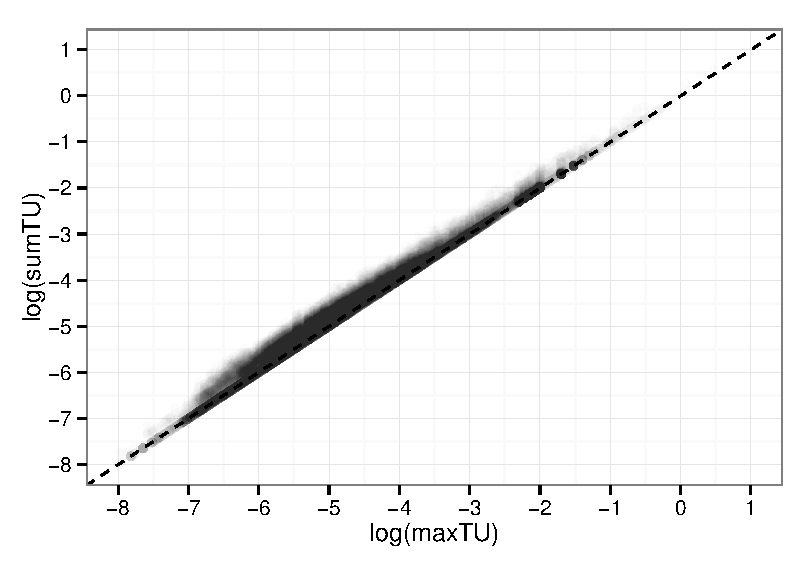
\includegraphics[width=\textwidth, keepaspectratio]{figs/tusum_tumax.pdf}
	    \column{.40\textwidth}
	        \begin{itemize}
	        	\item up to 50 compounds in one sample
	        	\item high correlation
	        	\item $\sim$ 0.5 TU increase 
	        	\item mainly one compound responsible for risk
	        \end{itemize}
	\end{columns}
\end{frame}

\begin{frame}
\frametitle{Simulations are worth their work, use them \emph{a priori}!}
Experimental design for dose-response experiments - a simulation
\begin{description}
	\item[webchem]{\url{http://edild.github.io/lc50_bias_sim/}}
\end{description}
	    	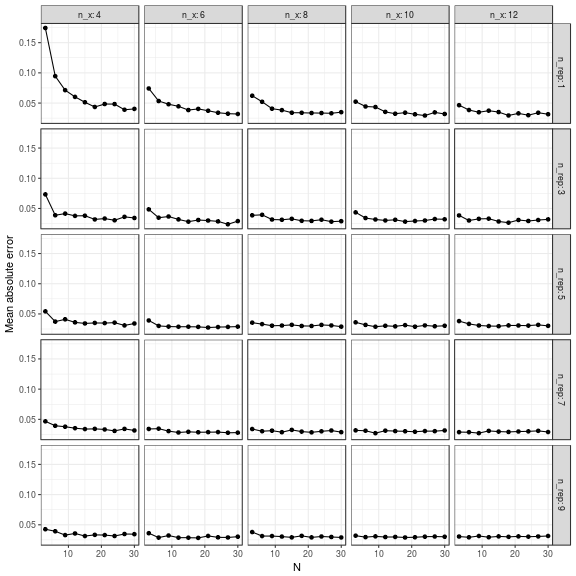
\includegraphics[width=0.6\textwidth, keepaspectratio]{figs/sim_drm.png}
\end{frame}



\begin{frame}
\frametitle{Reasons for observed RAC exceedances}
see notes on lecture on 16.12.2016

\end{frame}




\begin{frame}
\frametitle{Biotic field effects}
	\begin{columns}
	    \column{.49\textwidth}
	    	    	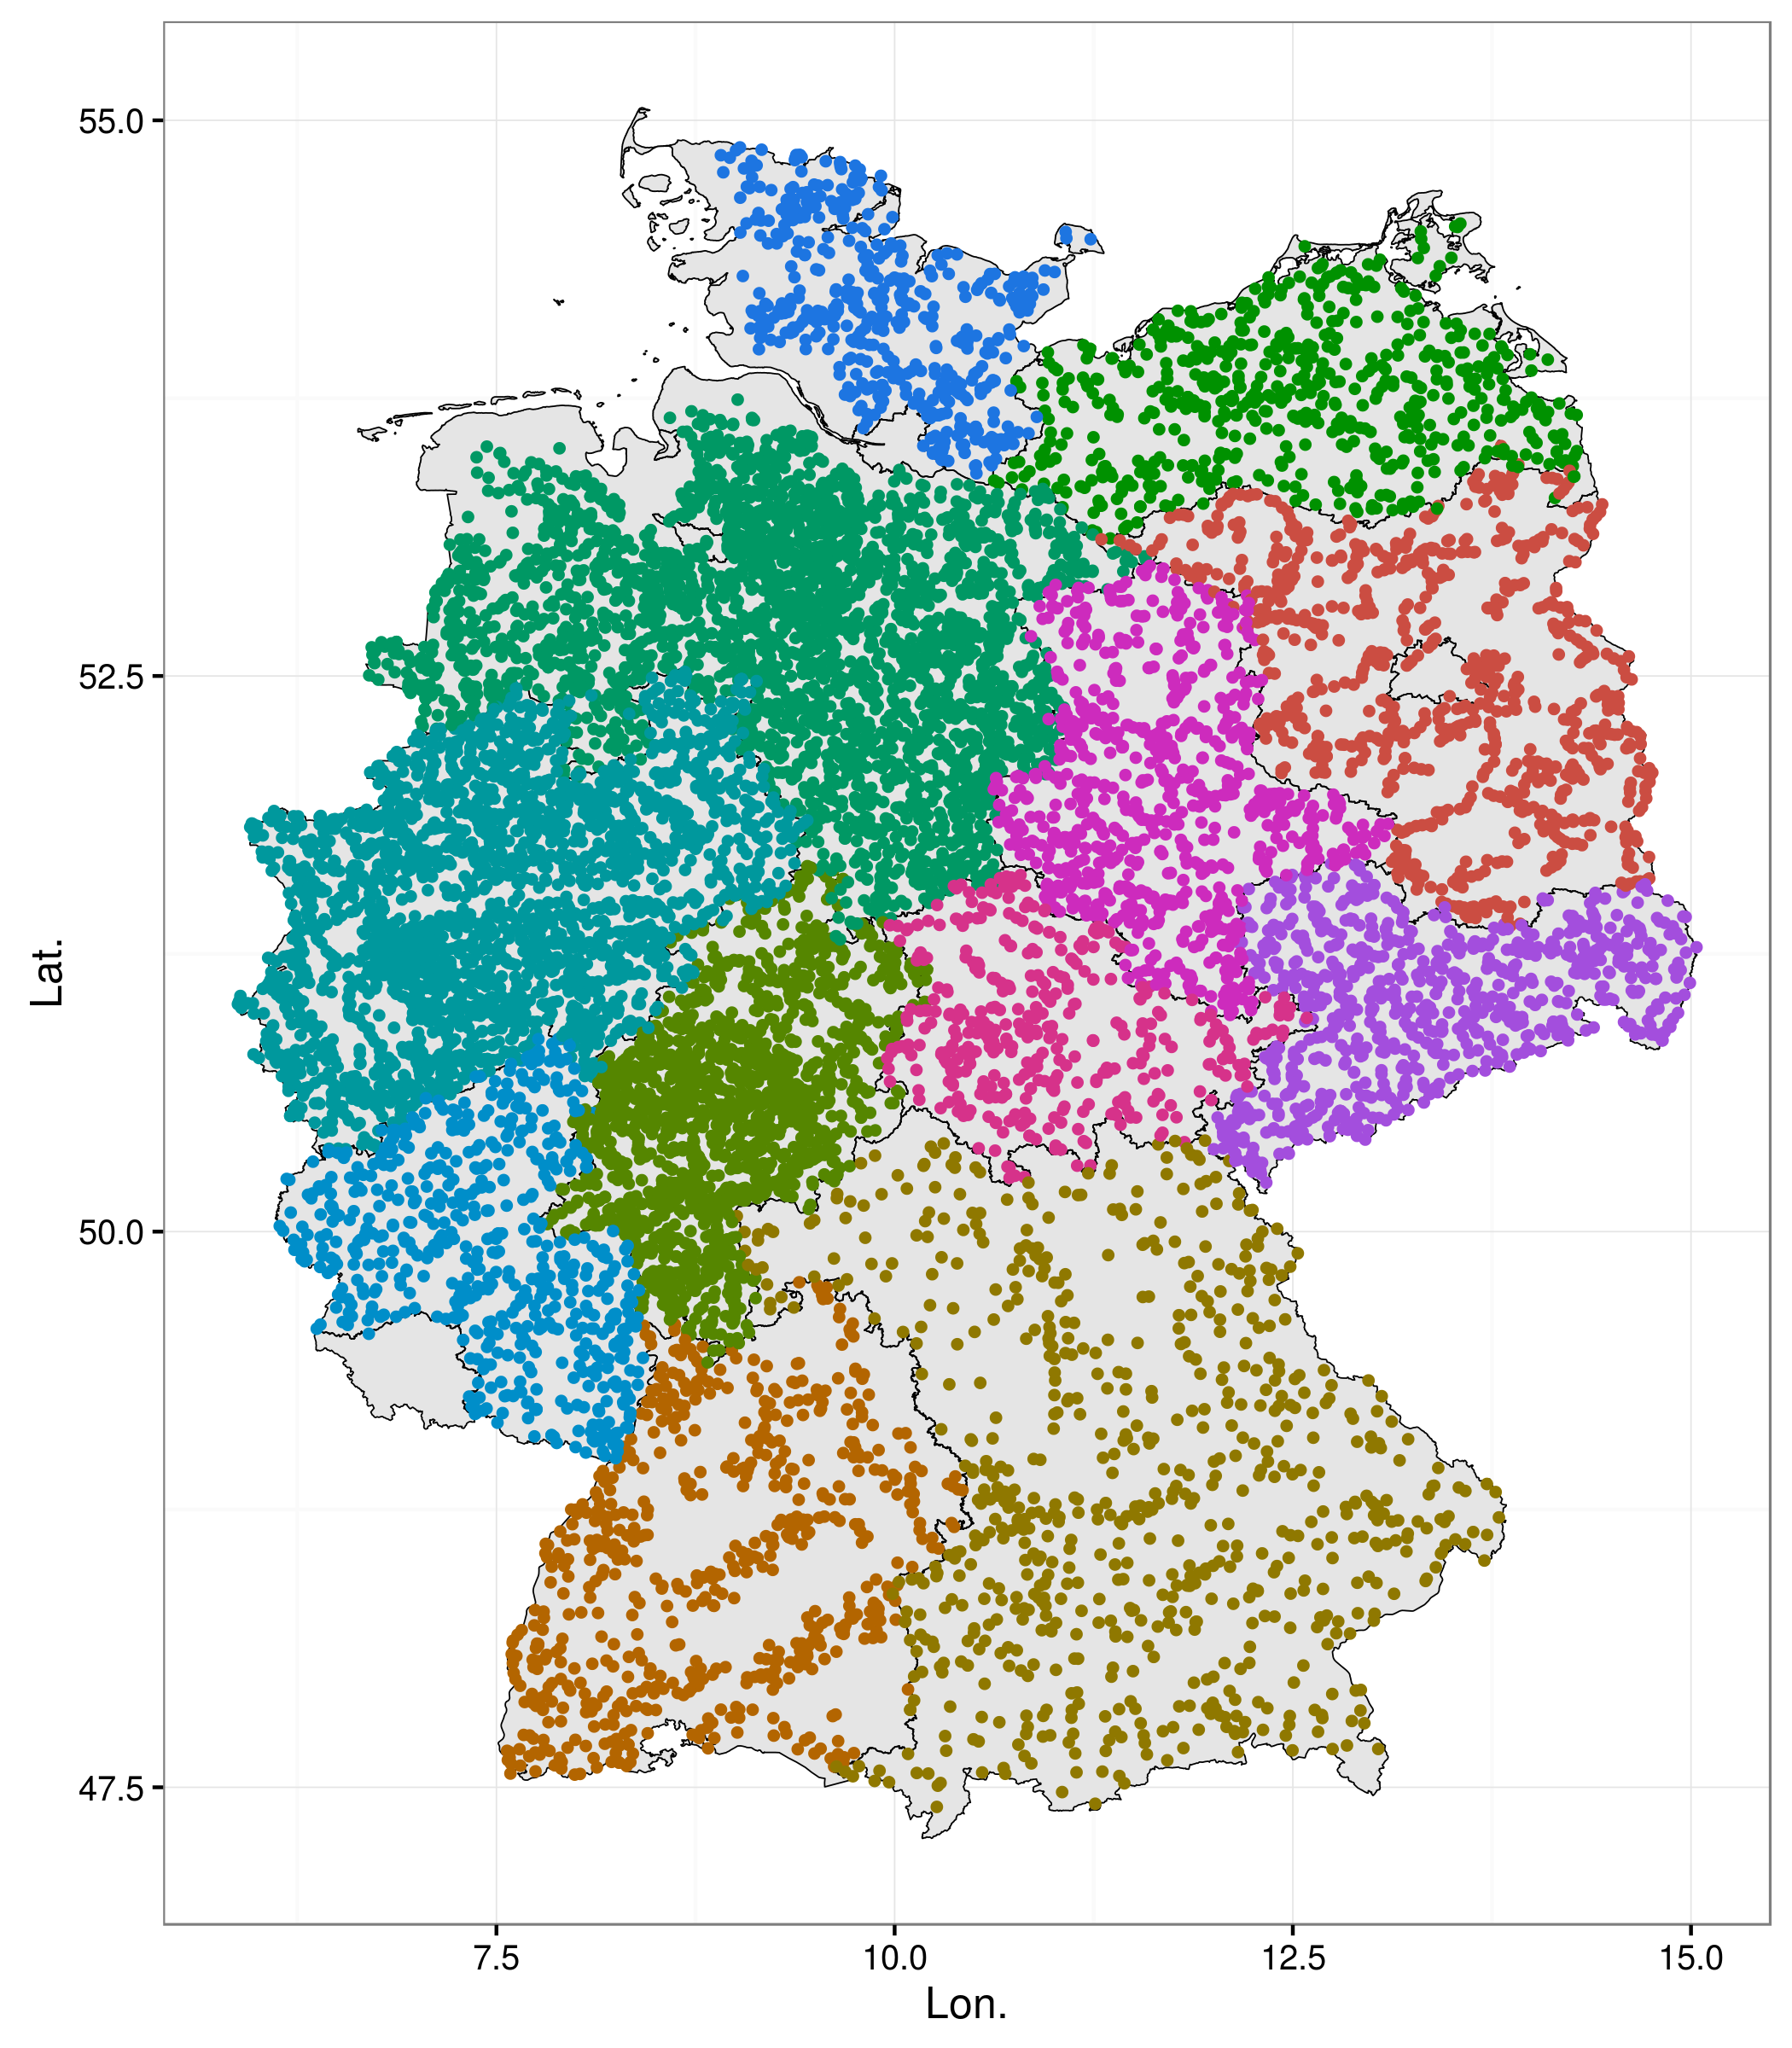
\includegraphics[width=\textwidth, keepaspectratio]{figs/mzb_map.png}
	    \column{.49\textwidth}
	        \begin{itemize}
	        	\item biological data with good spatial coverage
	        	\item 60\% of spatial congruence 
	        	\item Large scale effects largely unknown.
	        	\item Some work left...
	        	\item Future....
	        \end{itemize}
	\end{columns}

\end{frame}


\begin{frame}
\frametitle{Software}
\begin{description}
	\item[webchem]{\url{https://github.com/ropensci/webchem}}
	\item[taxize]{\url{https://github.com/ropensci/webchem}}
\end{description}

Stable versions also on CRAN...

\end{frame}



% ------------------------------
\end{document}
